\clearpage
%%%%%%%%%%%%%%%%%%%%%%%% N-1 plots %%%%%%%%%%%%%%%%%%%%%%%
%\section{N-1 plots}

\begin{figure}[h]
  \centering
%    \subfigure[]{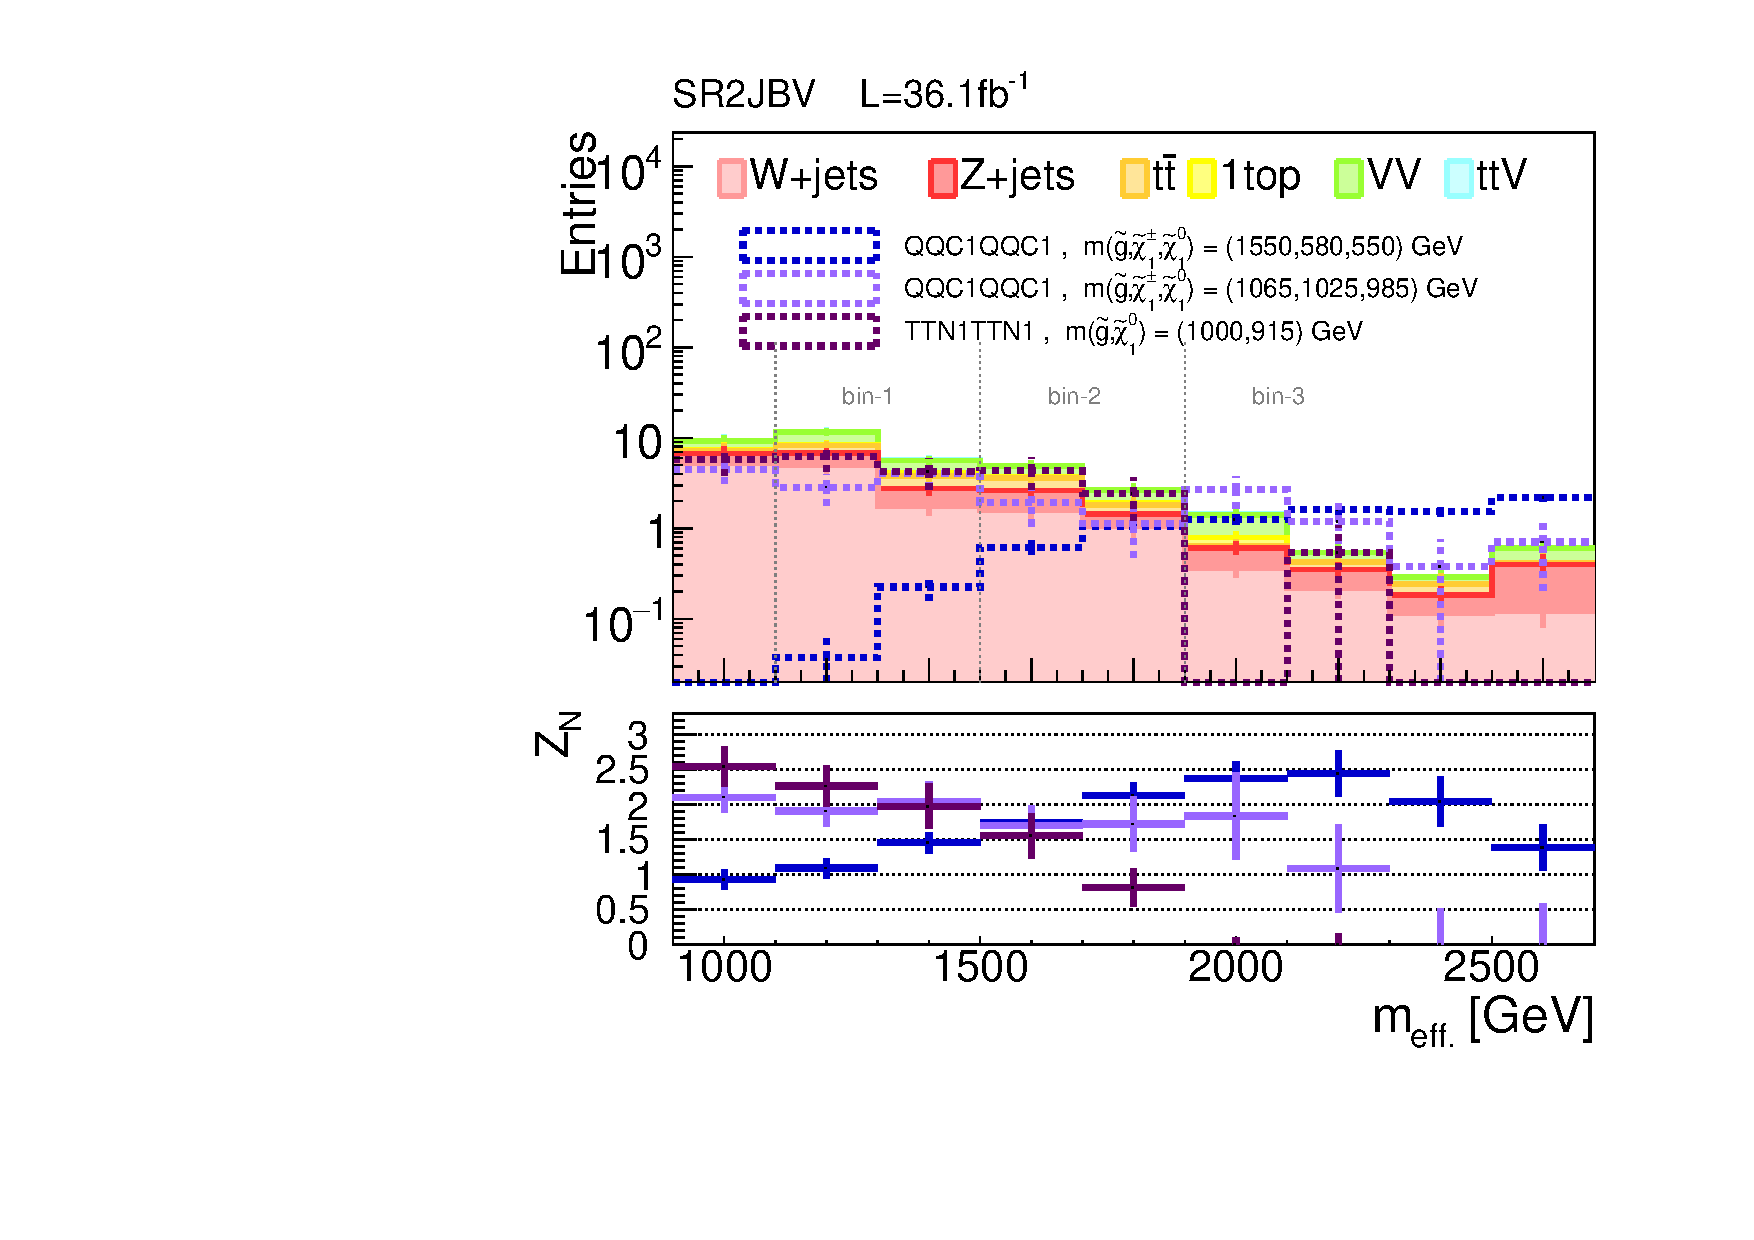
\includegraphics[width=0.45\textwidth]{figures/SRdefinition/N1plot/meffInc30_2JMEFFInclBV.pdf}}
    \subfigure[]{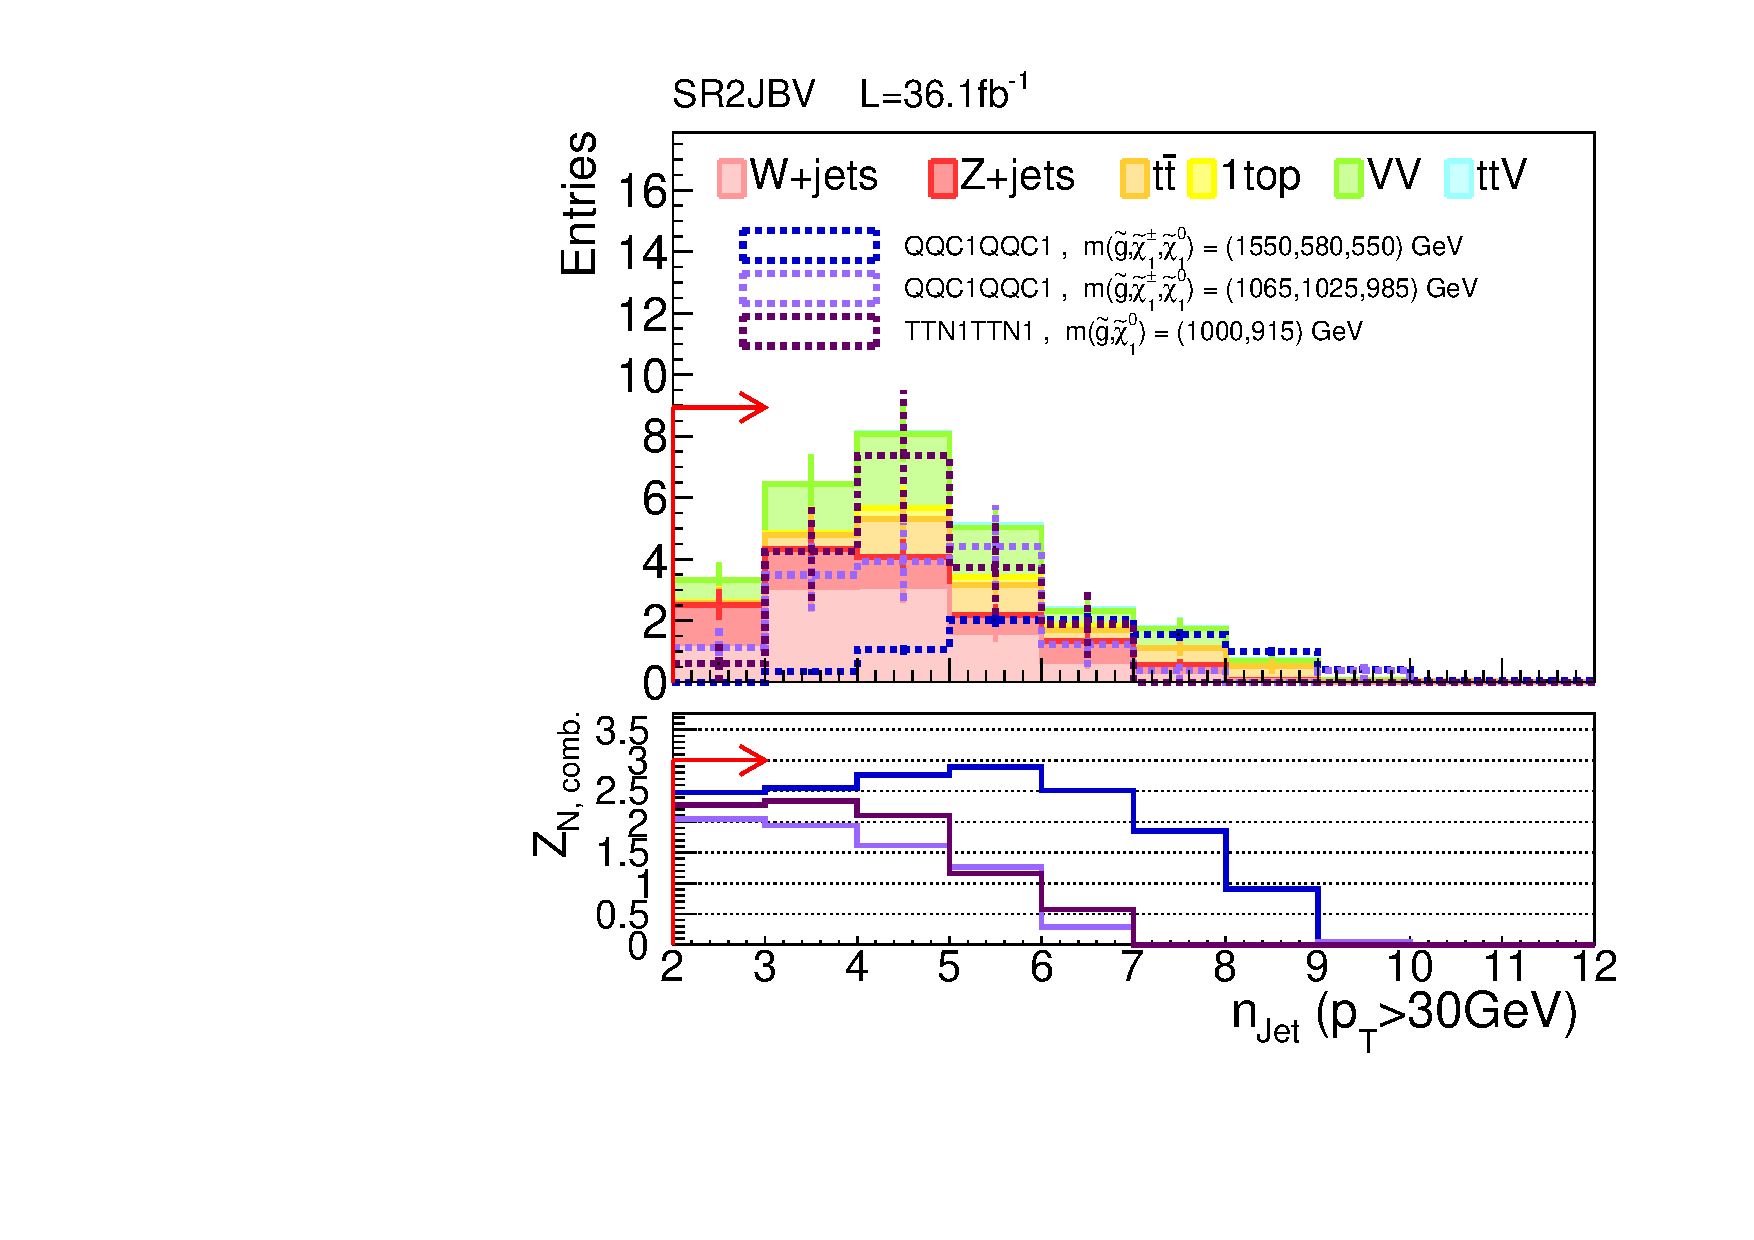
\includegraphics[width=0.45\textwidth]{figures/SRdefinition/N1plot/nJet30_2JMEFFInclBV.pdf}}
%    \subfigure[]{\includegraphics[width=0.45\textwidth]{figures/SRdefinition/N1plot/lep1Pt_2JMEFFInclBV.pdf}}
    \subfigure[]{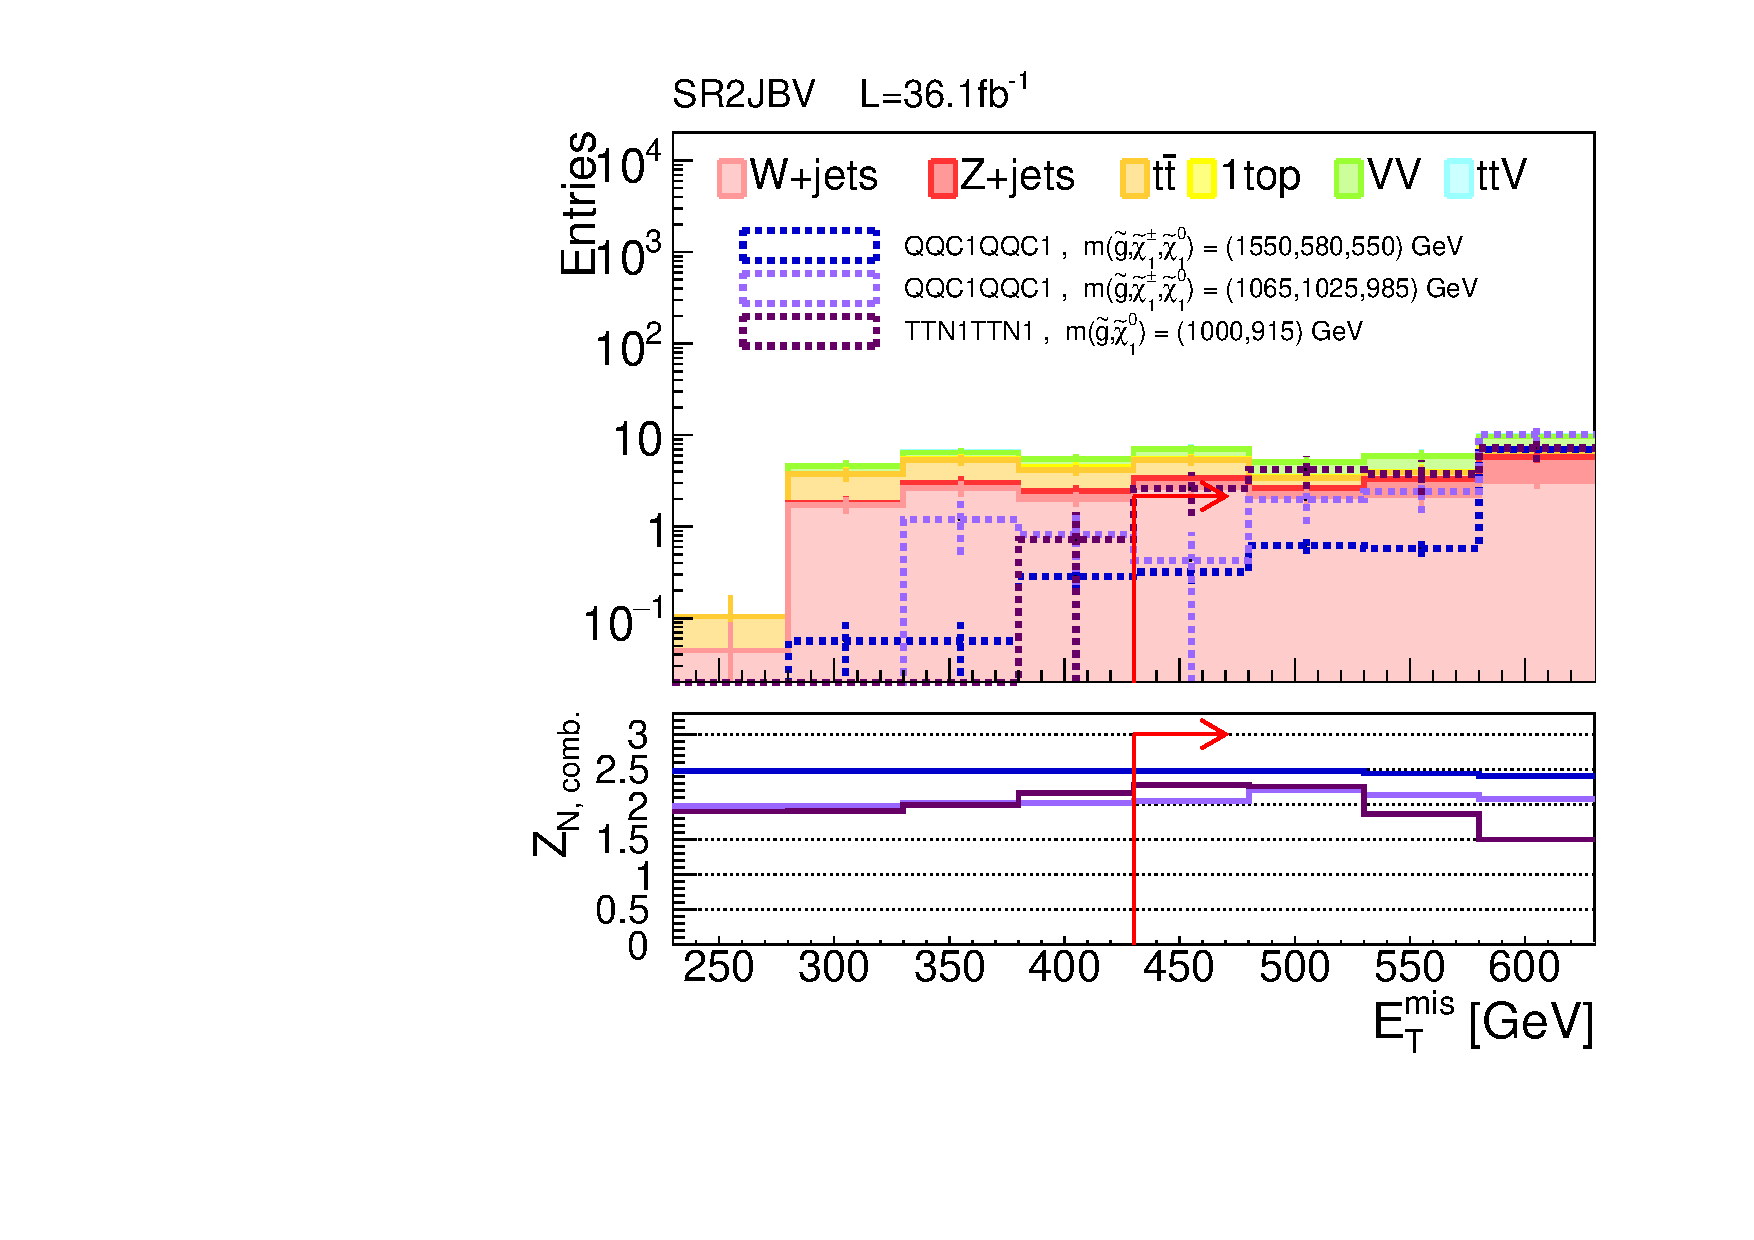
\includegraphics[width=0.45\textwidth]{figures/SRdefinition/N1plot/met_2JMEFFInclBV.pdf}}
    \subfigure[]{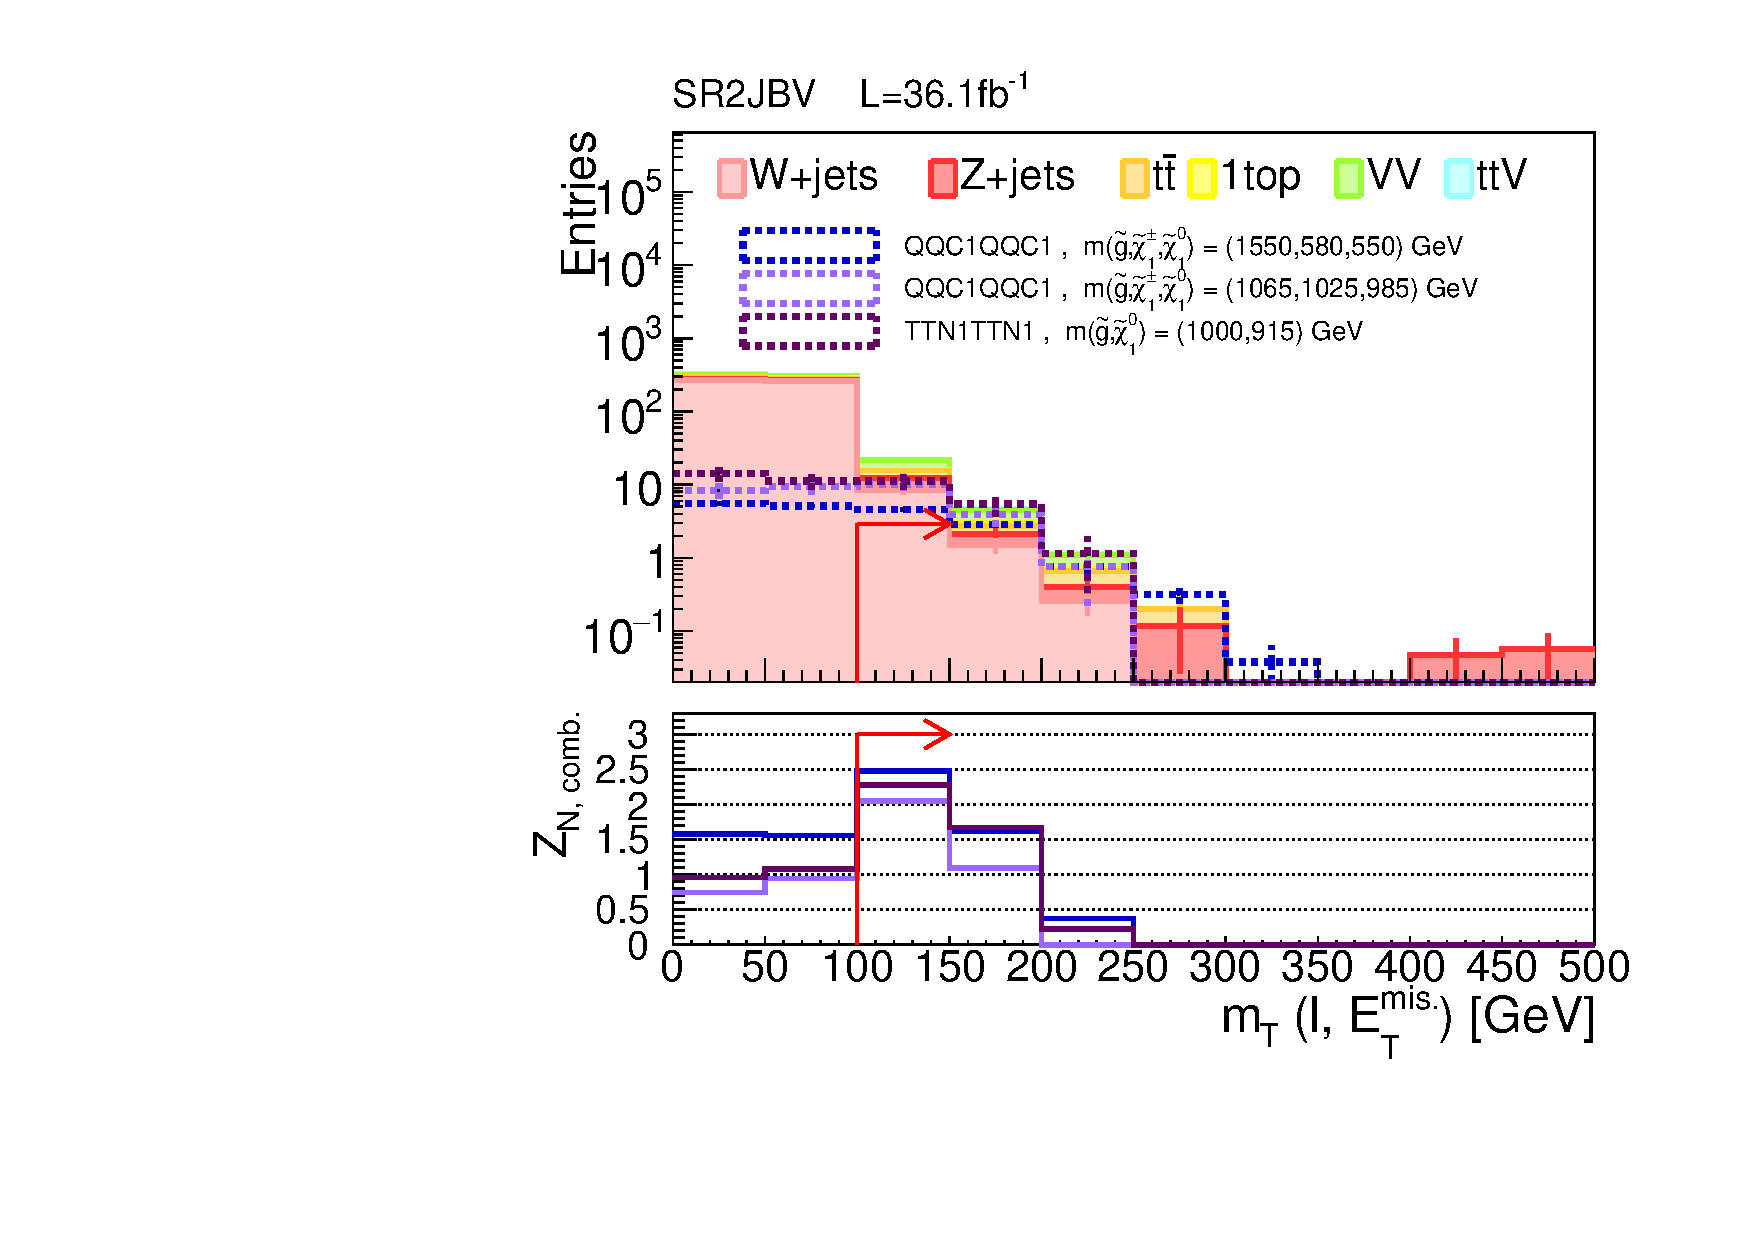
\includegraphics[width=0.45\textwidth]{figures/SRdefinition/N1plot/mt_2JMEFFInclBV.pdf}}
    \subfigure[]{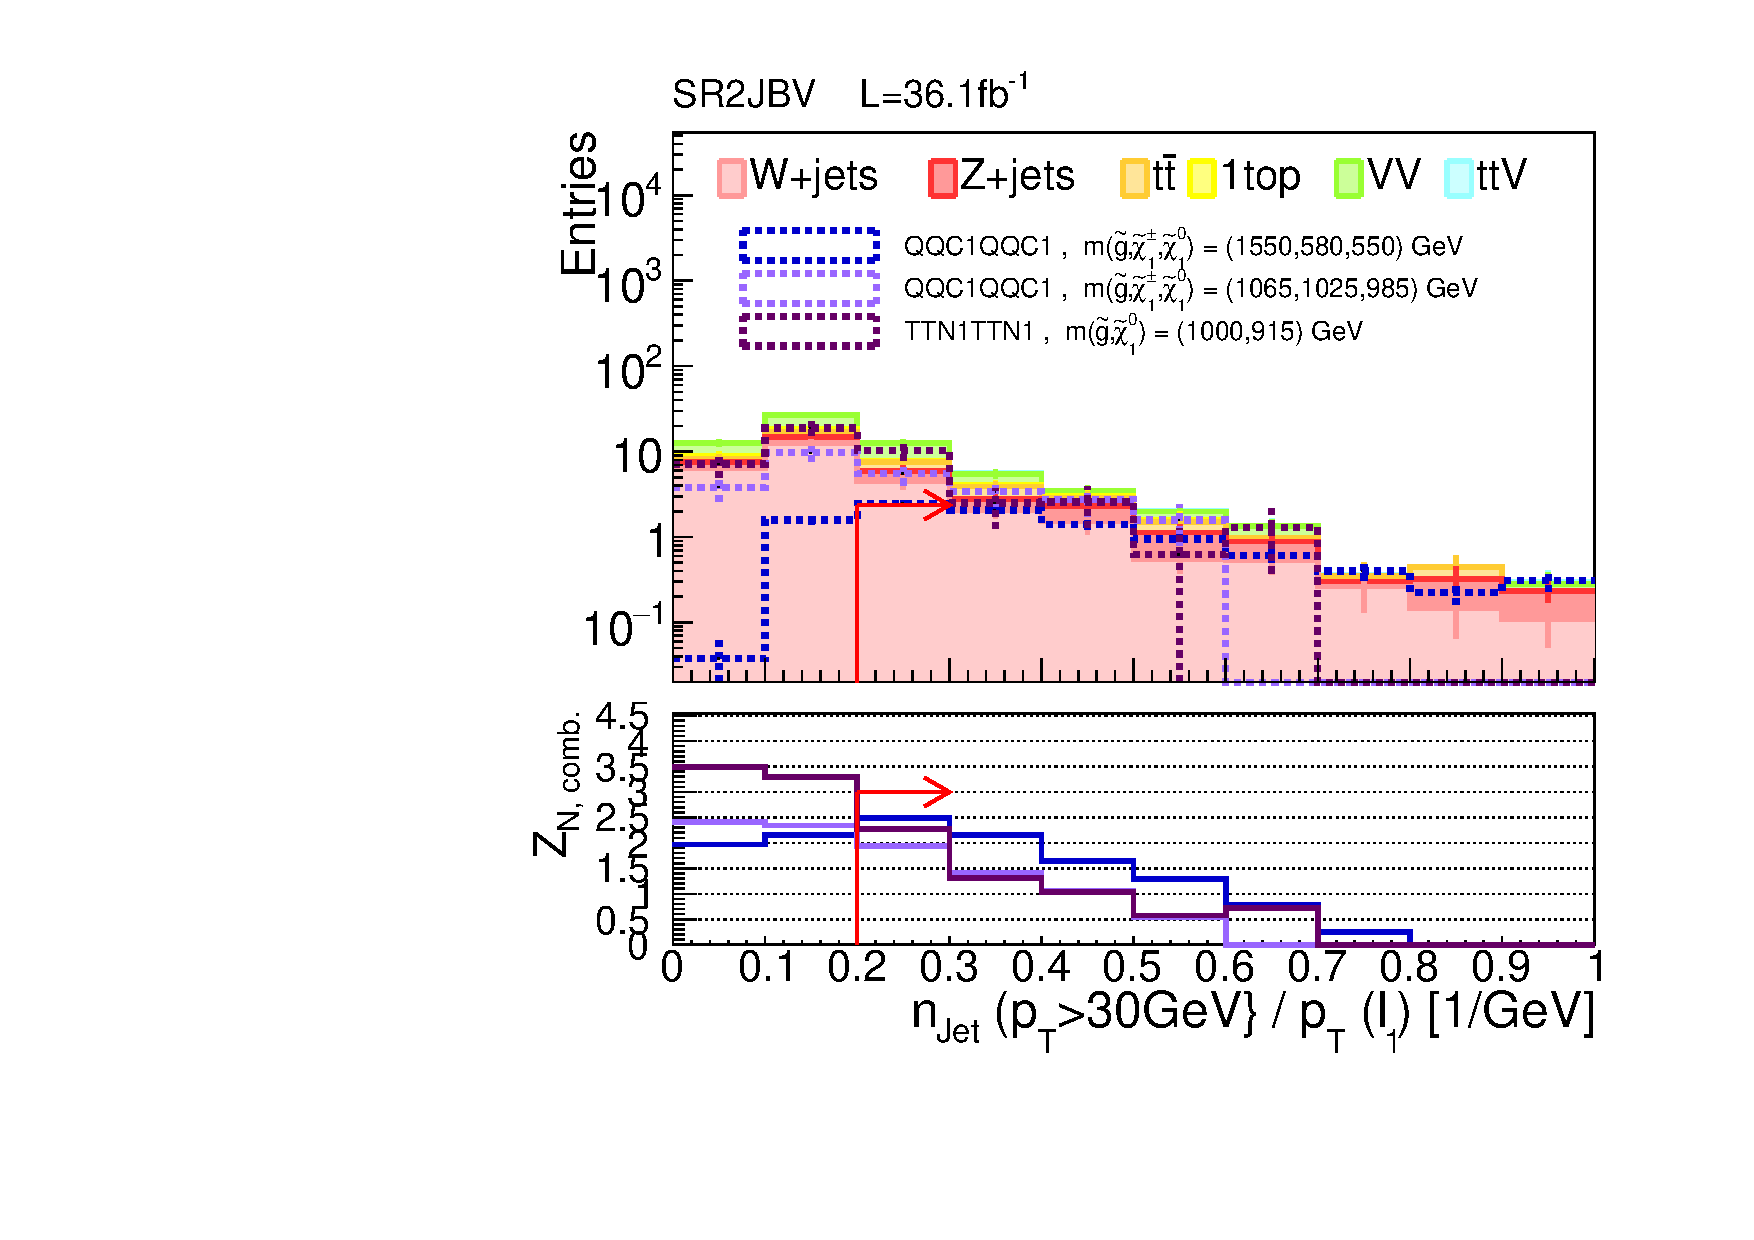
\includegraphics[width=0.45\textwidth]{figures/SRdefinition/N1plot/nJetOverLep1Pt_2JMEFFInclBV.pdf}}
    \subfigure[]{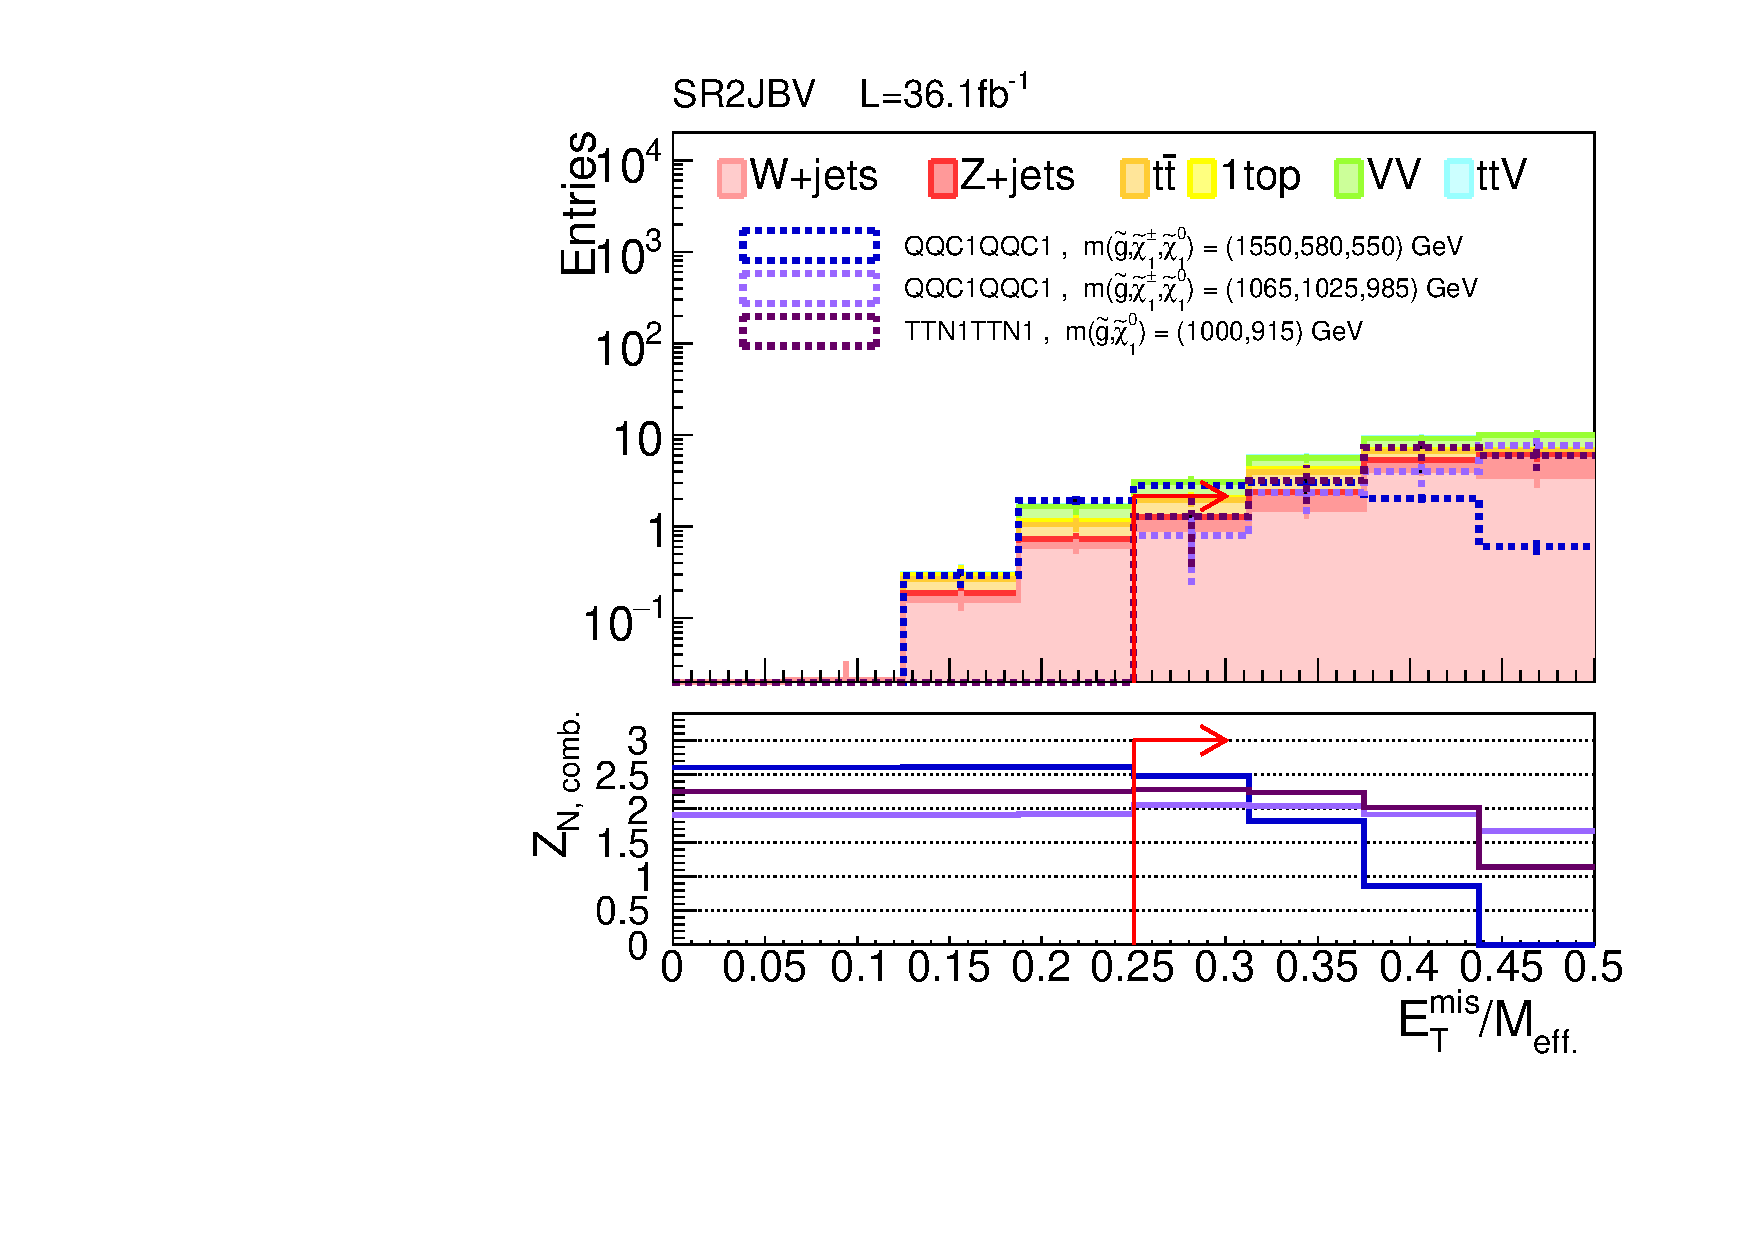
\includegraphics[width=0.45\textwidth]{figures/SRdefinition/N1plot/metOverMeff_2JMEFFInclBV.pdf}}
    \subfigure[]{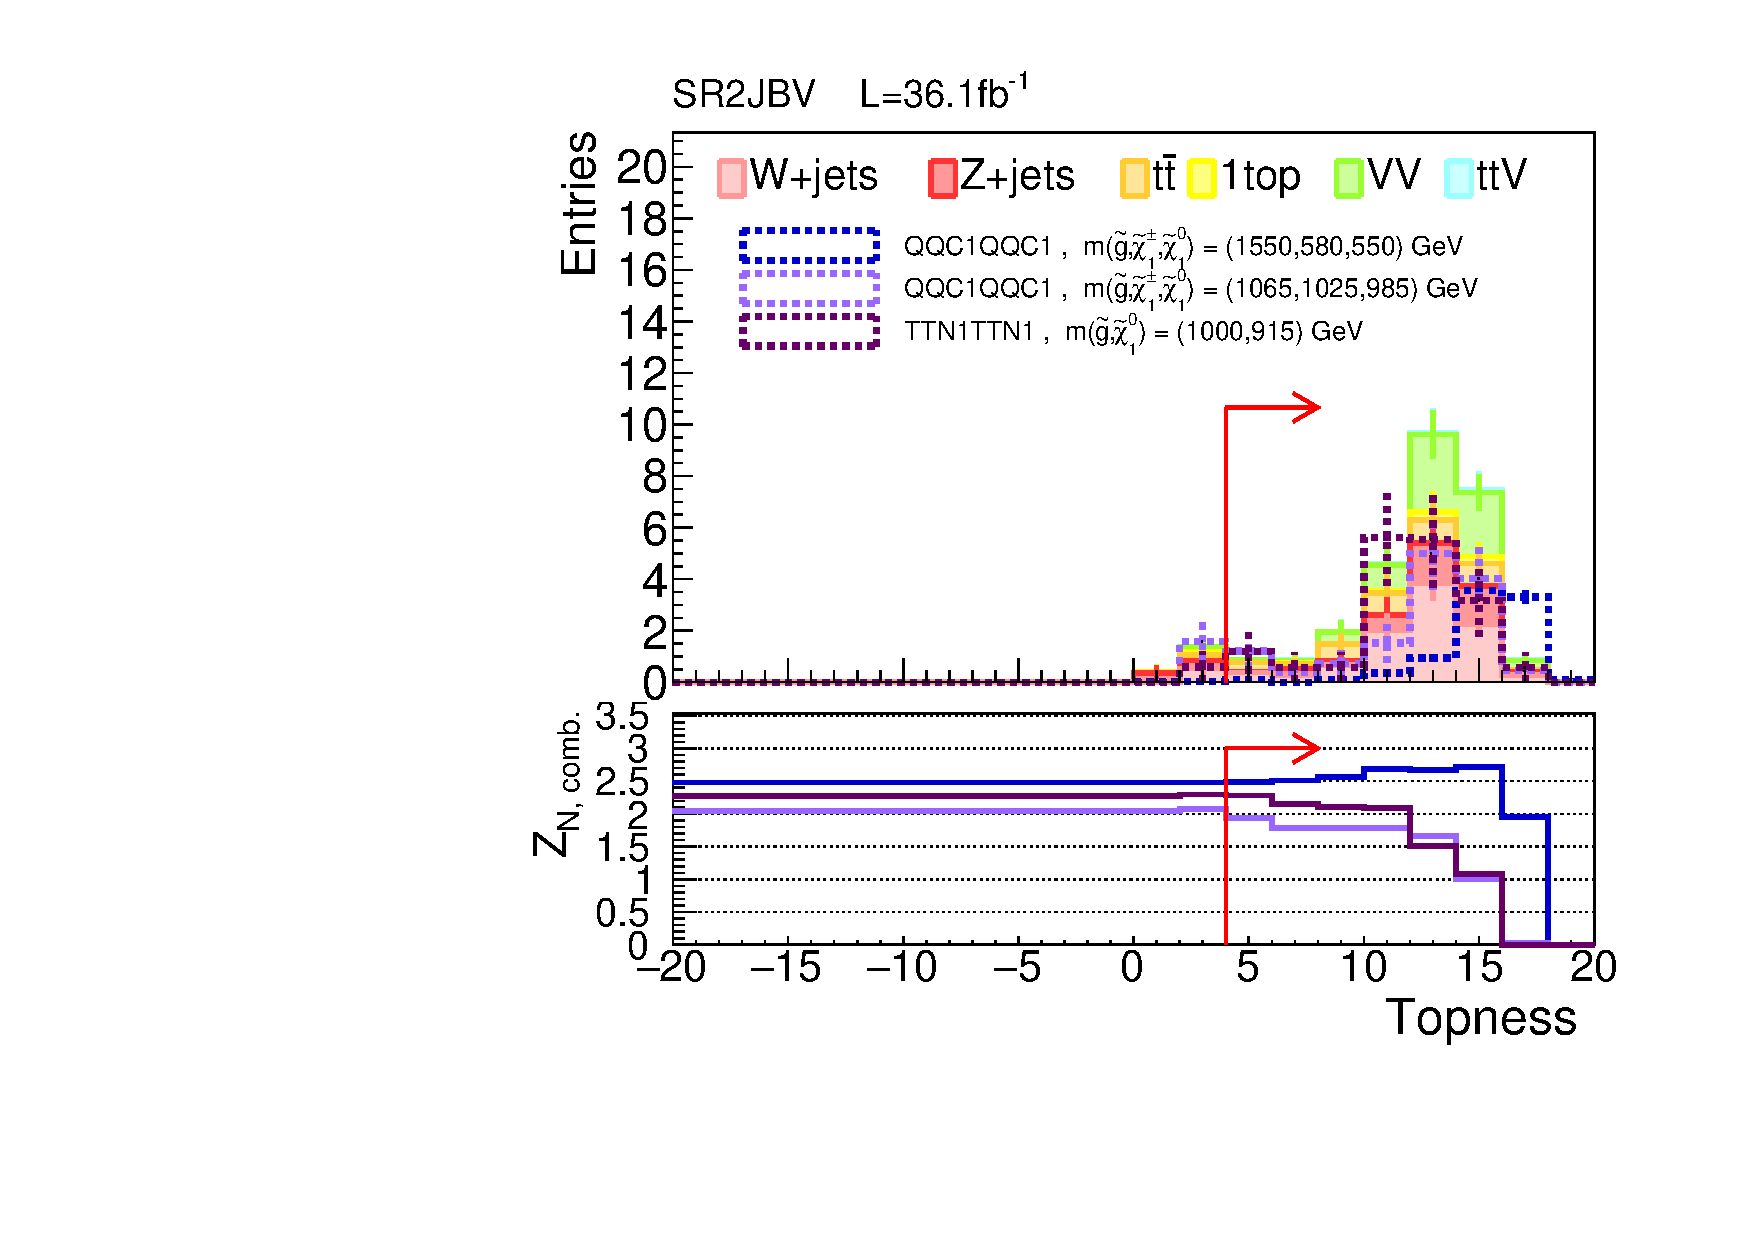
\includegraphics[width=0.45\textwidth]{figures/SRdefinition/N1plot/topNess_2JMEFFInclBV.pdf}}
    \caption{ 
    N-1 plots for the b-vetoed (BV) slices of the optimized \textbf{2J} signal regions.
    Bottom row presents the combined significace over the $\meffInc$ bins defined in Eq. \ref{ZNcomb}.
    \label{fig::SRdefinition::N1plots_2JMEFFInclBV}
    }
\end{figure}
 

\clearpage
\begin{figure}[h]
  \centering
%    \subfigure[]{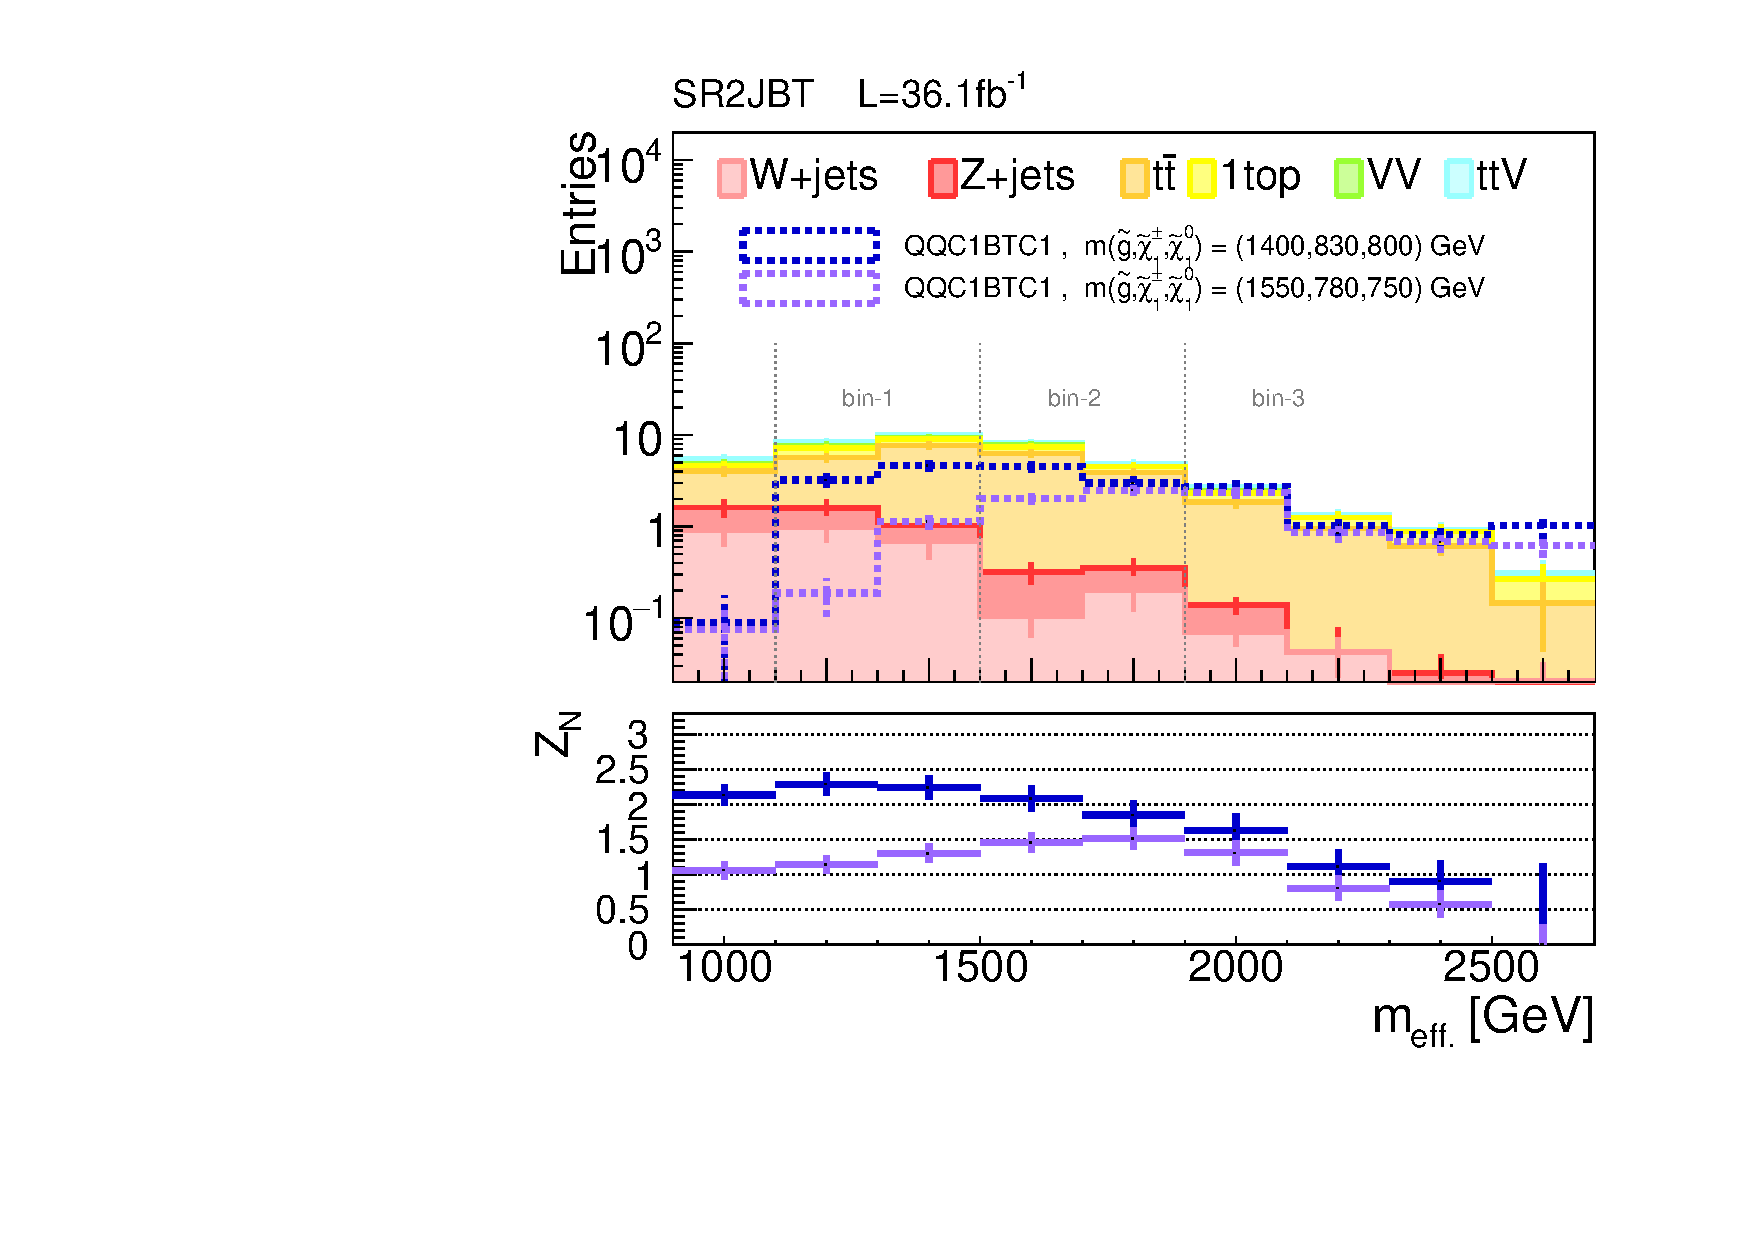
\includegraphics[width=0.45\textwidth]{figures/SRdefinition/N1plot/meffInc30_2JMEFFInclBT.pdf}}
    \subfigure[]{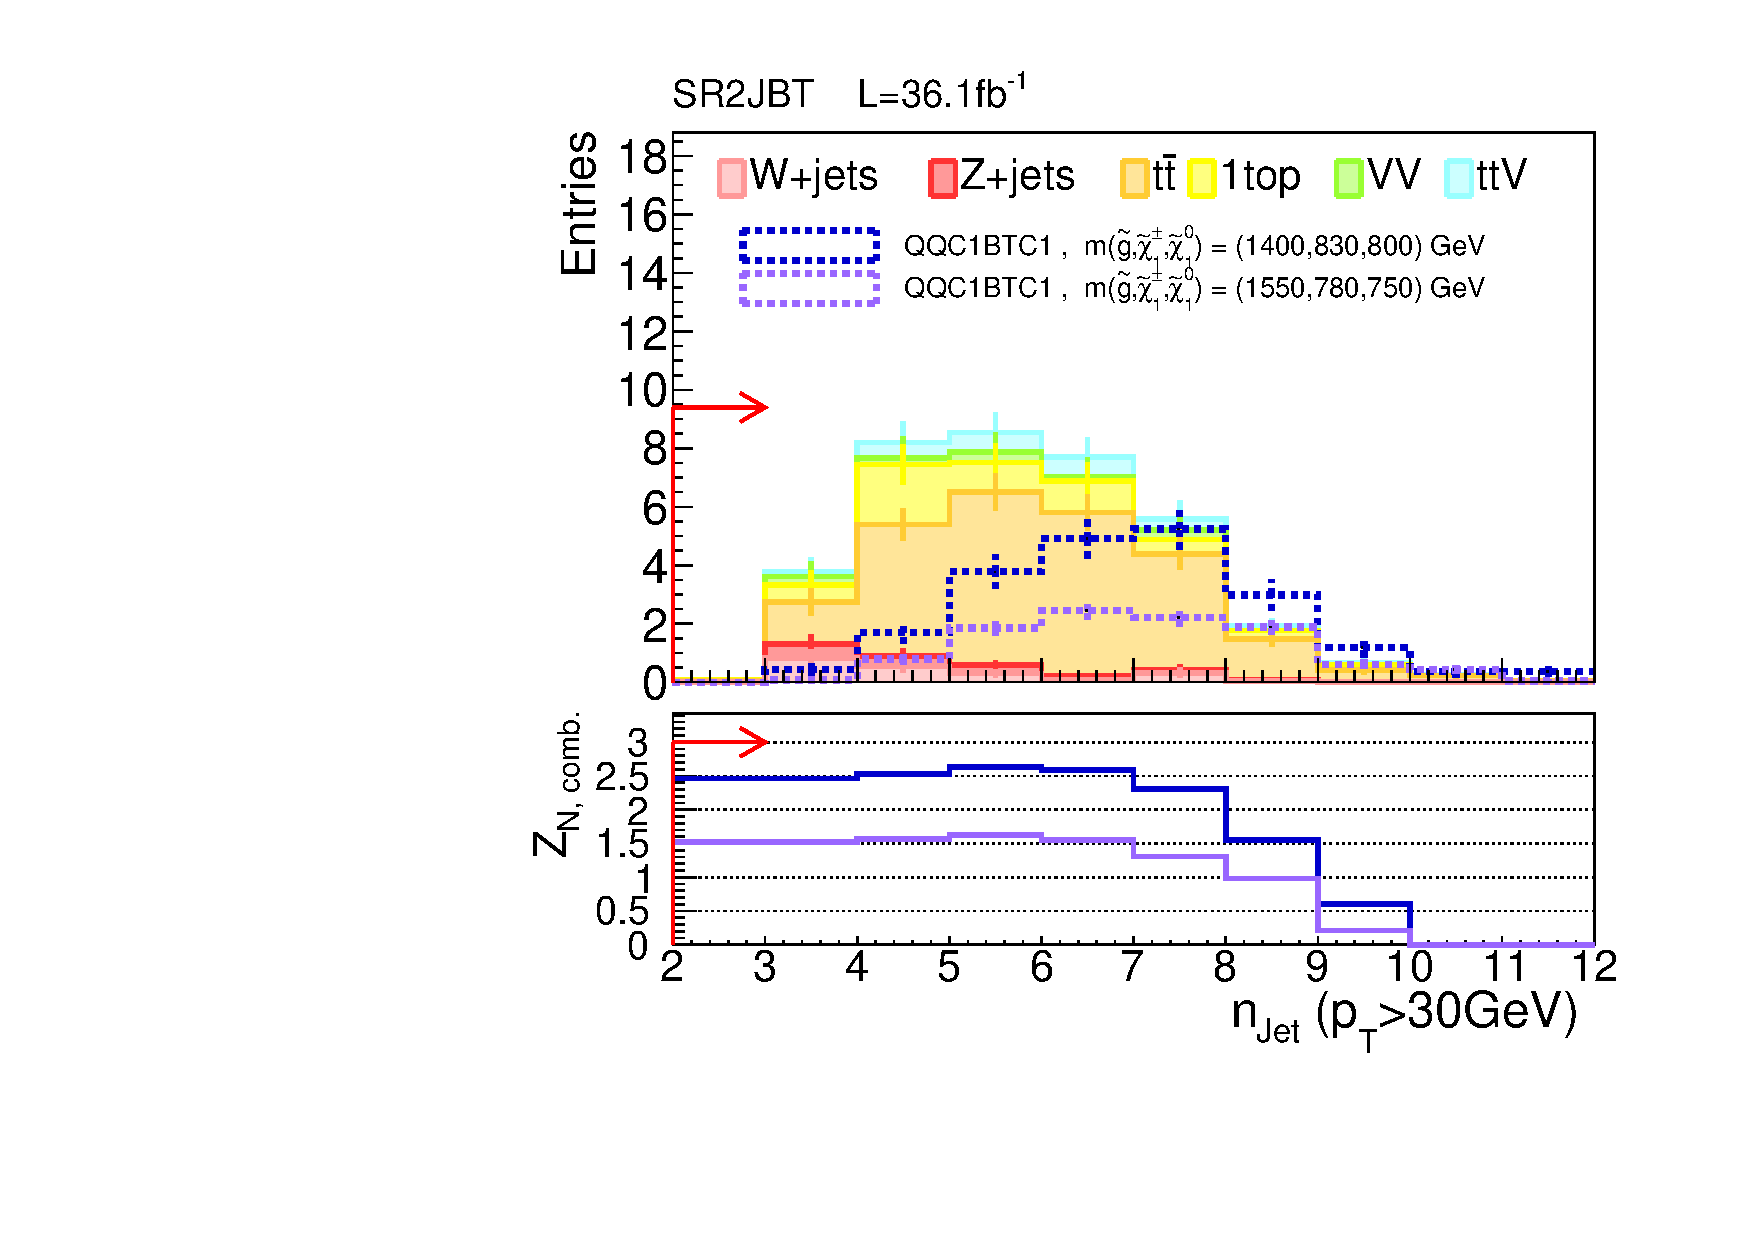
\includegraphics[width=0.45\textwidth]{figures/SRdefinition/N1plot/nJet30_2JMEFFInclBT.pdf}}
%    \subfigure[]{\includegraphics[width=0.45\textwidth]{figures/SRdefinition/N1plot/lep1Pt_2JMEFFInclBT.pdf}}
    \subfigure[]{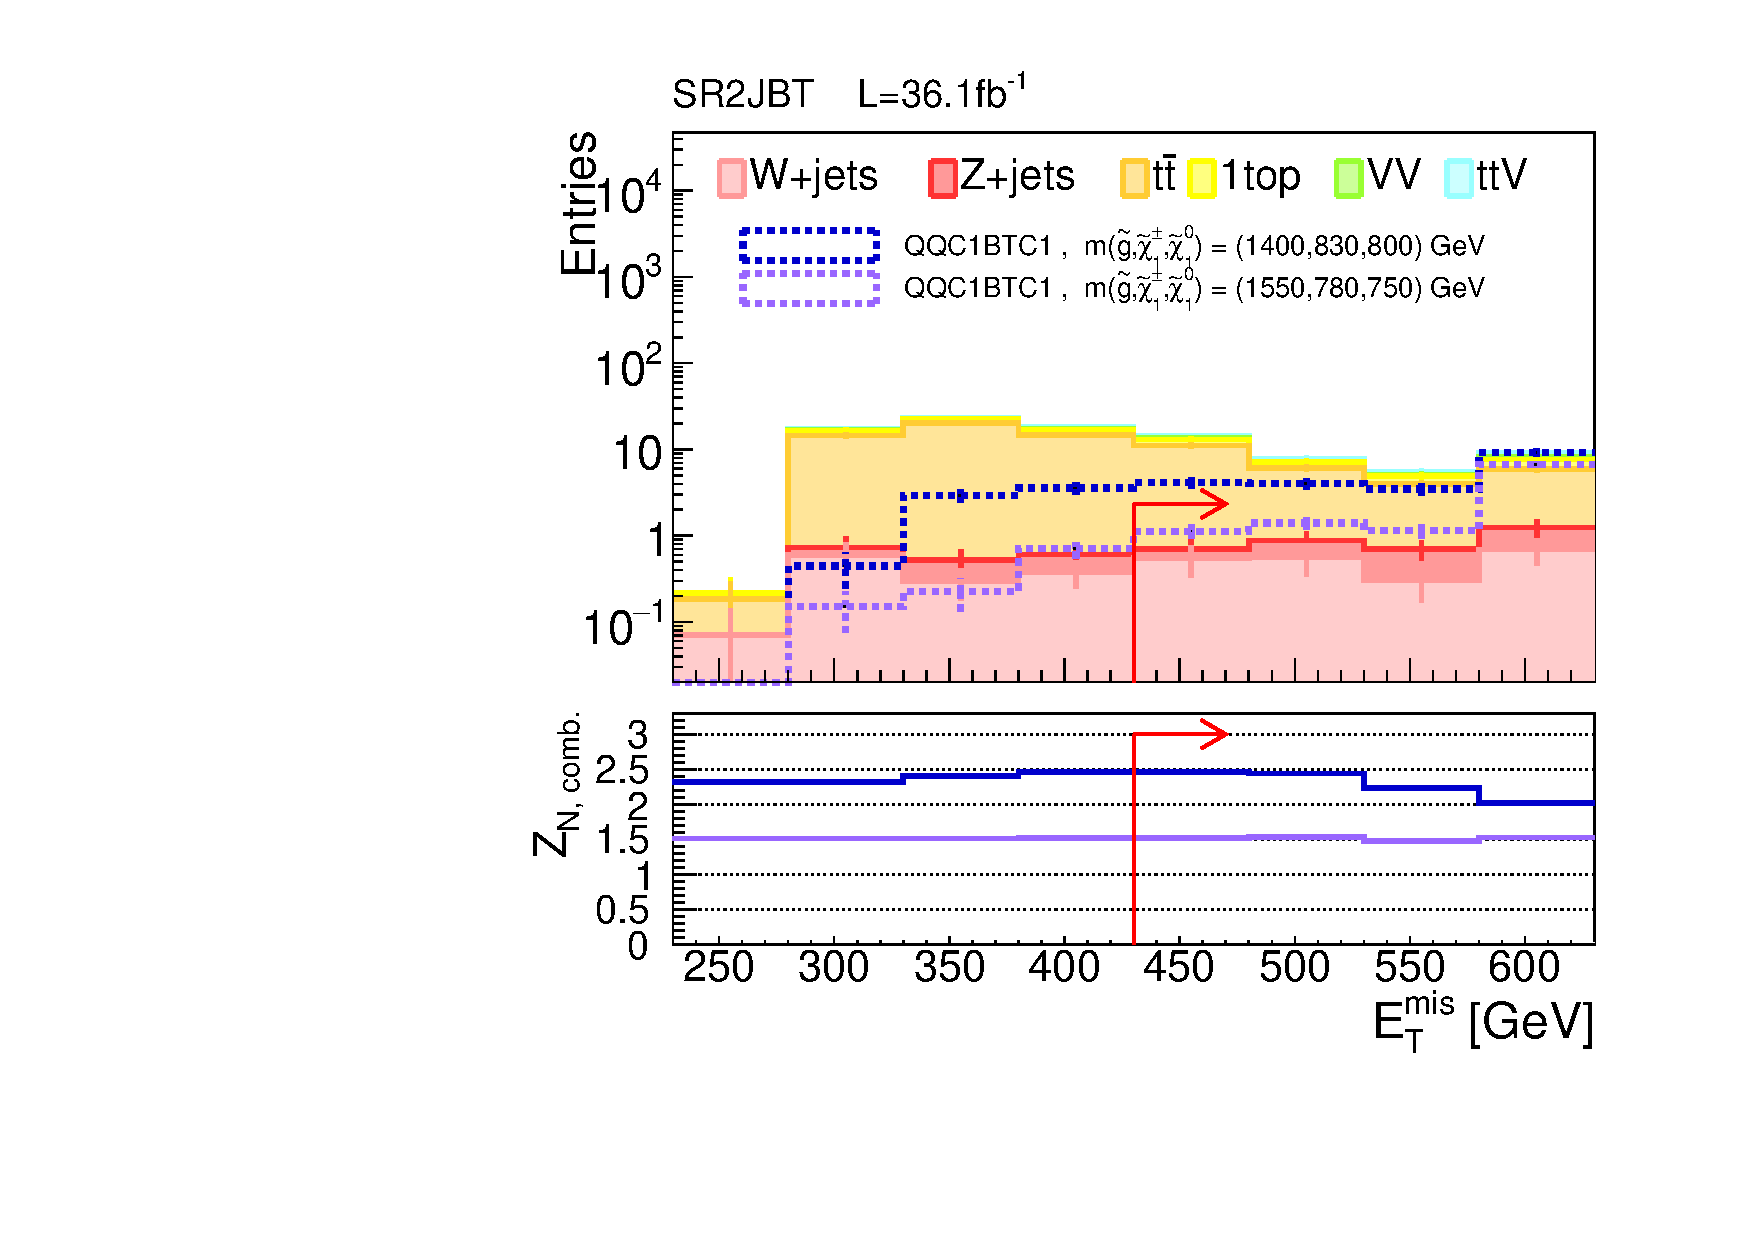
\includegraphics[width=0.45\textwidth]{figures/SRdefinition/N1plot/met_2JMEFFInclBT.pdf}}
    \subfigure[]{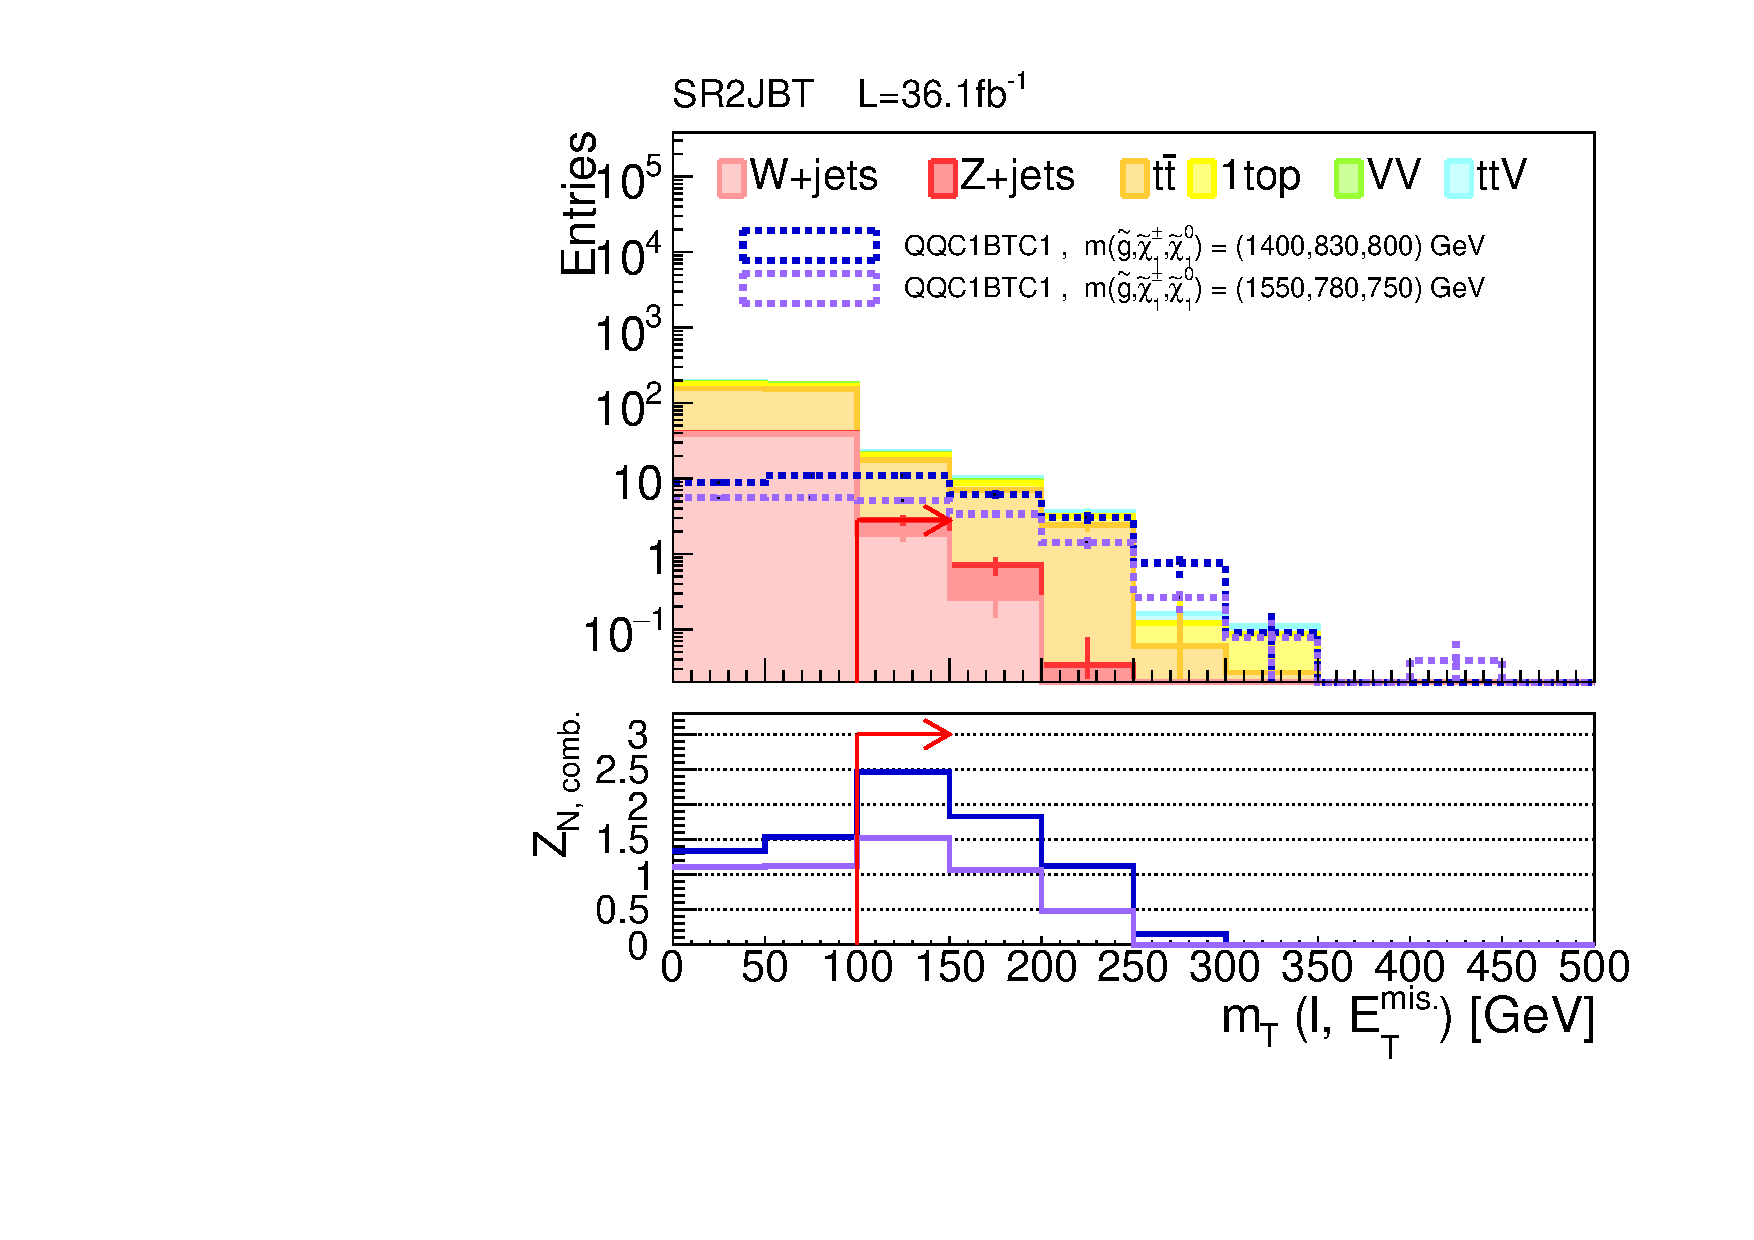
\includegraphics[width=0.45\textwidth]{figures/SRdefinition/N1plot/mt_2JMEFFInclBT.pdf}}
    \subfigure[]{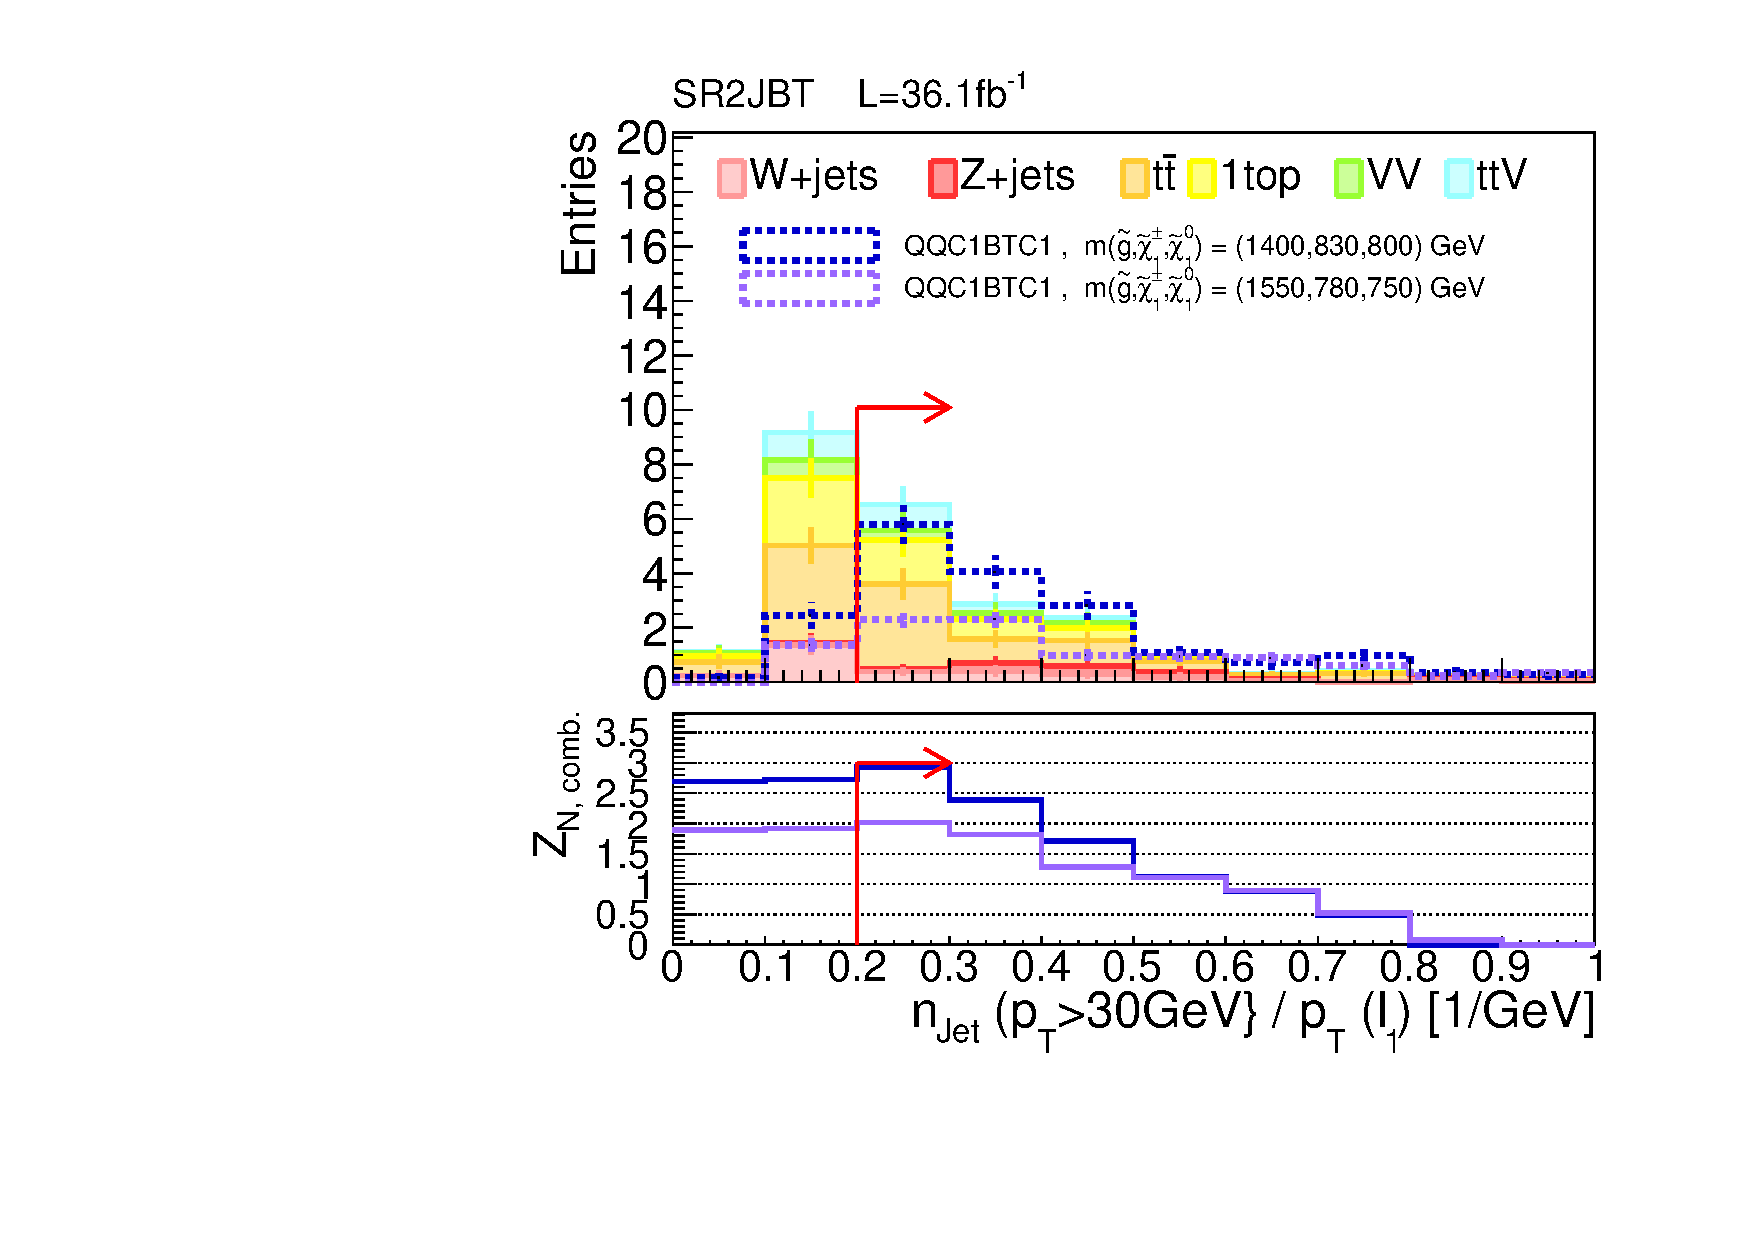
\includegraphics[width=0.45\textwidth]{figures/SRdefinition/N1plot/nJetOverLep1Pt_2JMEFFInclBT.pdf}}
    \subfigure[]{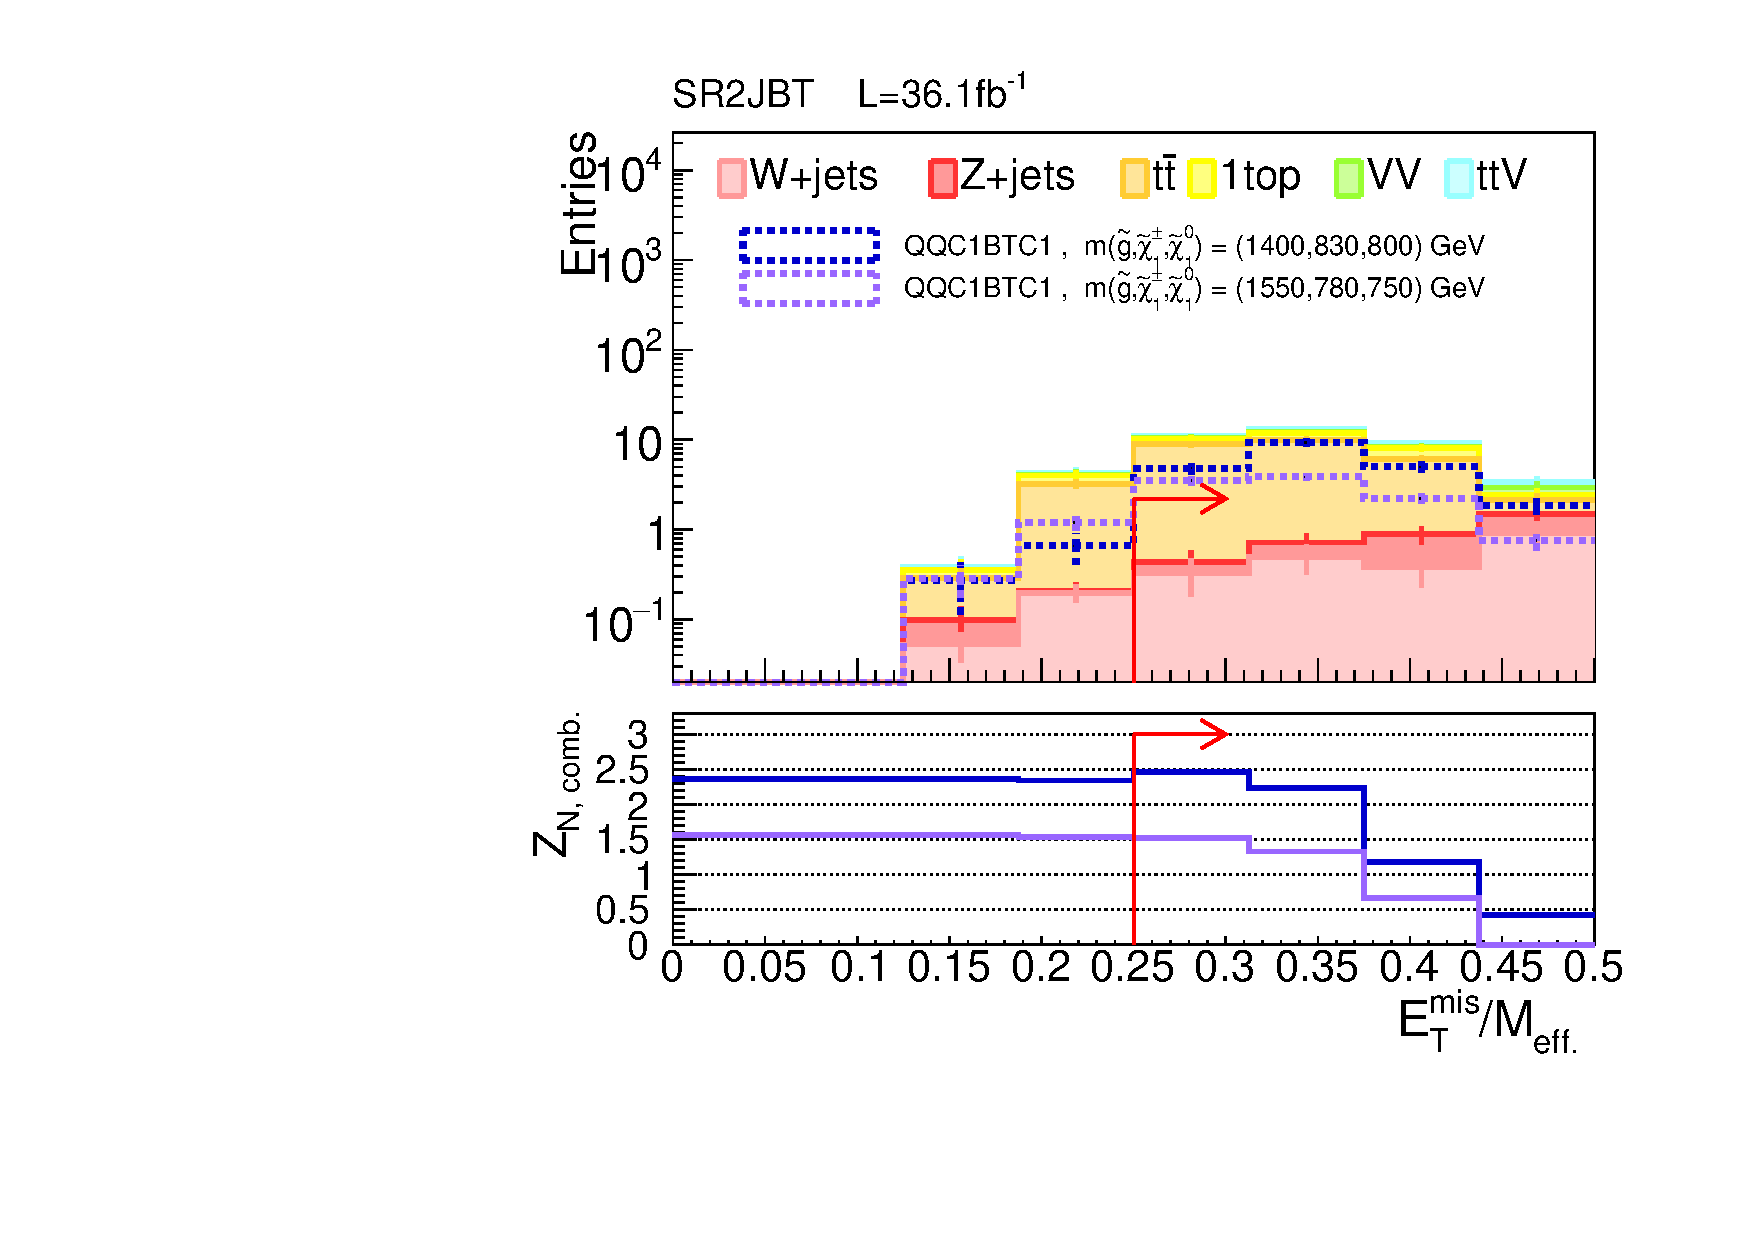
\includegraphics[width=0.45\textwidth]{figures/SRdefinition/N1plot/metOverMeff_2JMEFFInclBT.pdf}}
    \subfigure[]{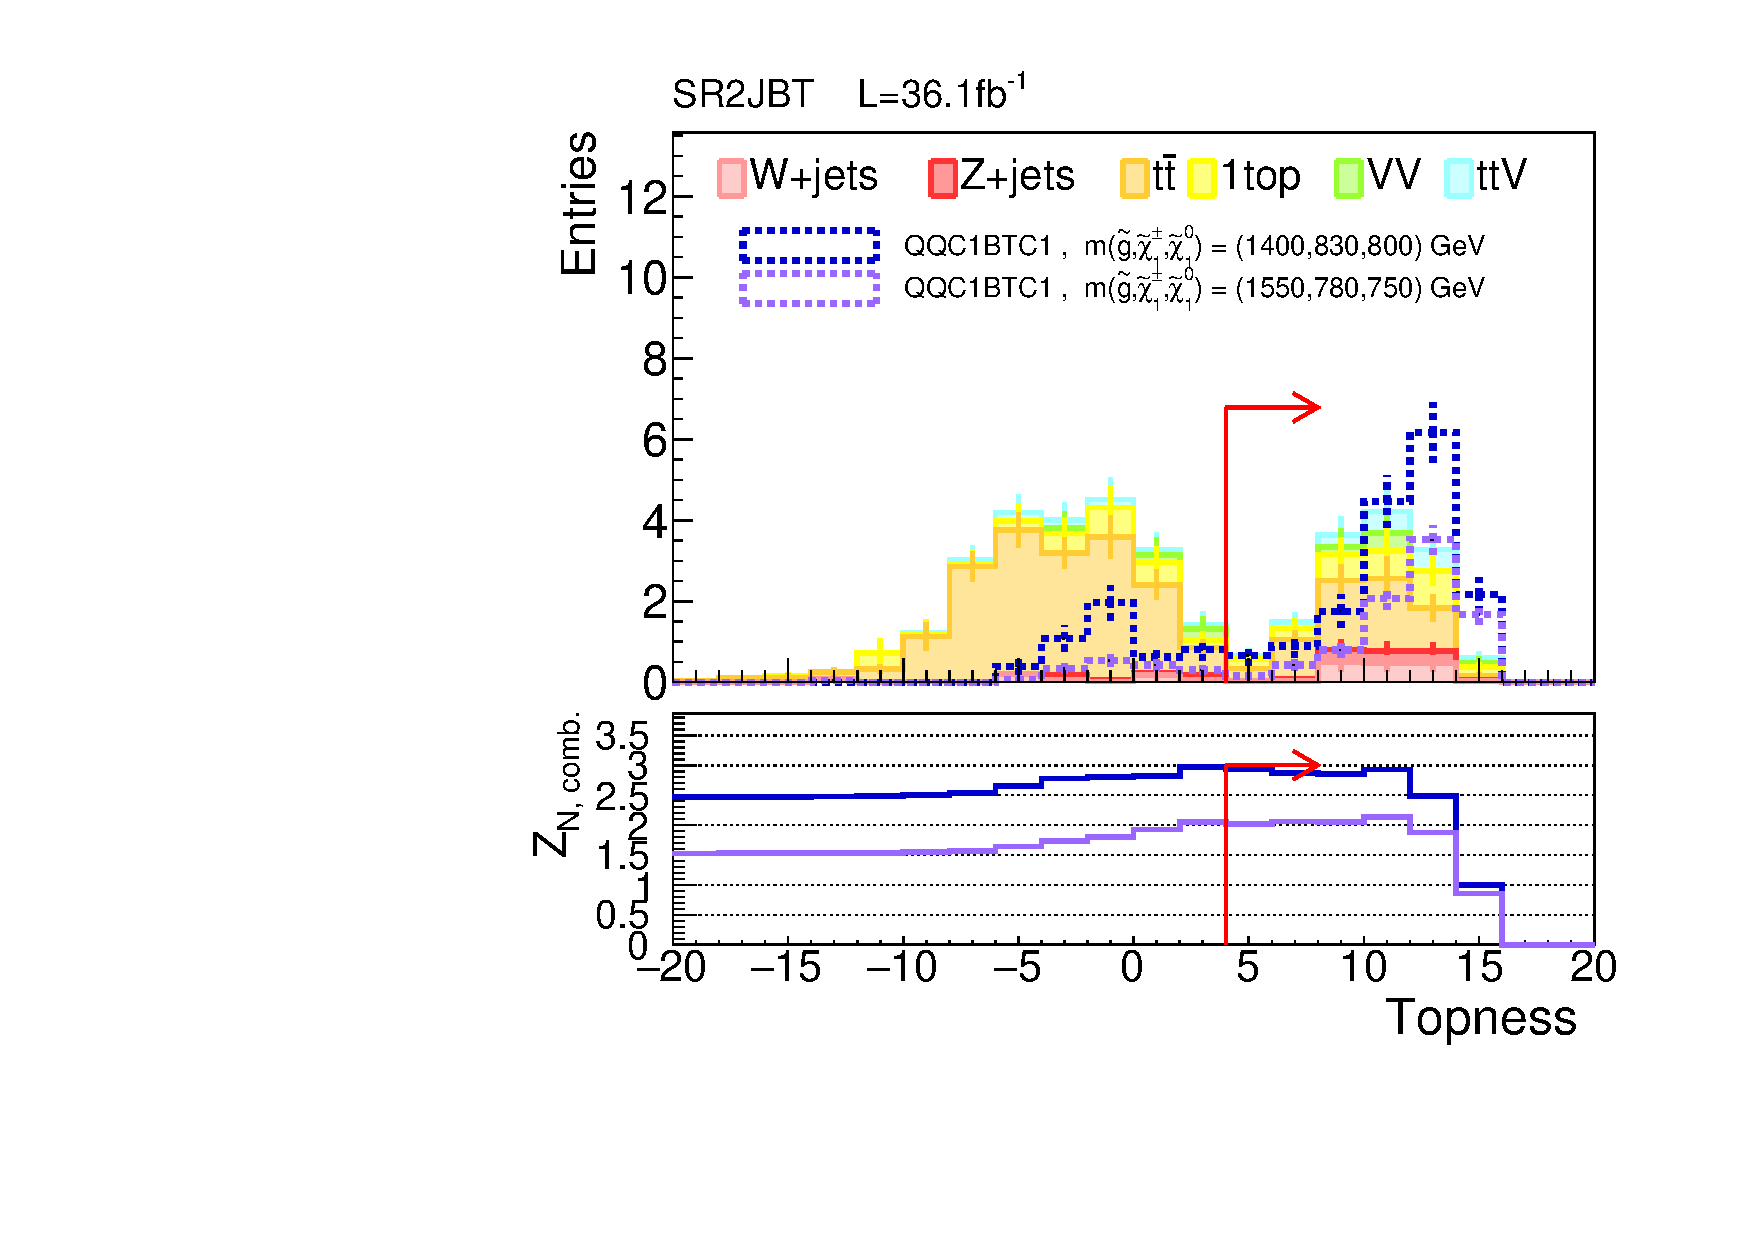
\includegraphics[width=0.45\textwidth]{figures/SRdefinition/N1plot/topNess_2JMEFFInclBT.pdf}}
    \caption{ 
    N-1 plots for the b-tagged (BT) slices of the optimized \textbf{2J} signal regions.
    Bottom row presents the combined significace over the $\meffInc$ bins defined in Eq. \ref{ZNcomb}.
    \label{fig::SRdefinition::N1plots_2JMEFFInclBT}        
    }
\end{figure}
 

\clearpage
\begin{figure}[h]
  \centering
%    \subfigure[]{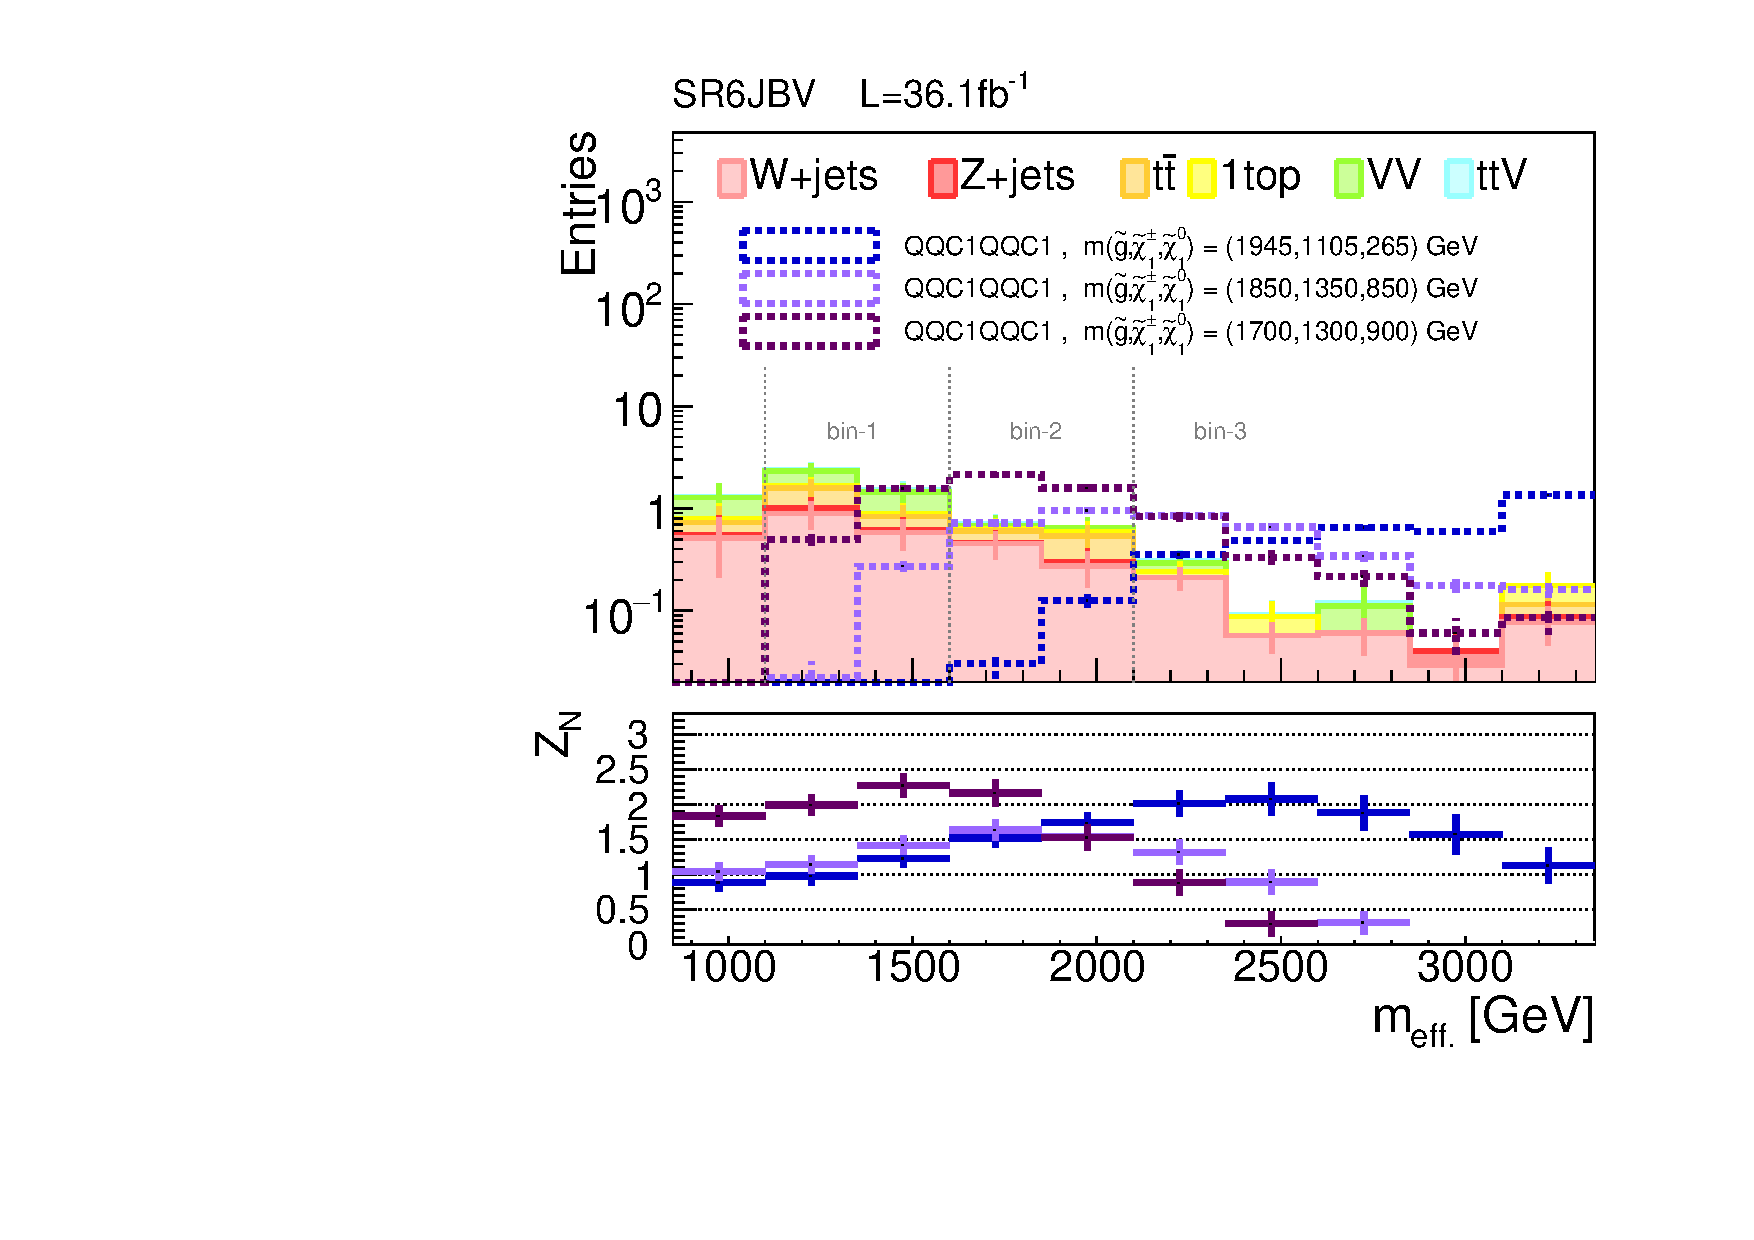
\includegraphics[width=0.45\textwidth]{figures/SRdefinition/N1plot/meffInc30_6JMEFFInclBV.pdf}}
    \subfigure[]{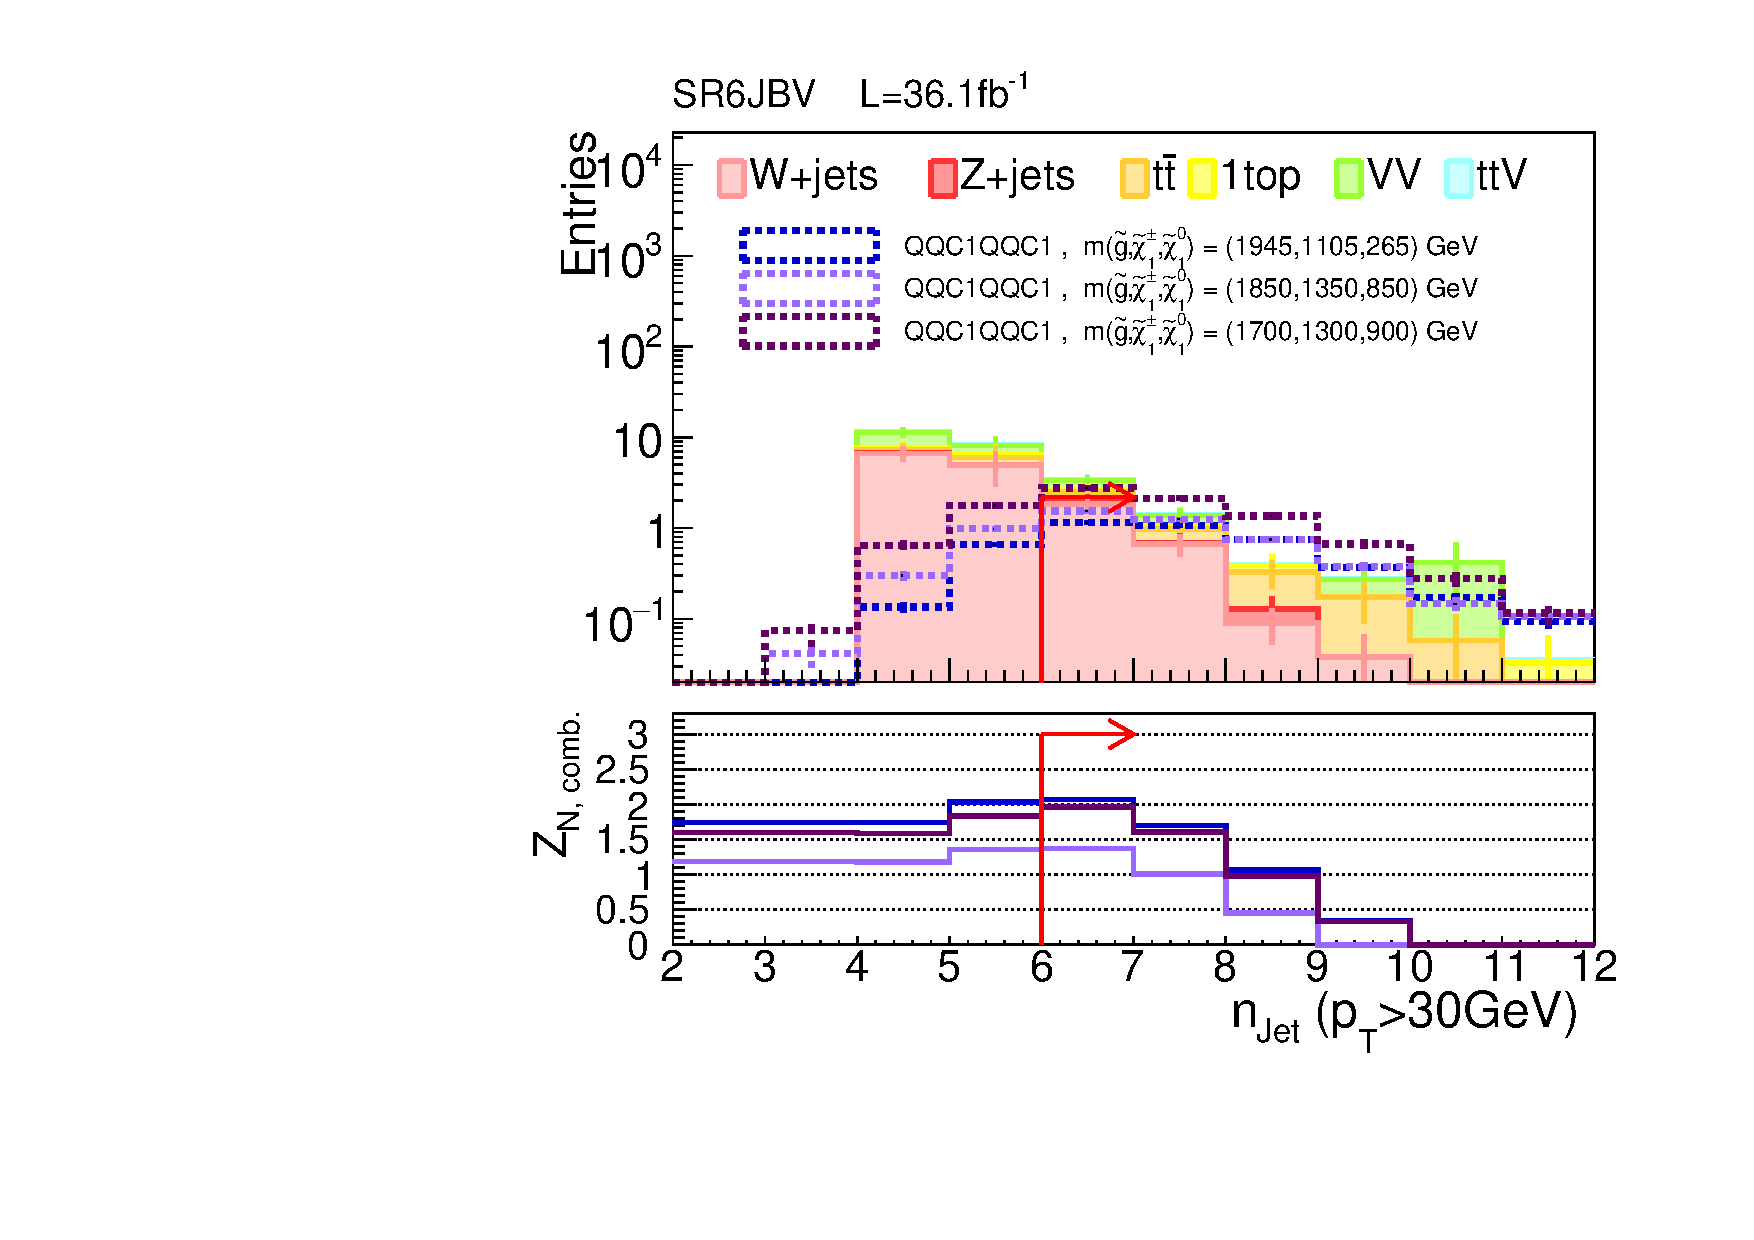
\includegraphics[width=0.45\textwidth]{figures/SRdefinition/N1plot/nJet30_6JMEFFInclBV.pdf}}
    \subfigure[]{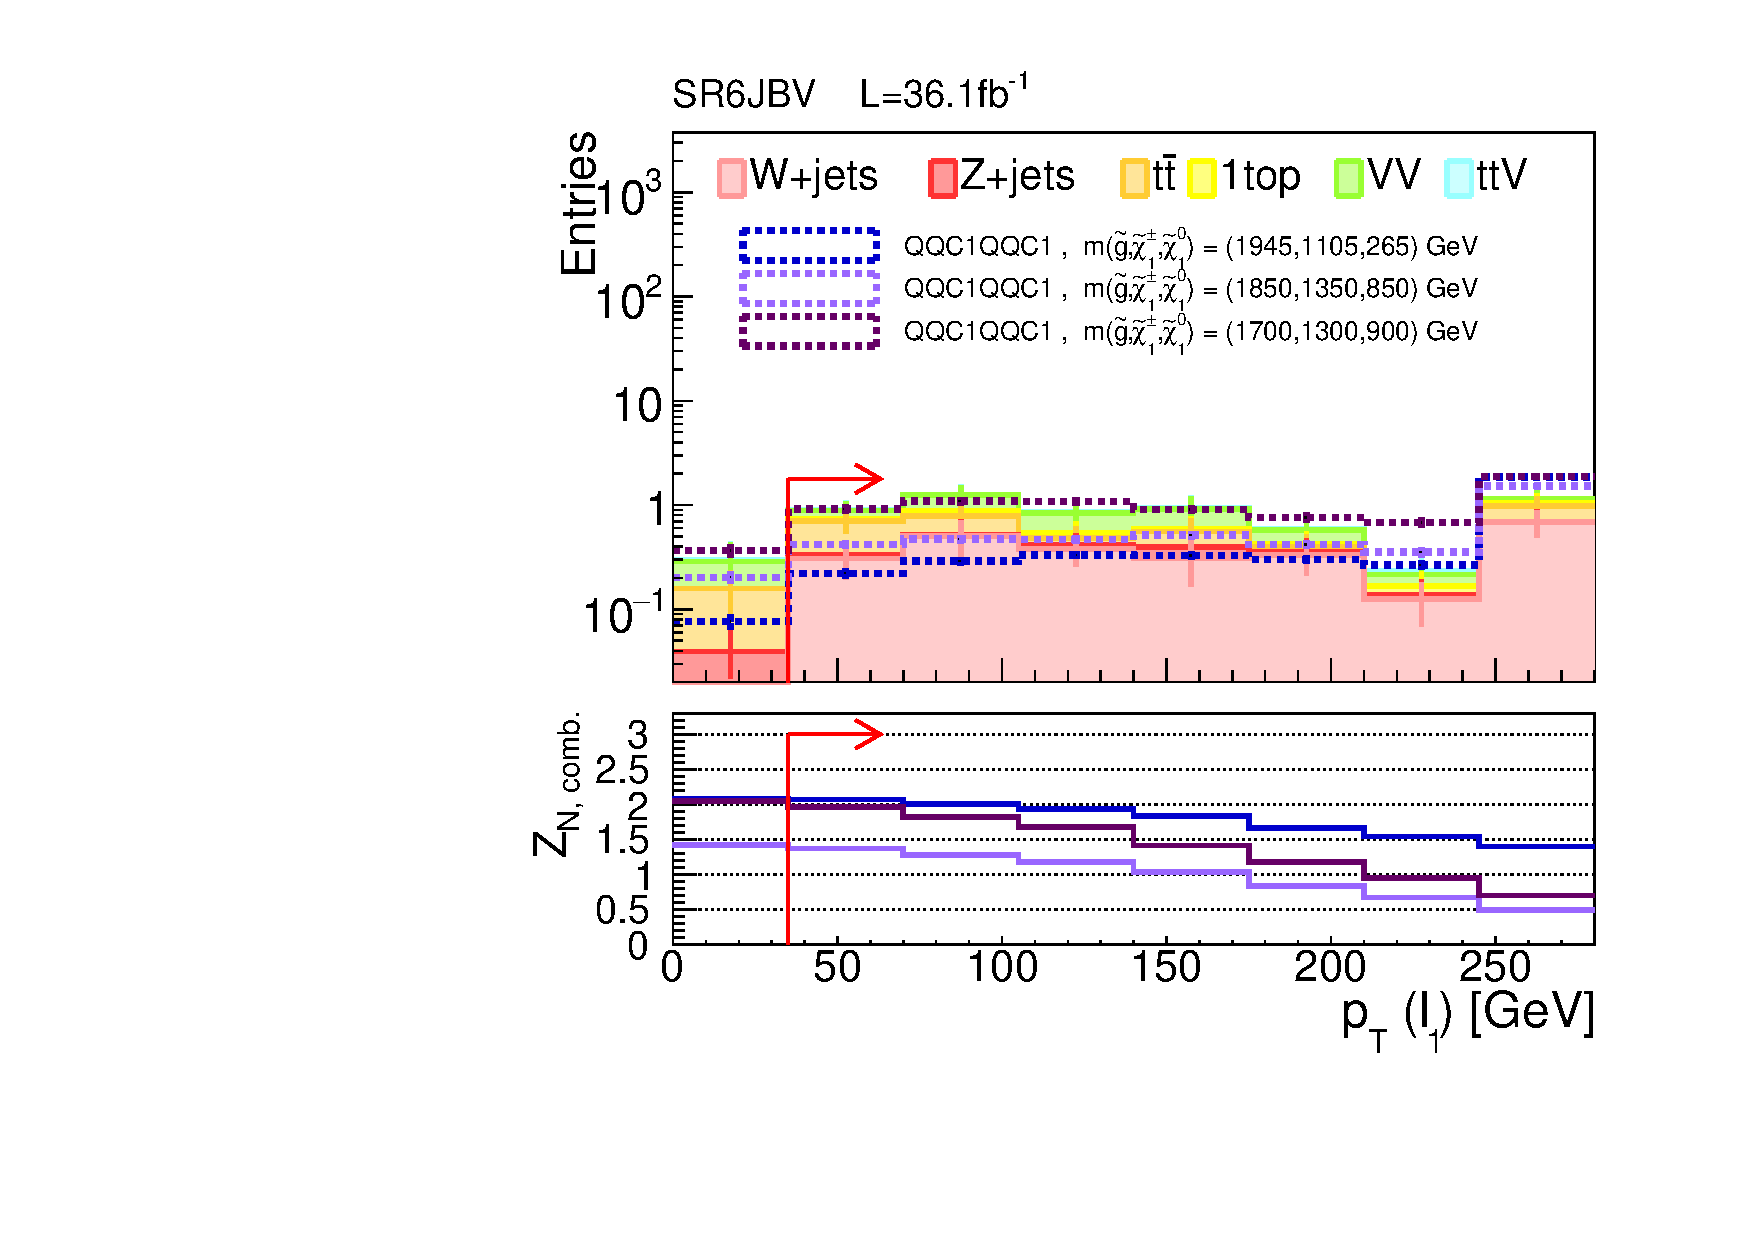
\includegraphics[width=0.45\textwidth]{figures/SRdefinition/N1plot/lep1Pt_6JMEFFInclBV.pdf}}
    \subfigure[]{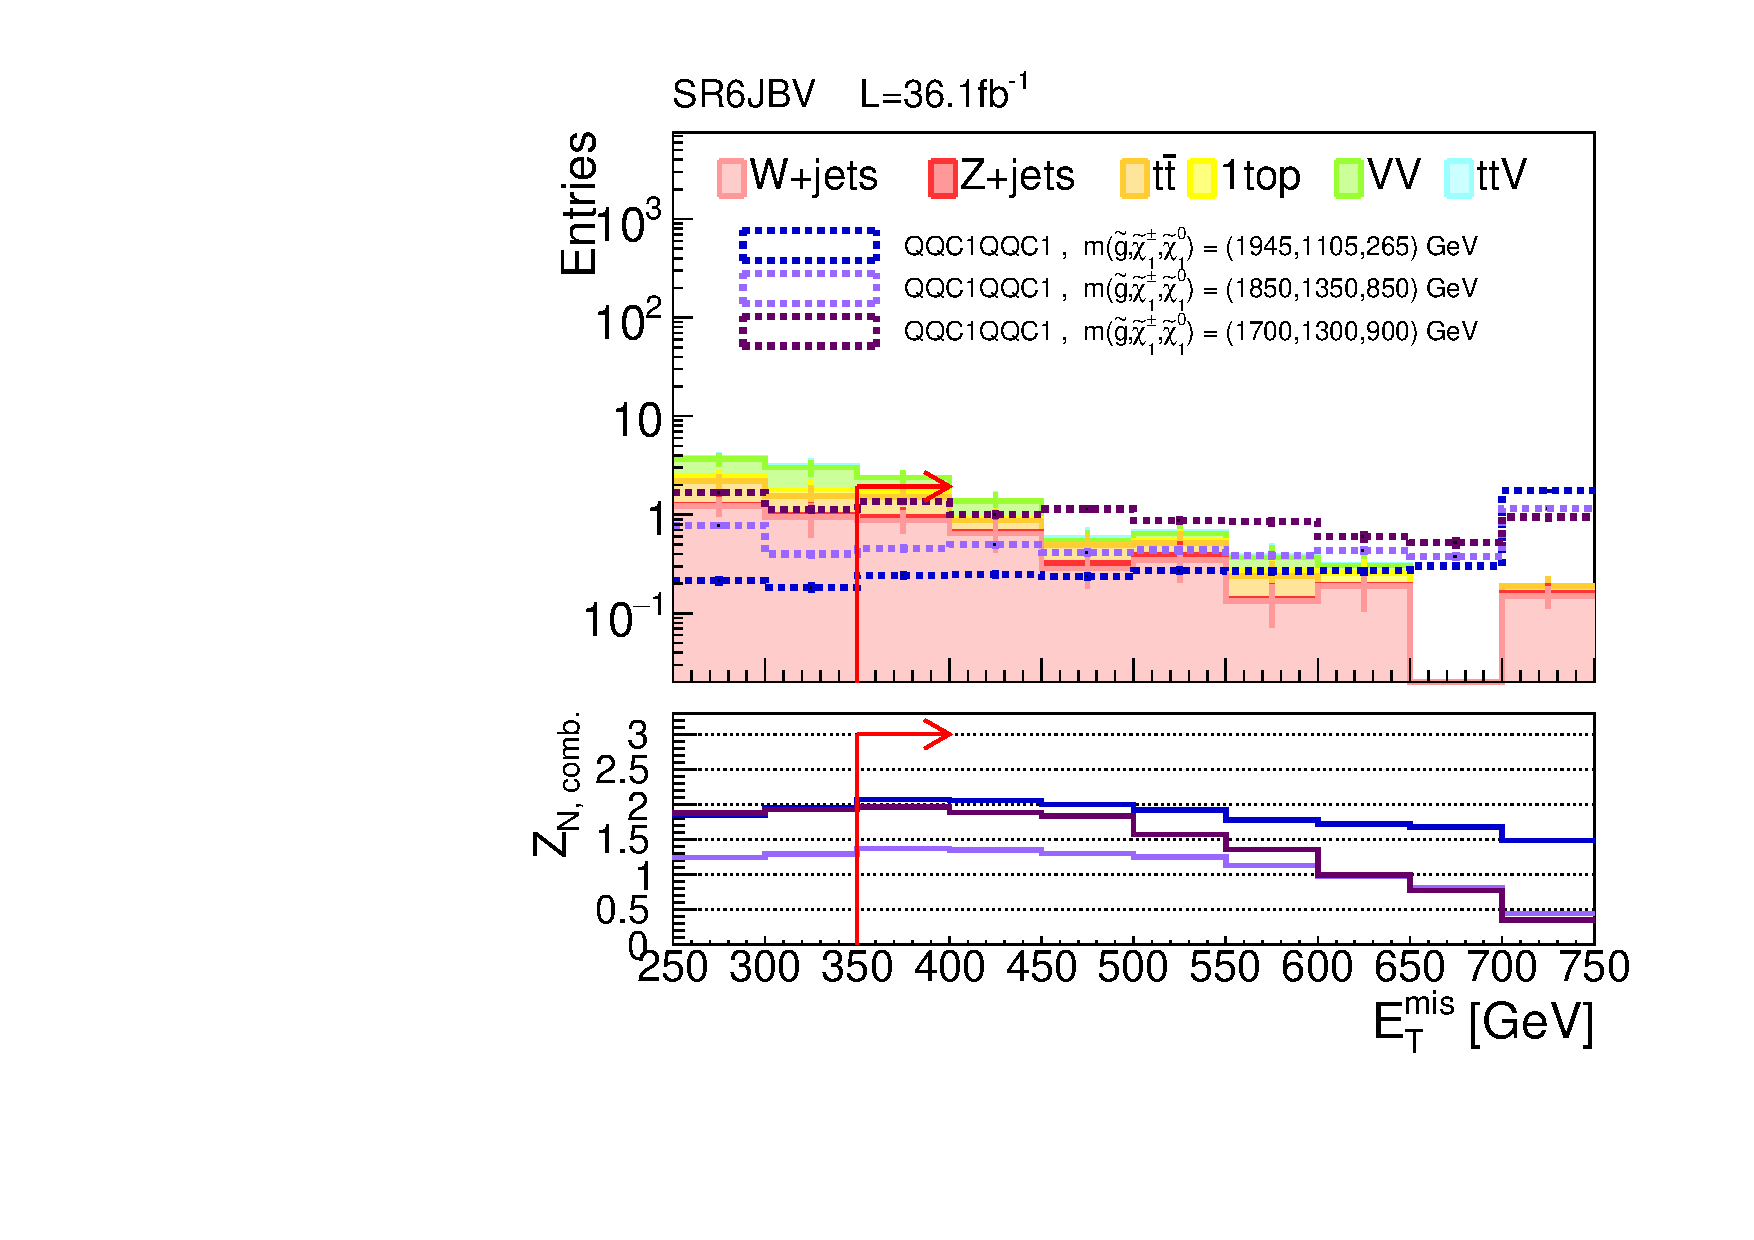
\includegraphics[width=0.45\textwidth]{figures/SRdefinition/N1plot/met_6JMEFFInclBV.pdf}}
    \subfigure[]{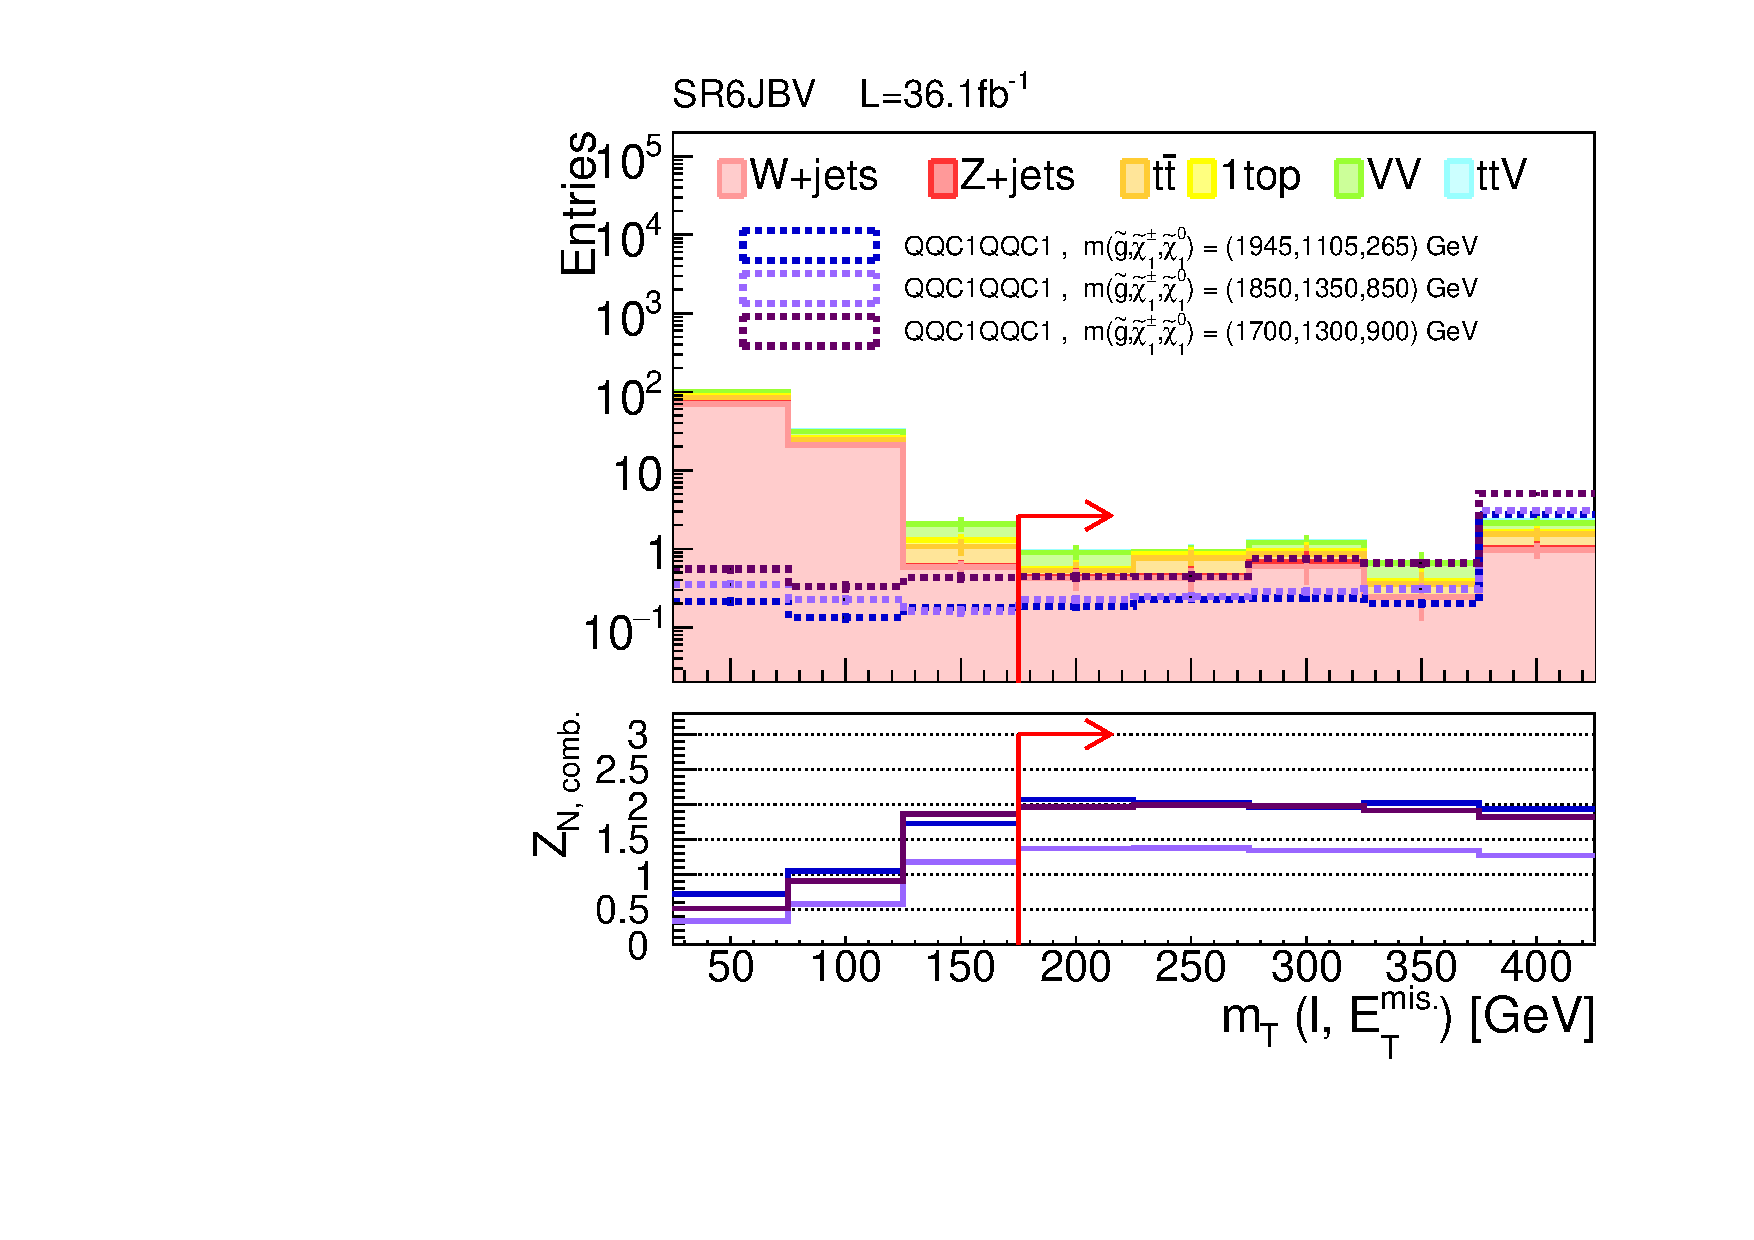
\includegraphics[width=0.45\textwidth]{figures/SRdefinition/N1plot/mt_6JMEFFInclBV.pdf}}
    \subfigure[]{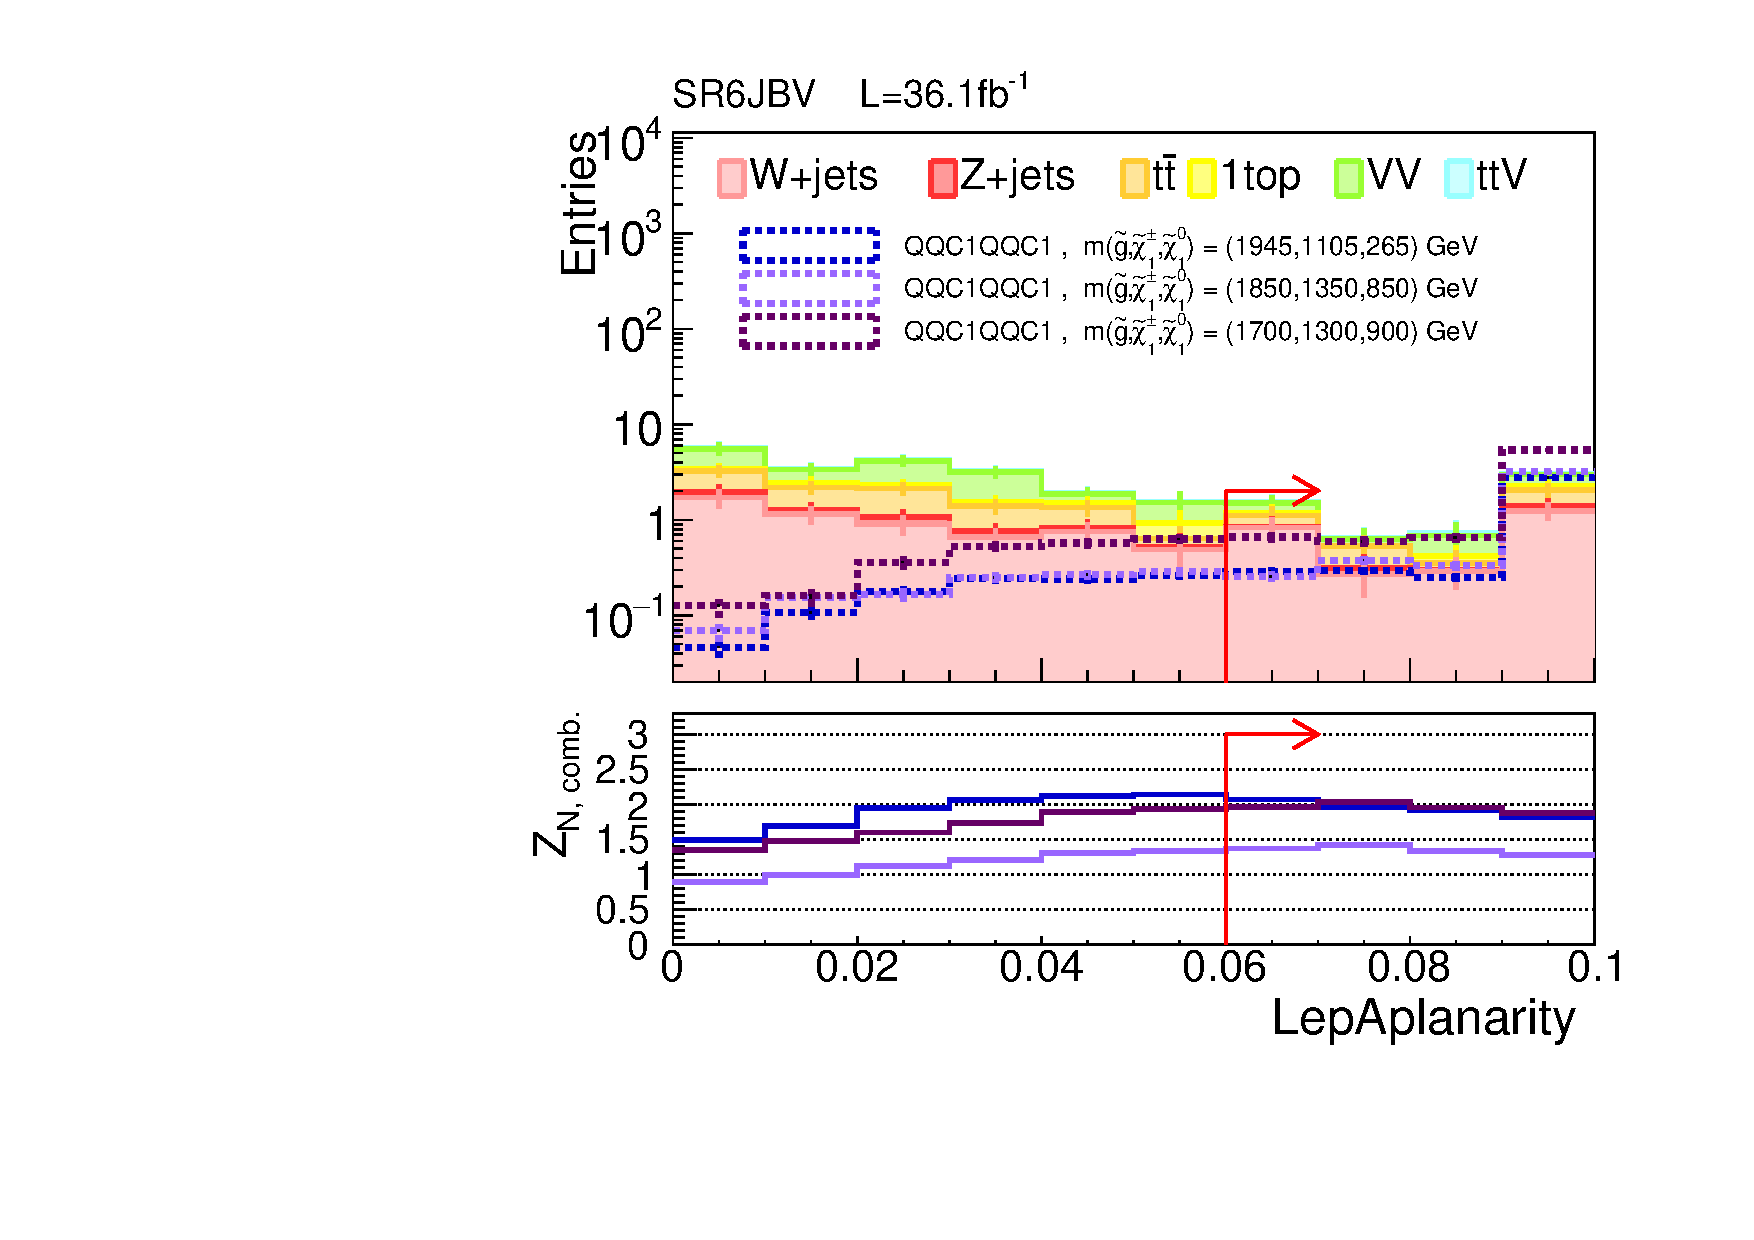
\includegraphics[width=0.45\textwidth]{figures/SRdefinition/N1plot/LepAplanarity_6JMEFFInclBV.pdf}}
    \subfigure[]{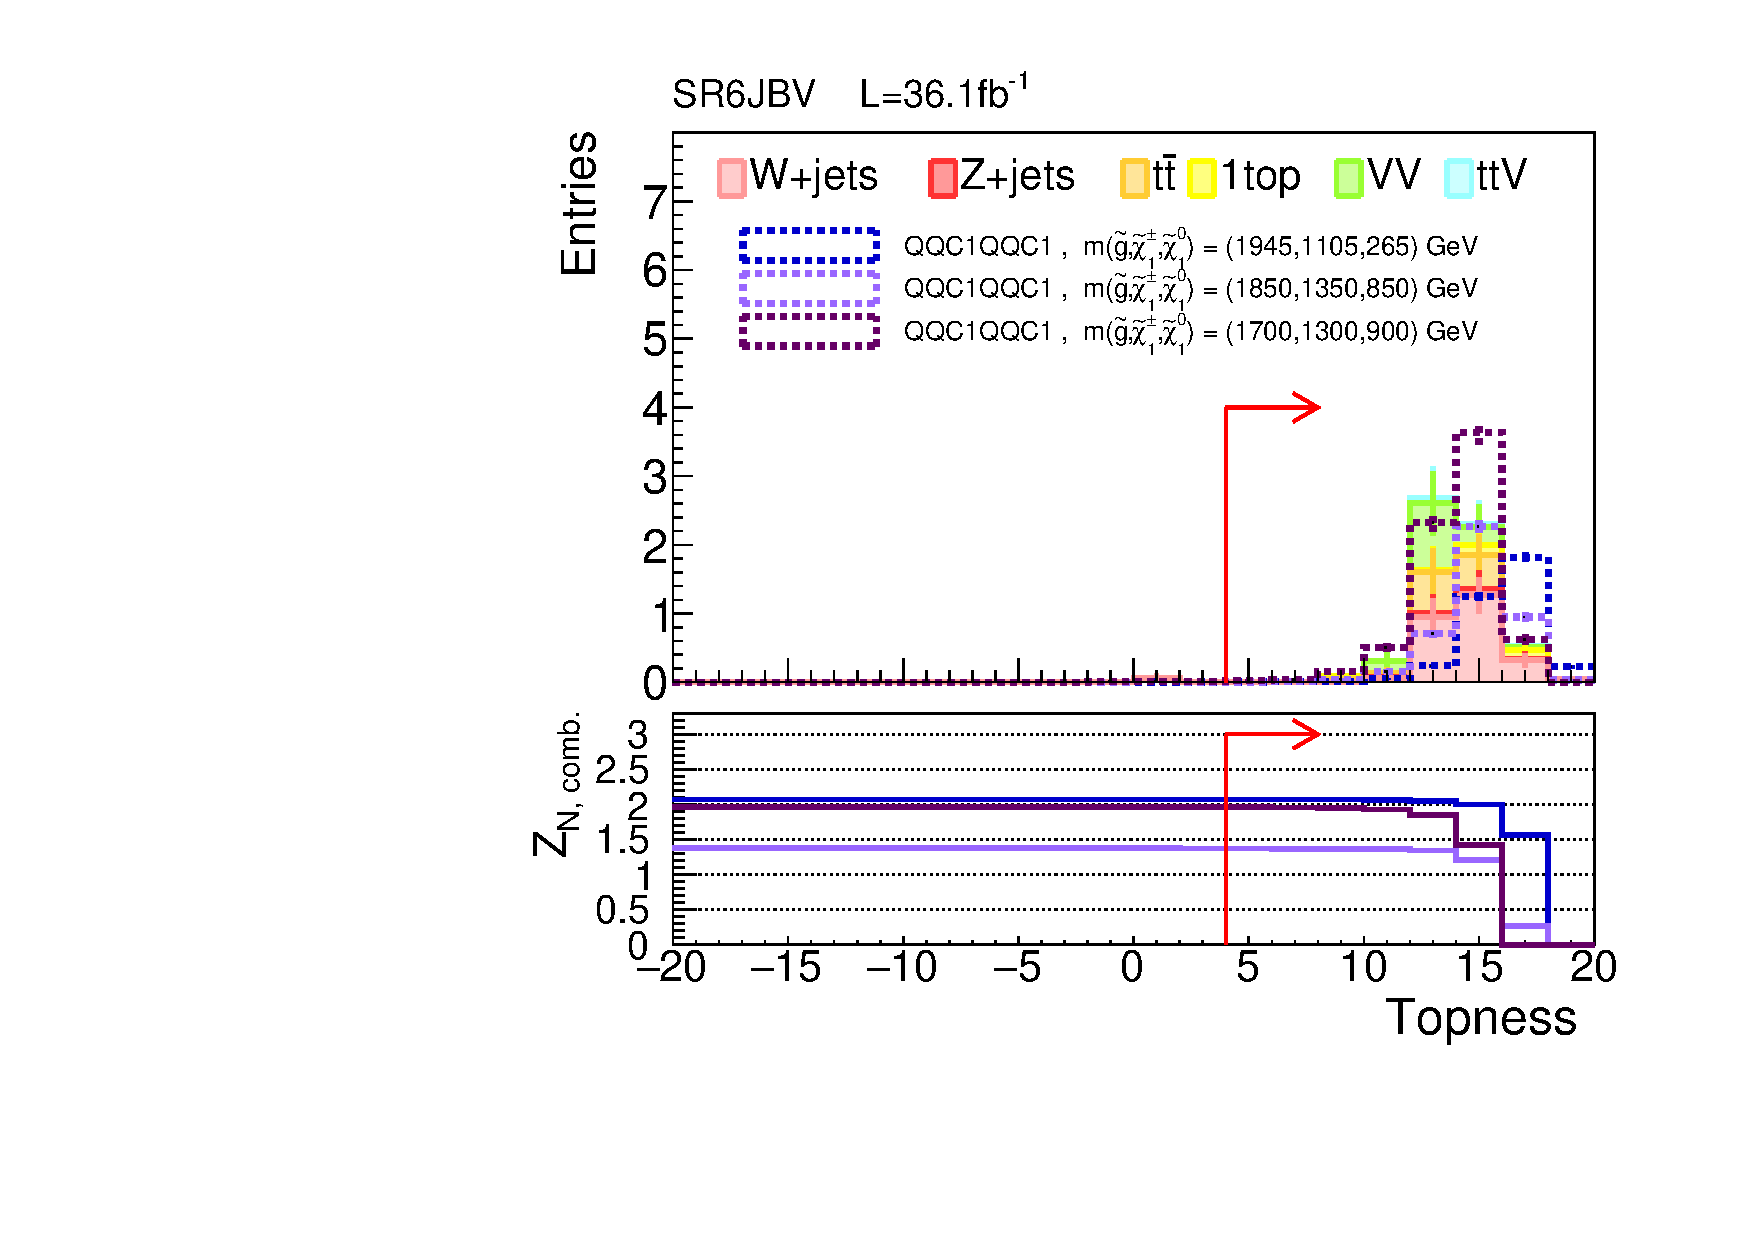
\includegraphics[width=0.45\textwidth]{figures/SRdefinition/N1plot/topNess_6JMEFFInclBV.pdf}}
    \caption{ 
    N-1 plots for the b-vetoed (BV) slices of the optimized \textbf{6J} signal regions.
    Bottom row presents the combined significace over the $\meffInc$ bins defined in Eq. \ref{ZNcomb}.
        \label{fig::SRdefinition::N1plots_6JMEFFInclBV}
        }       
\end{figure}
 

\clearpage
\begin{figure}[h]
  \centering
 %   \subfigure[]{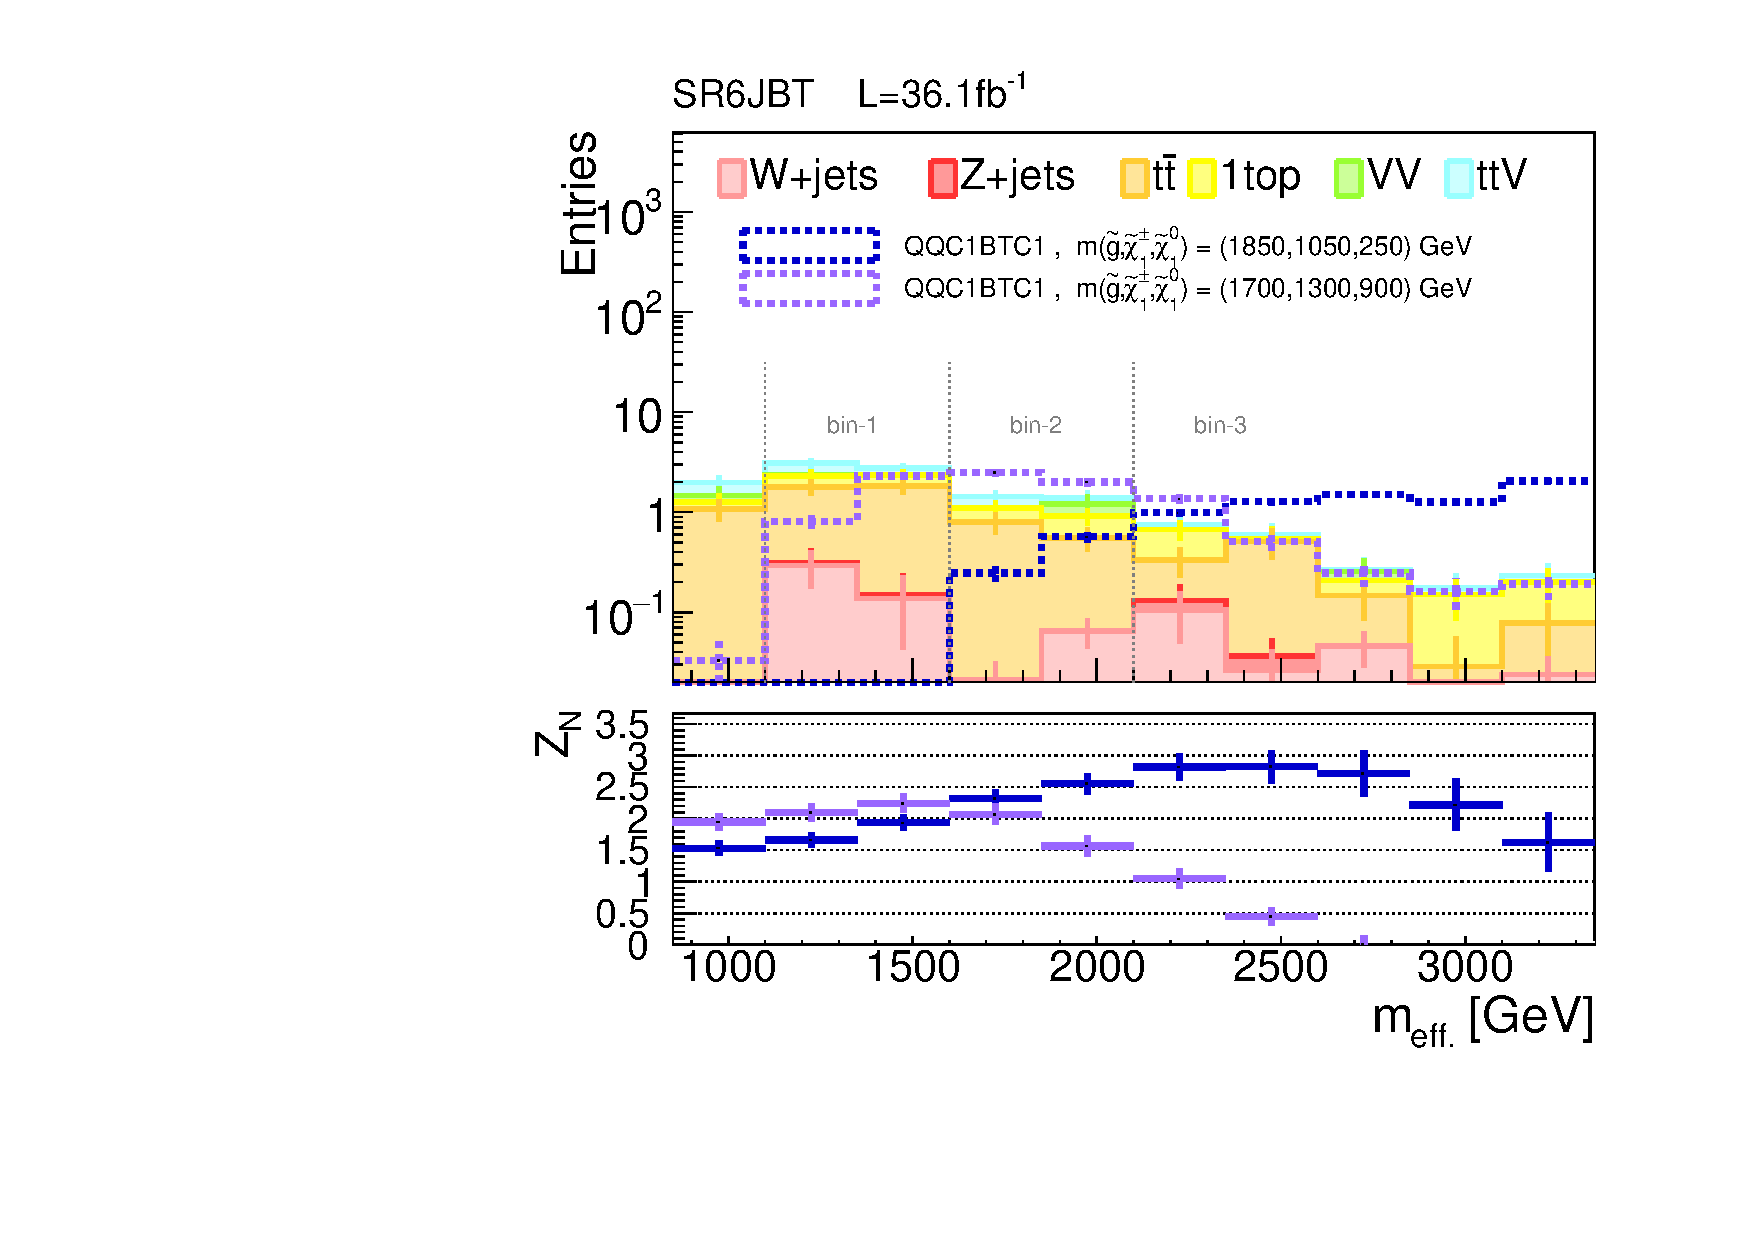
\includegraphics[width=0.45\textwidth]{figures/SRdefinition/N1plot/meffInc30_6JMEFFInclBT.pdf}}
    \subfigure[]{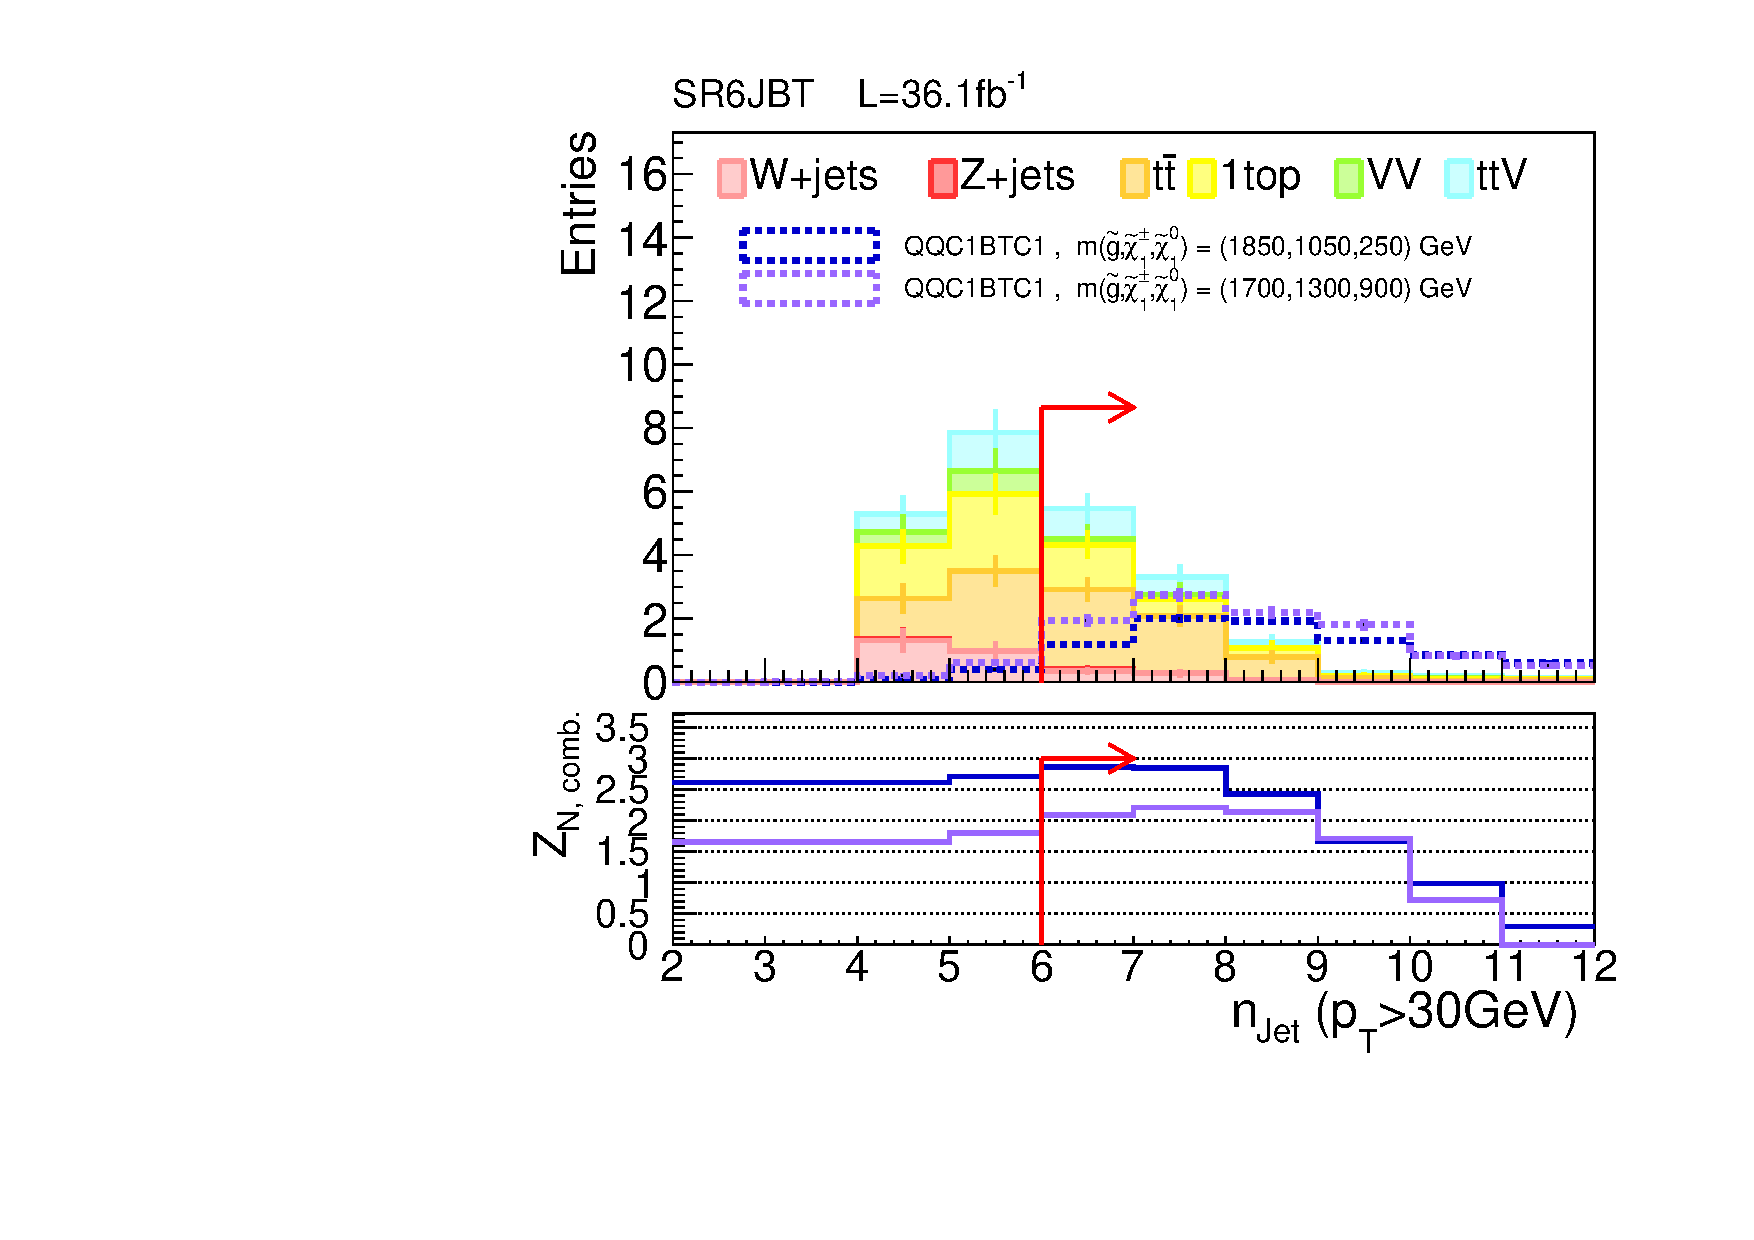
\includegraphics[width=0.45\textwidth]{figures/SRdefinition/N1plot/nJet30_6JMEFFInclBT.pdf}}
    \subfigure[]{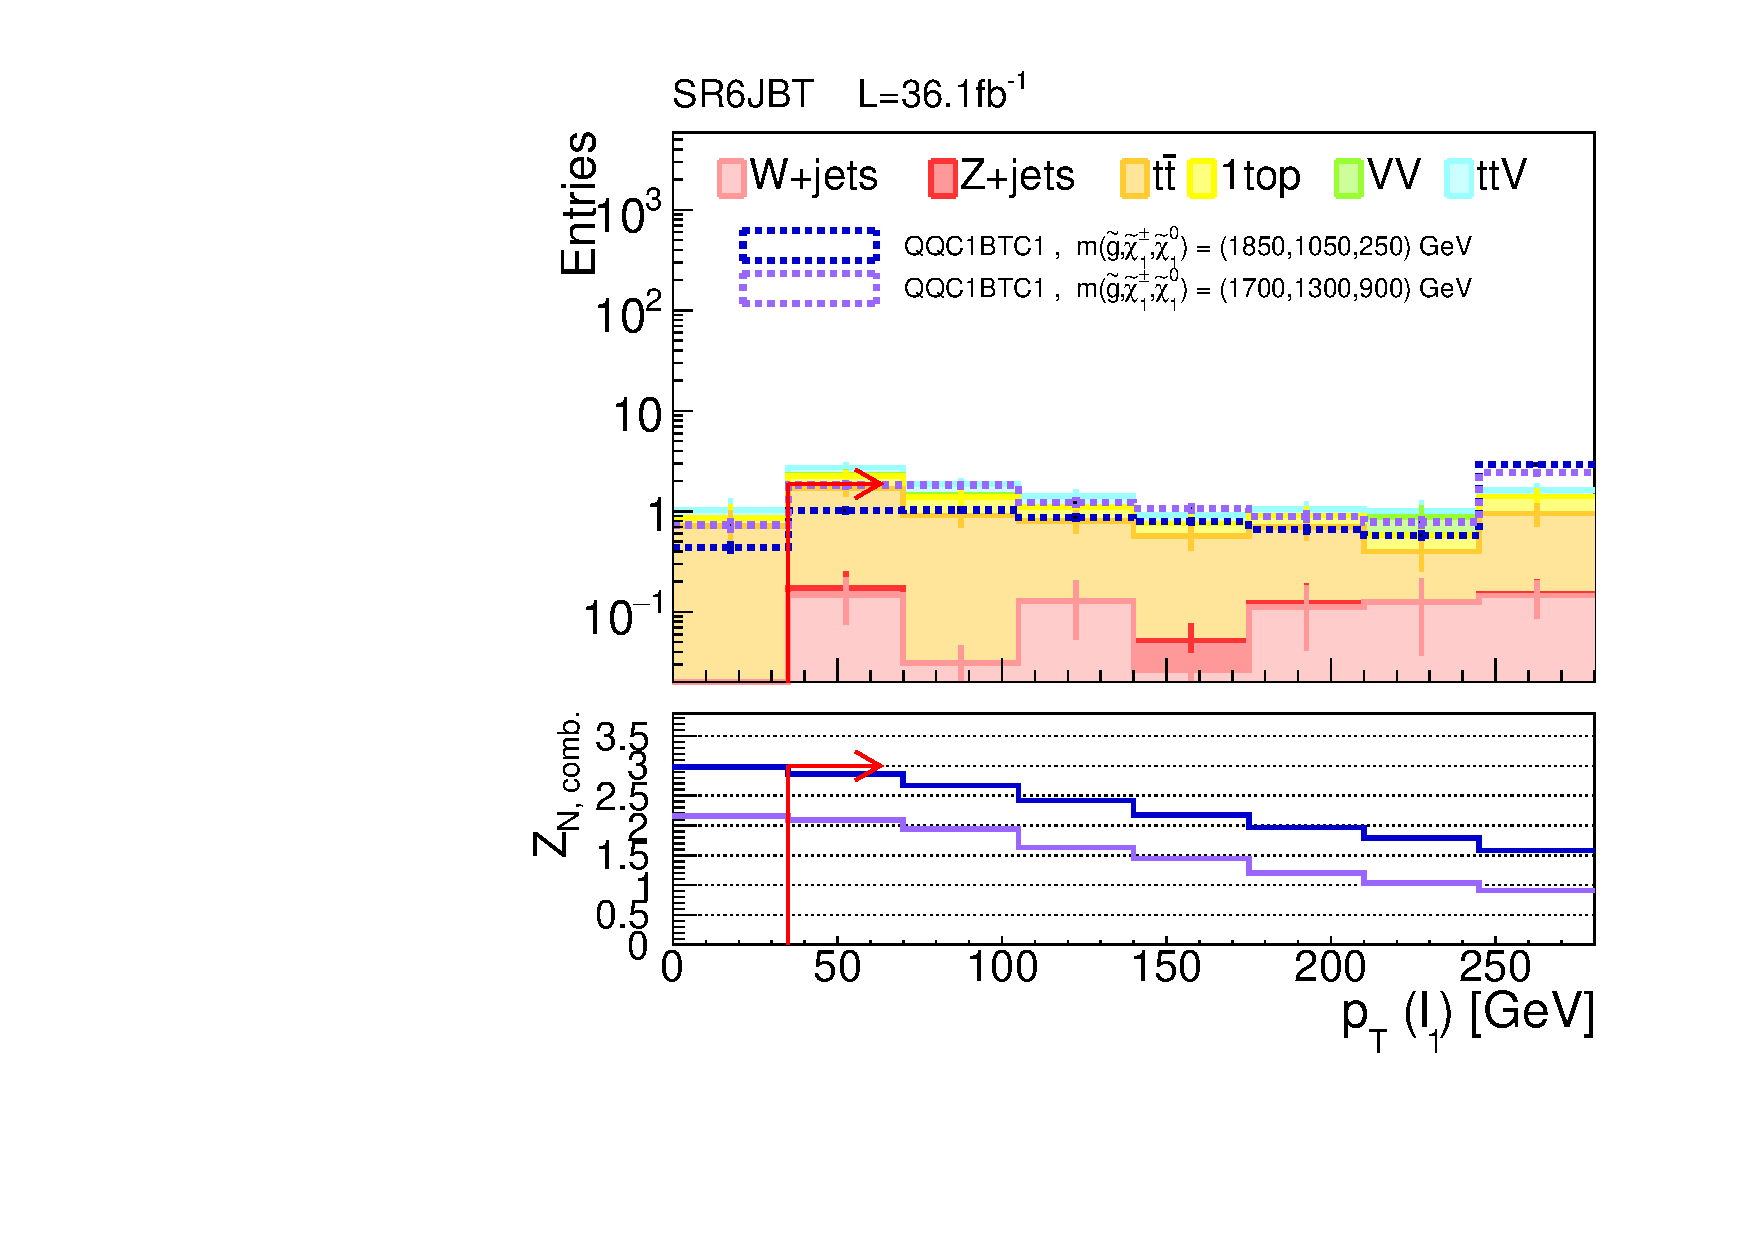
\includegraphics[width=0.45\textwidth]{figures/SRdefinition/N1plot/lep1Pt_6JMEFFInclBT.pdf}}
    \subfigure[]{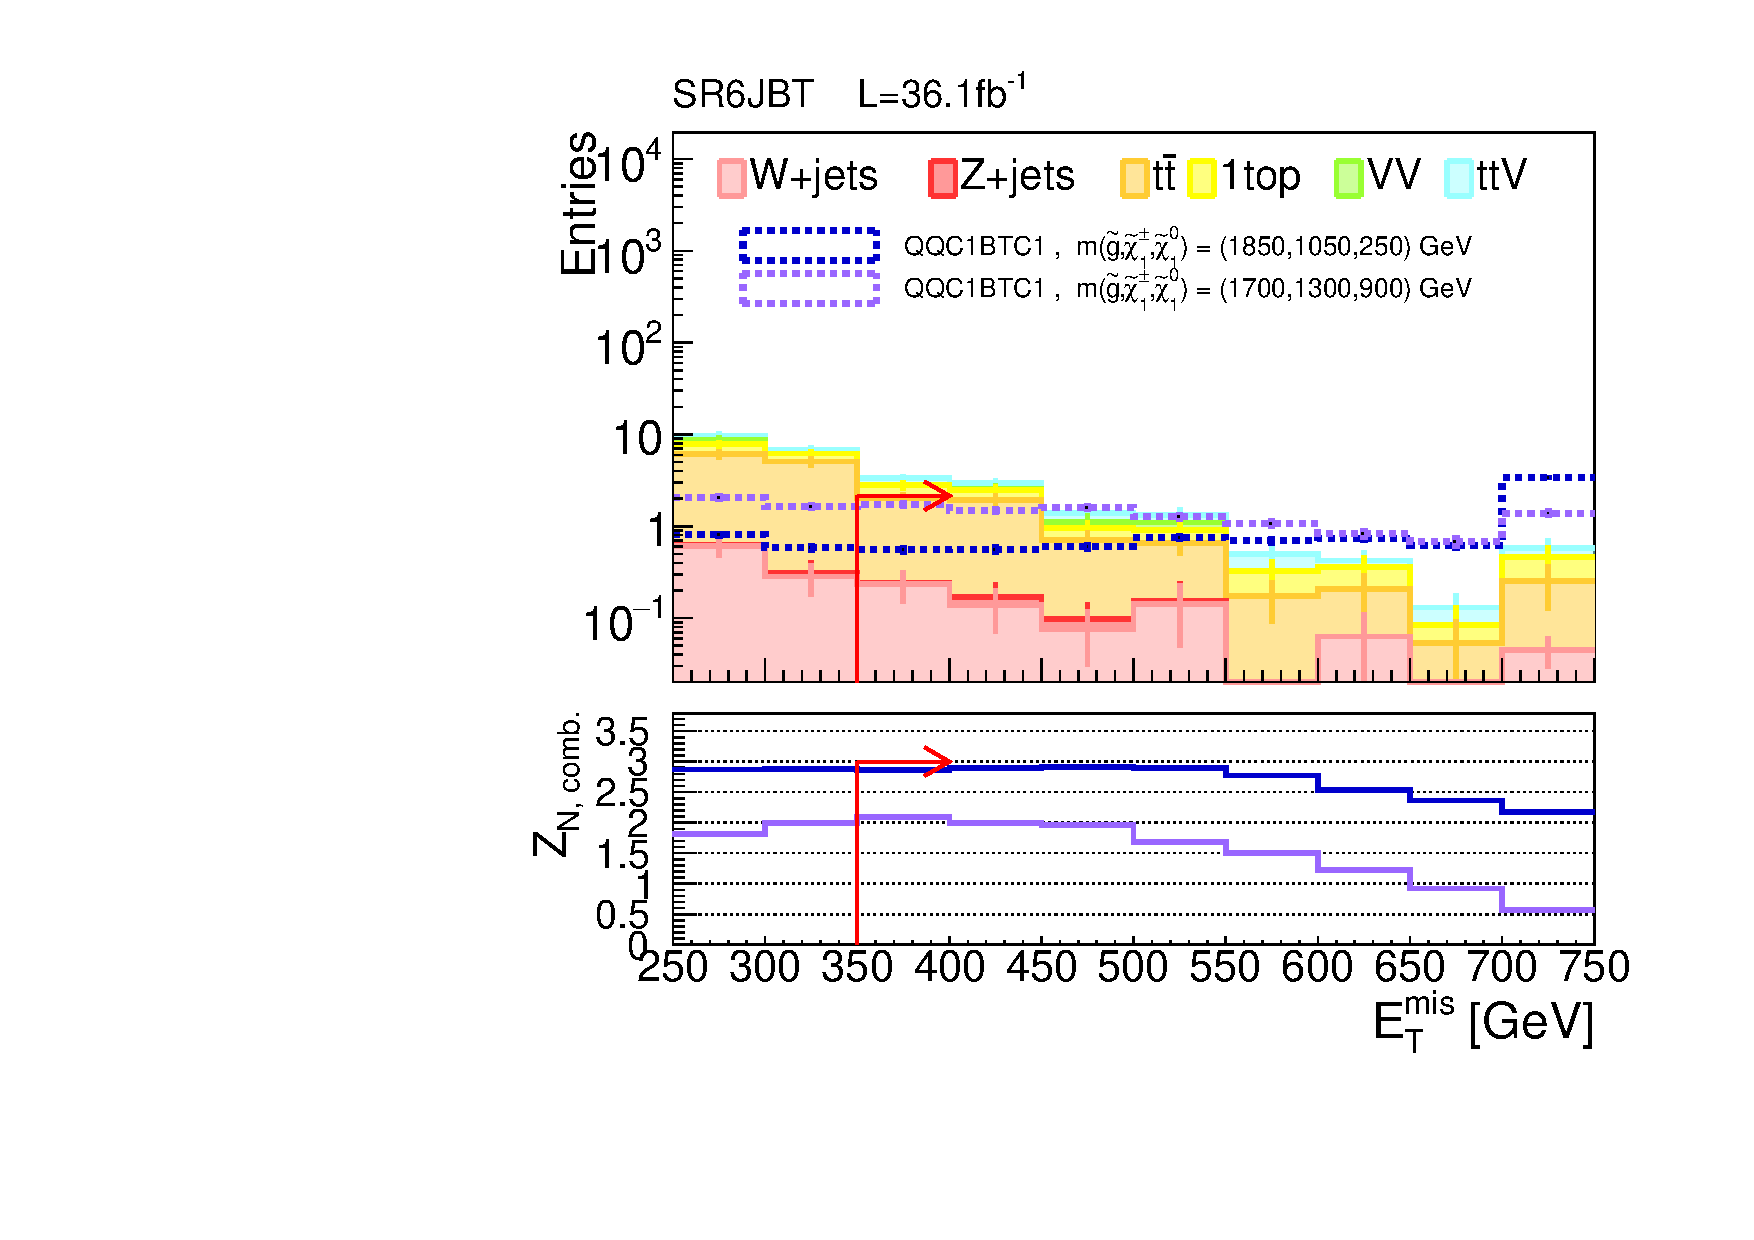
\includegraphics[width=0.45\textwidth]{figures/SRdefinition/N1plot/met_6JMEFFInclBT.pdf}}
    \subfigure[]{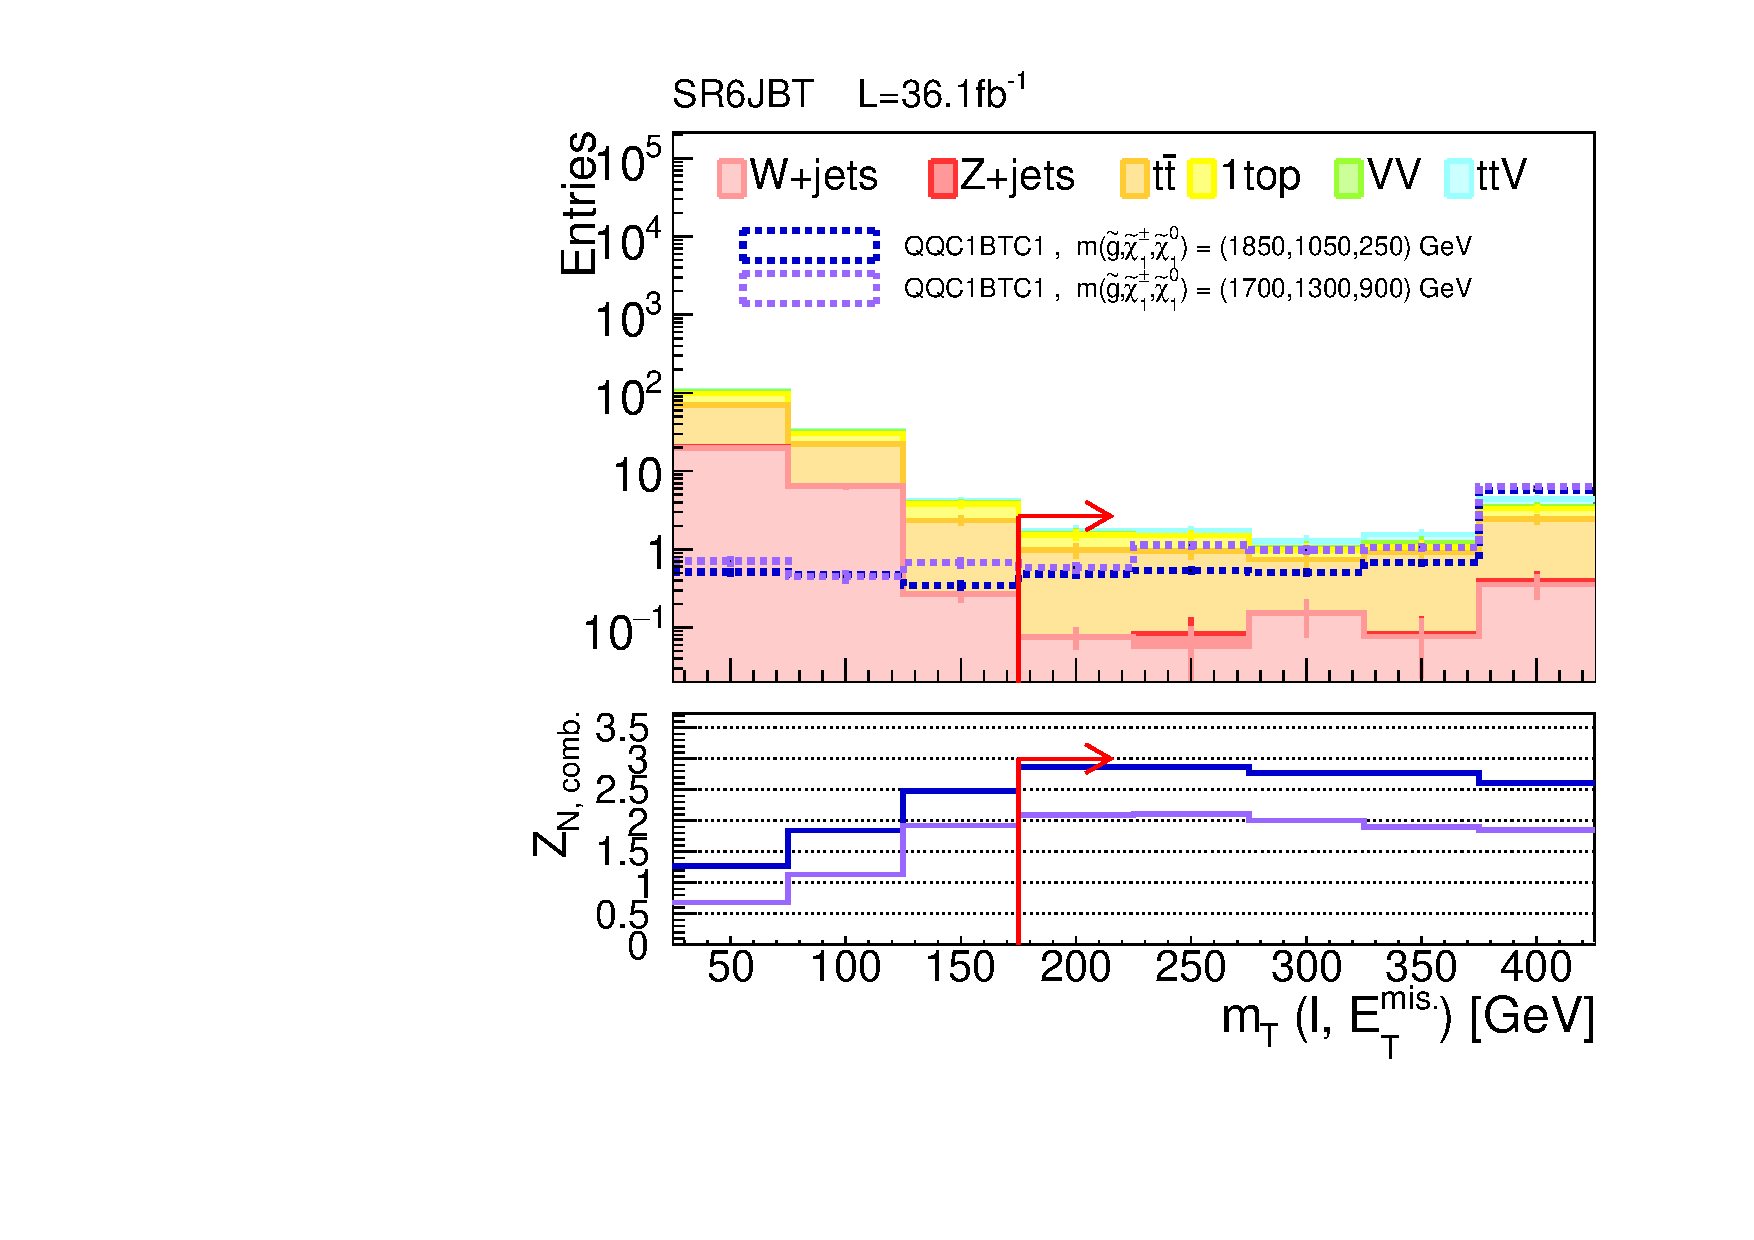
\includegraphics[width=0.45\textwidth]{figures/SRdefinition/N1plot/mt_6JMEFFInclBT.pdf}}
    \subfigure[]{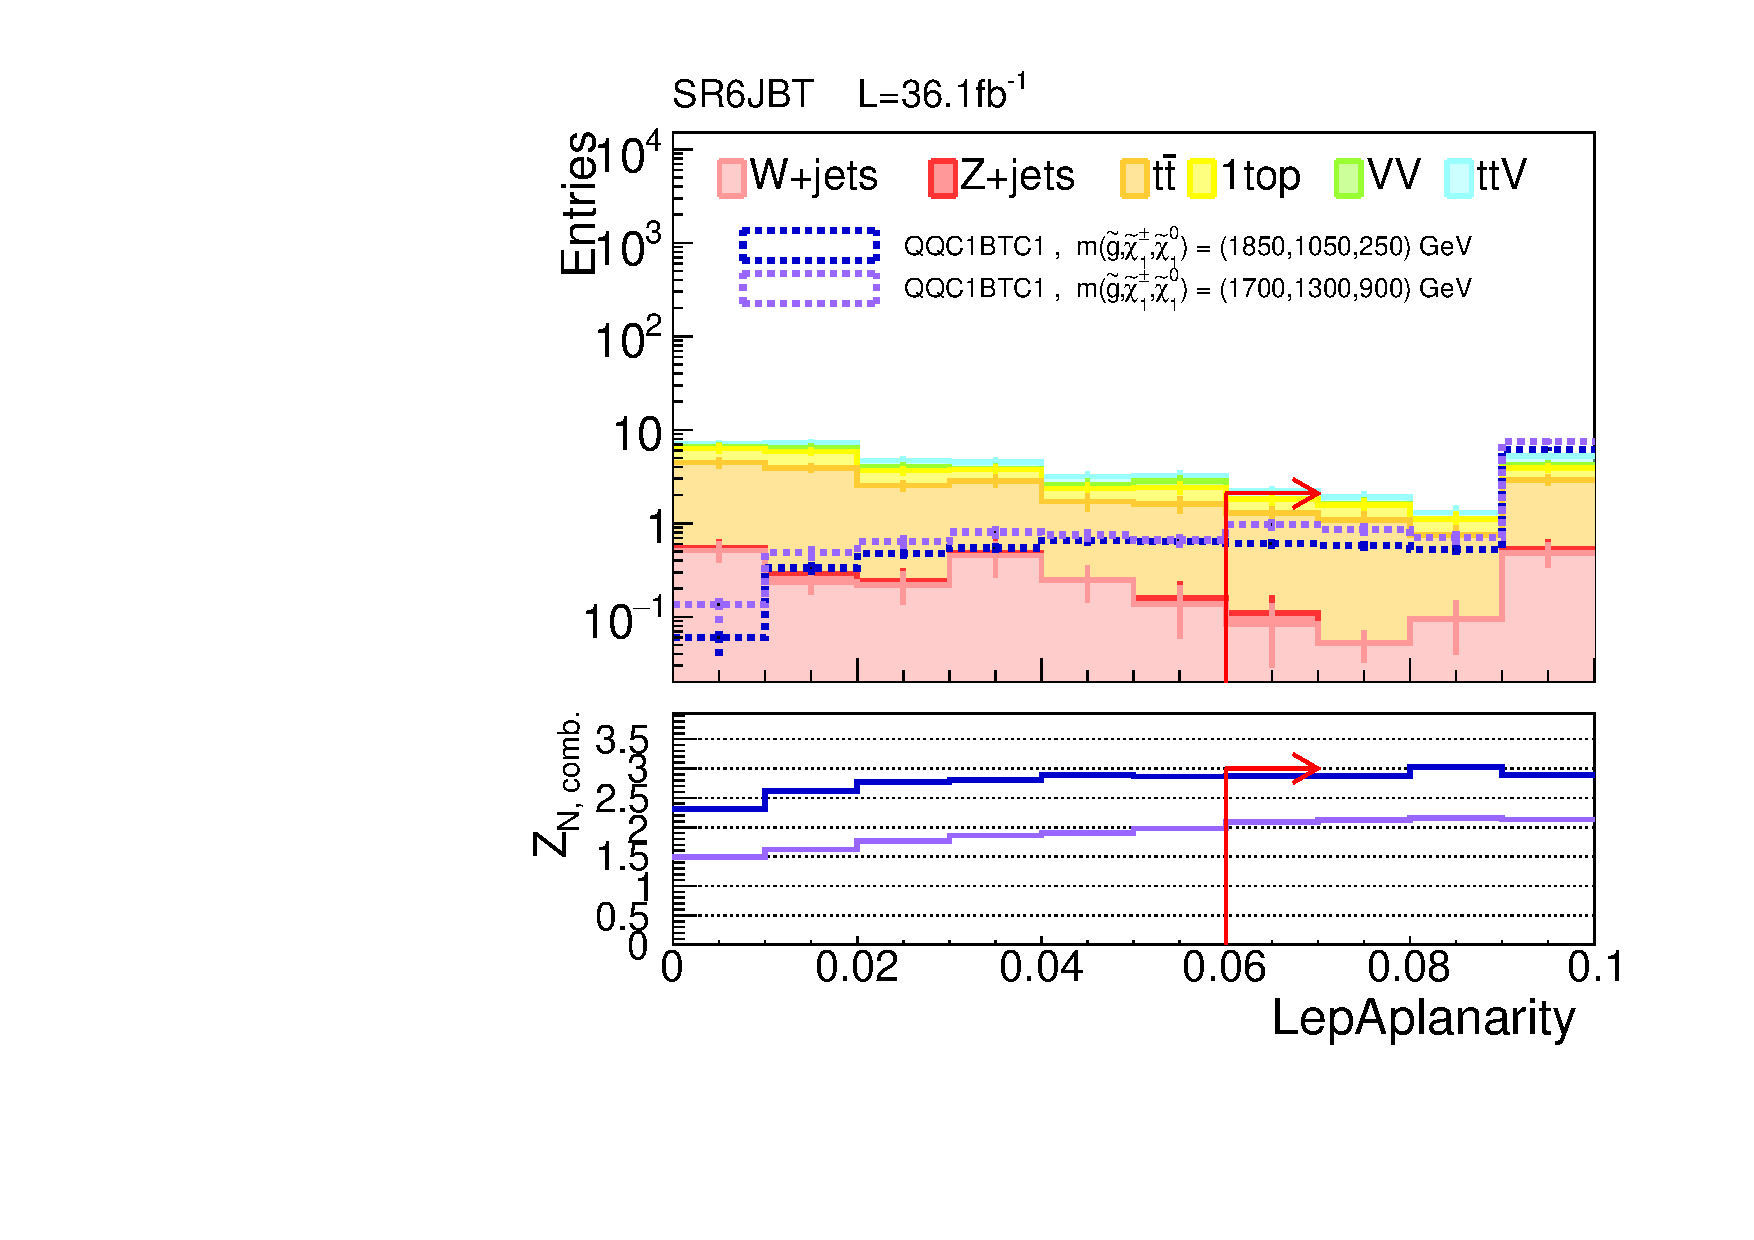
\includegraphics[width=0.45\textwidth]{figures/SRdefinition/N1plot/LepAplanarity_6JMEFFInclBT.pdf}}
    \subfigure[]{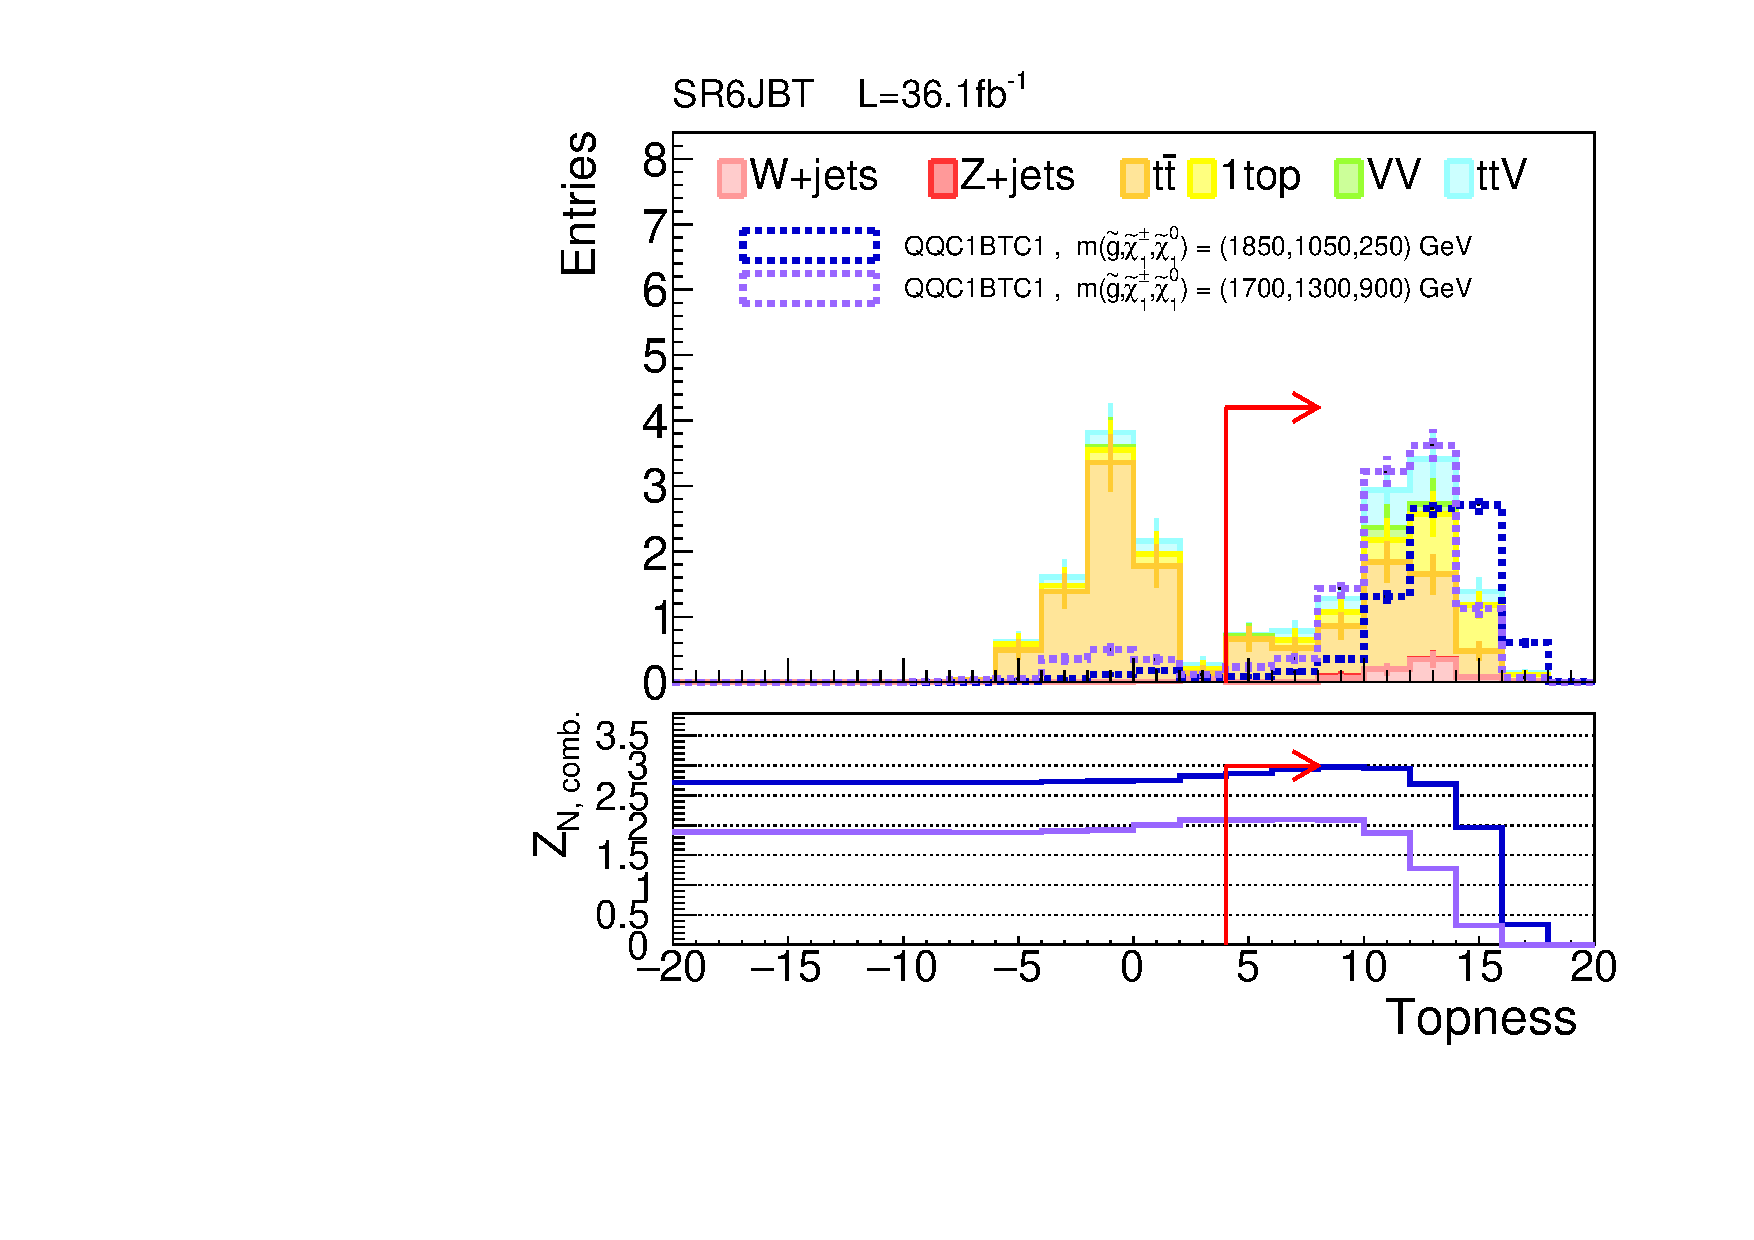
\includegraphics[width=0.45\textwidth]{figures/SRdefinition/N1plot/topNess_6JMEFFInclBT.pdf}}
    \caption{ 
    N-1 plots for the b-tagged (BT) slices of the optimized \textbf{6J} signal regions.
    Bottom row presents the combined significace over the $\meffInc$ bins defined in Eq. \ref{ZNcomb}.
        \label{fig::SRdefinition::N1plots_6JMEFFInclBT} 
    }
\end{figure}
 

\clearpage
\begin{figure}[h]
  \centering
 %   \subfigure[]{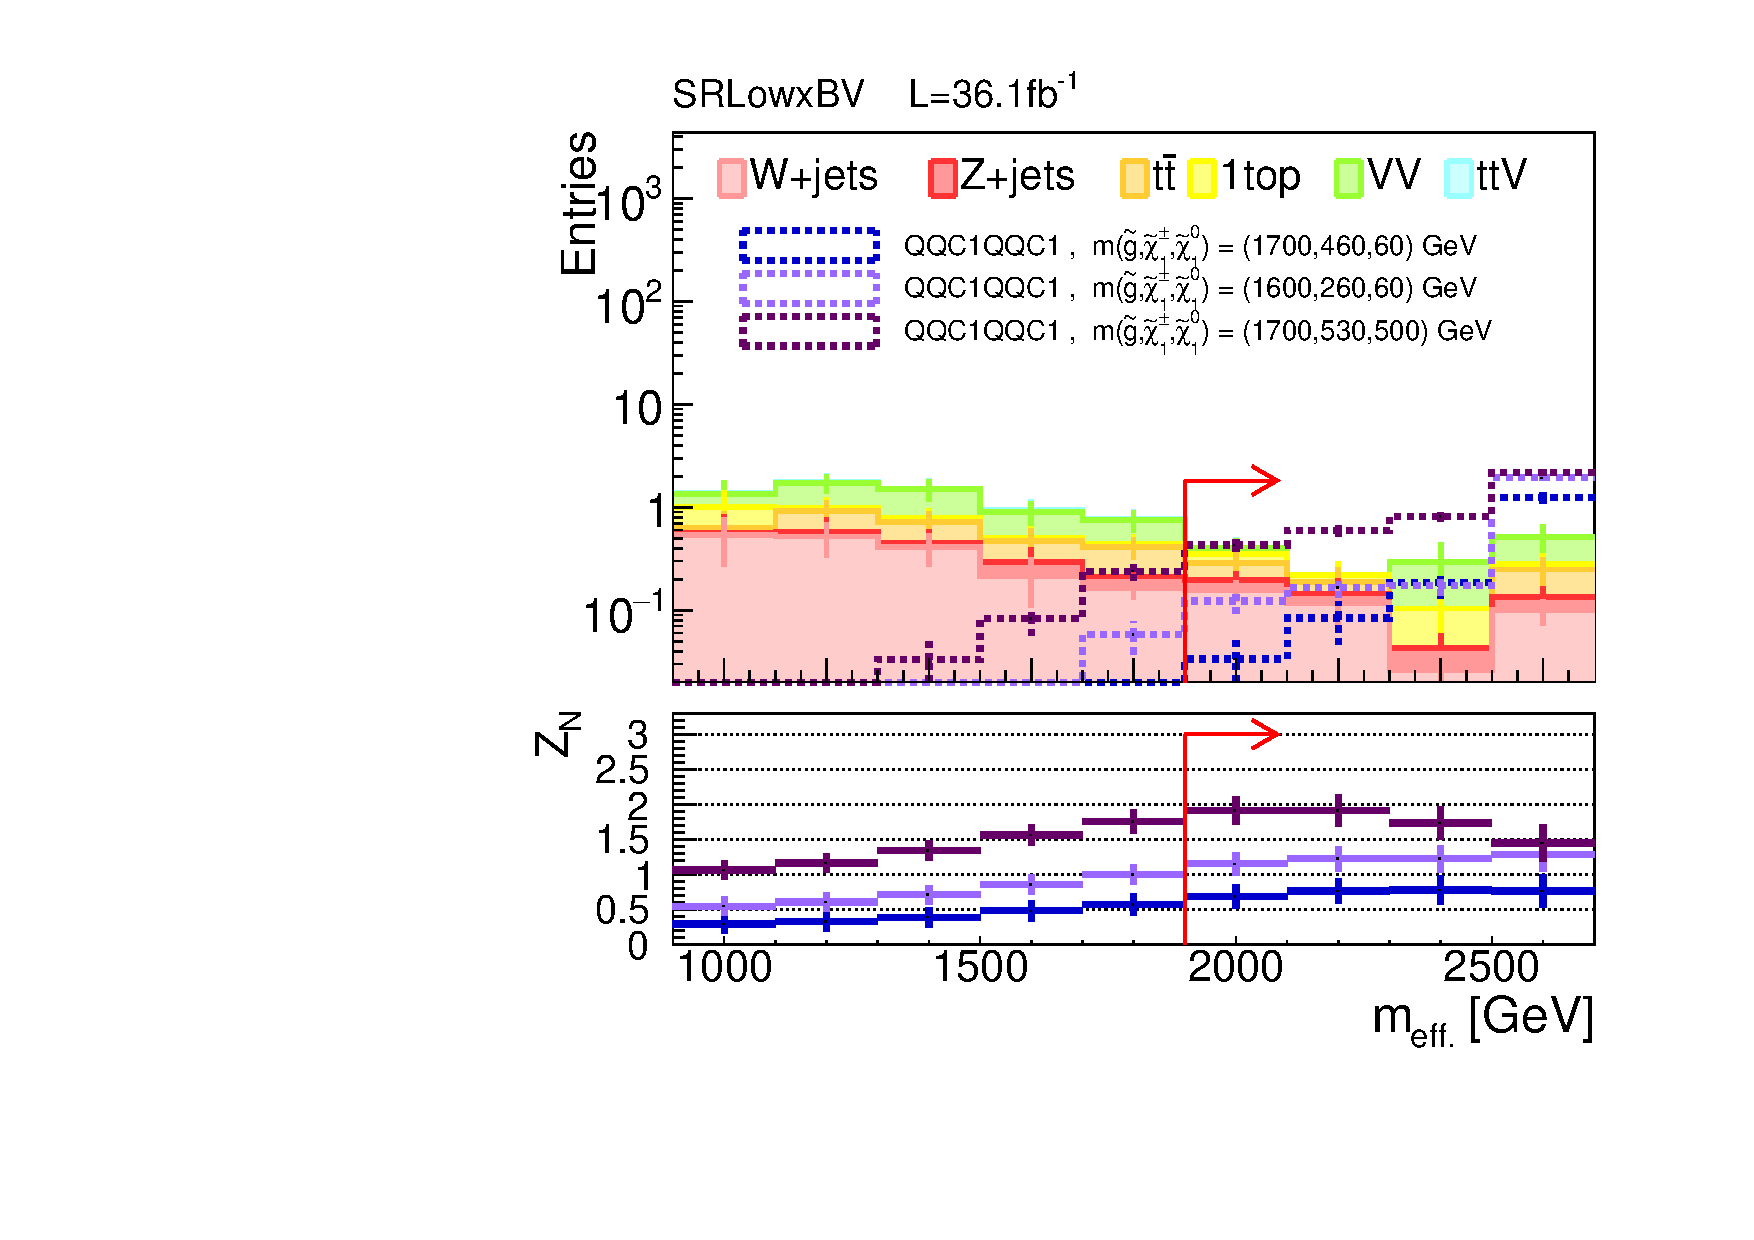
\includegraphics[width=0.45\textwidth]{figures/SRdefinition/N1plot/meffInc30_LowxBV.pdf}}
    \subfigure[]{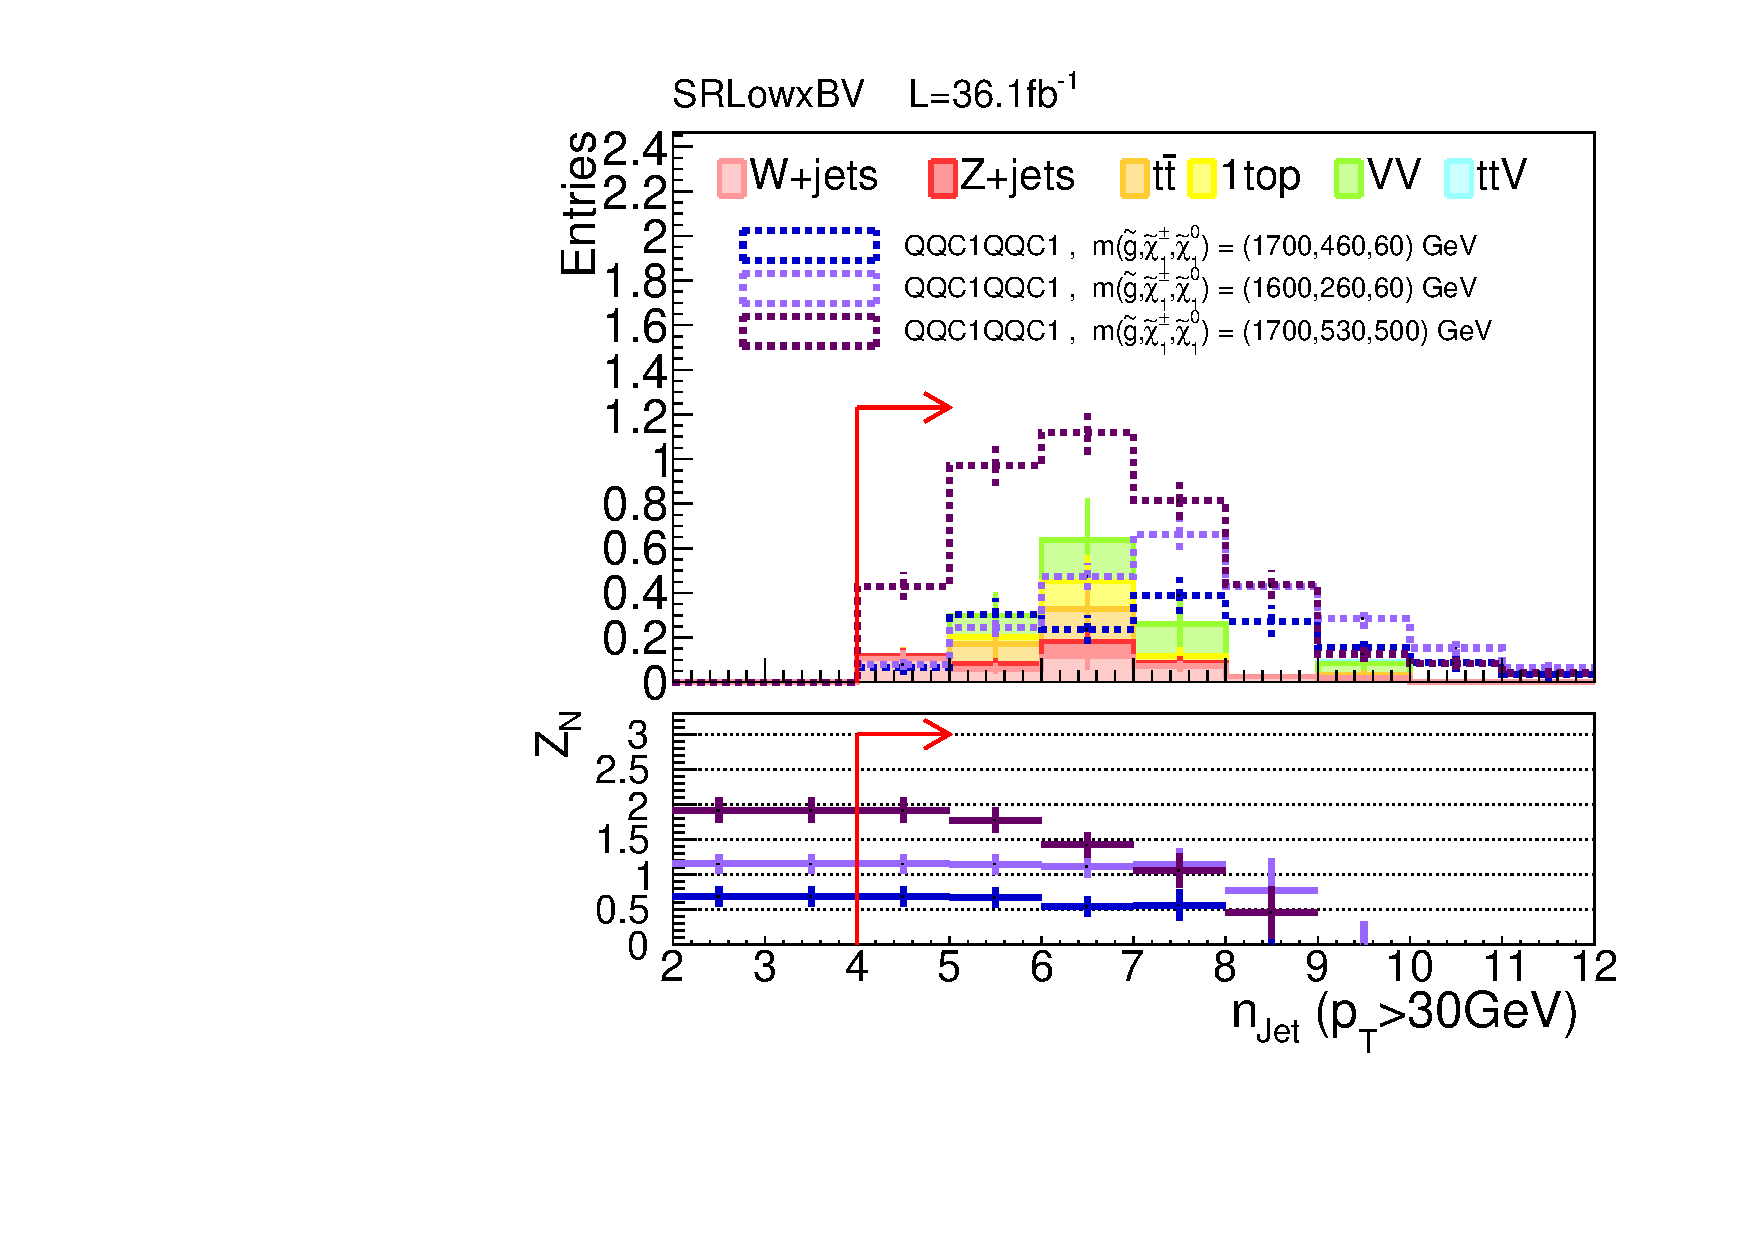
\includegraphics[width=0.45\textwidth]{figures/SRdefinition/N1plot/nJet30_LowxBV.pdf}}
    \subfigure[]{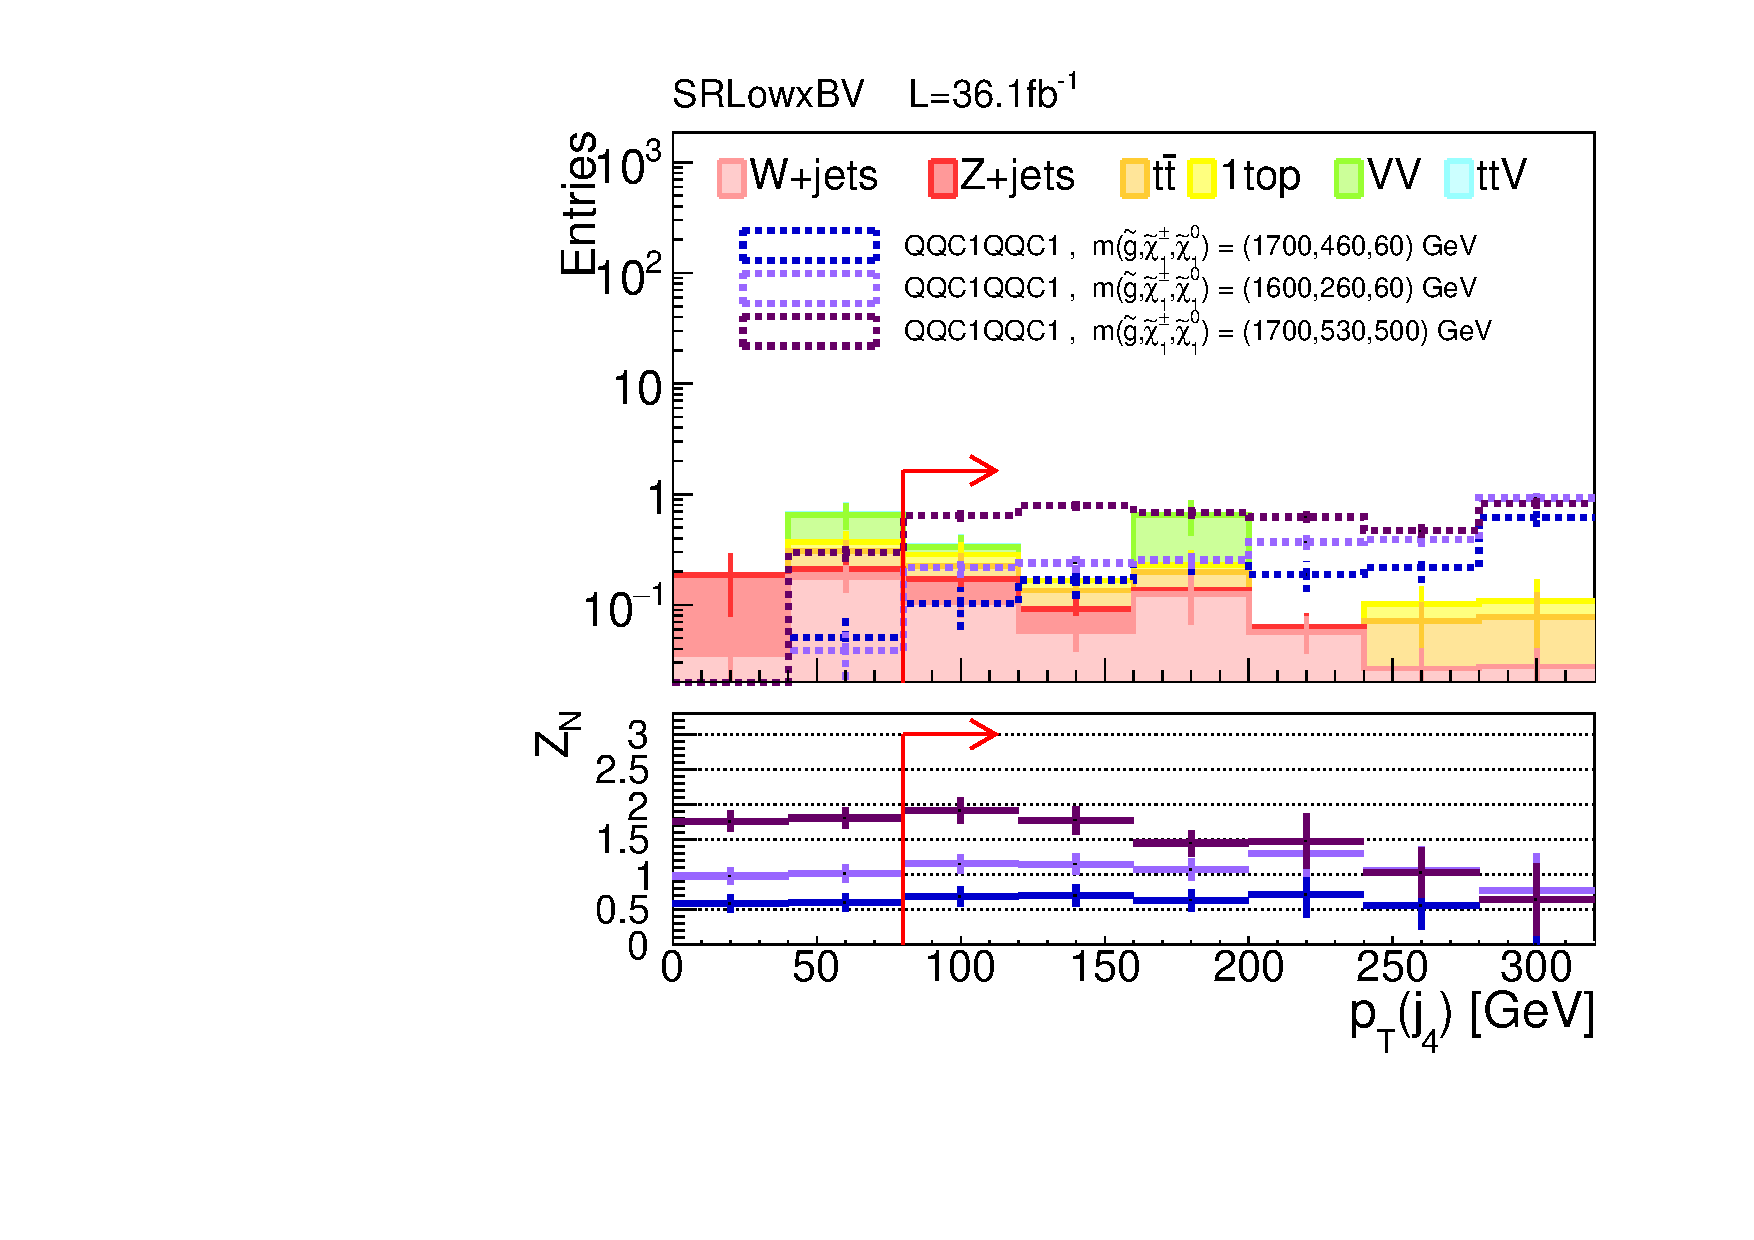
\includegraphics[width=0.45\textwidth]{figures/SRdefinition/N1plot/jet4Pt_LowxBV.pdf}}
 %   \subfigure[]{\includegraphics[width=0.45\textwidth]{figures/SRdefinition/N1plot/lep1Pt_LowxBV.pdf}}
    \subfigure[]{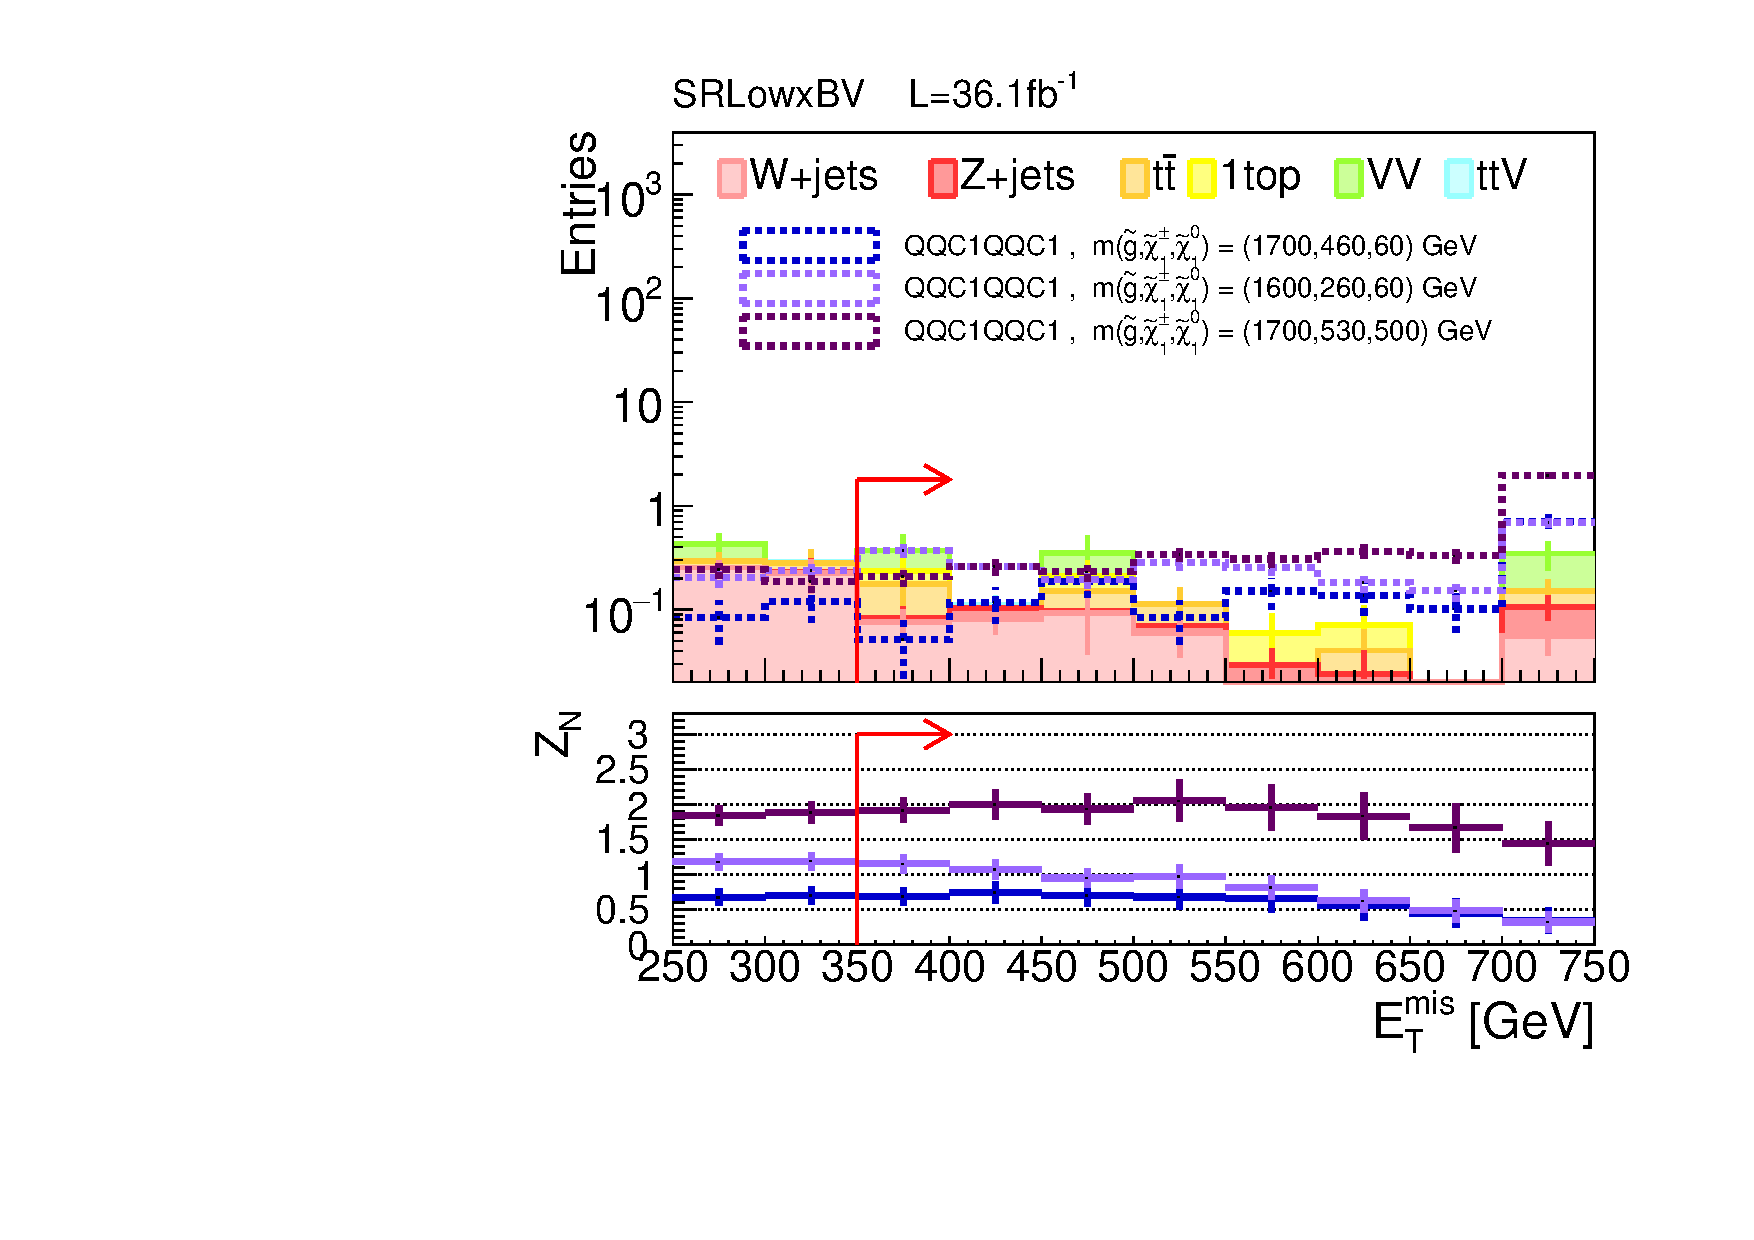
\includegraphics[width=0.45\textwidth]{figures/SRdefinition/N1plot/met_LowxBV.pdf}}
    \subfigure[]{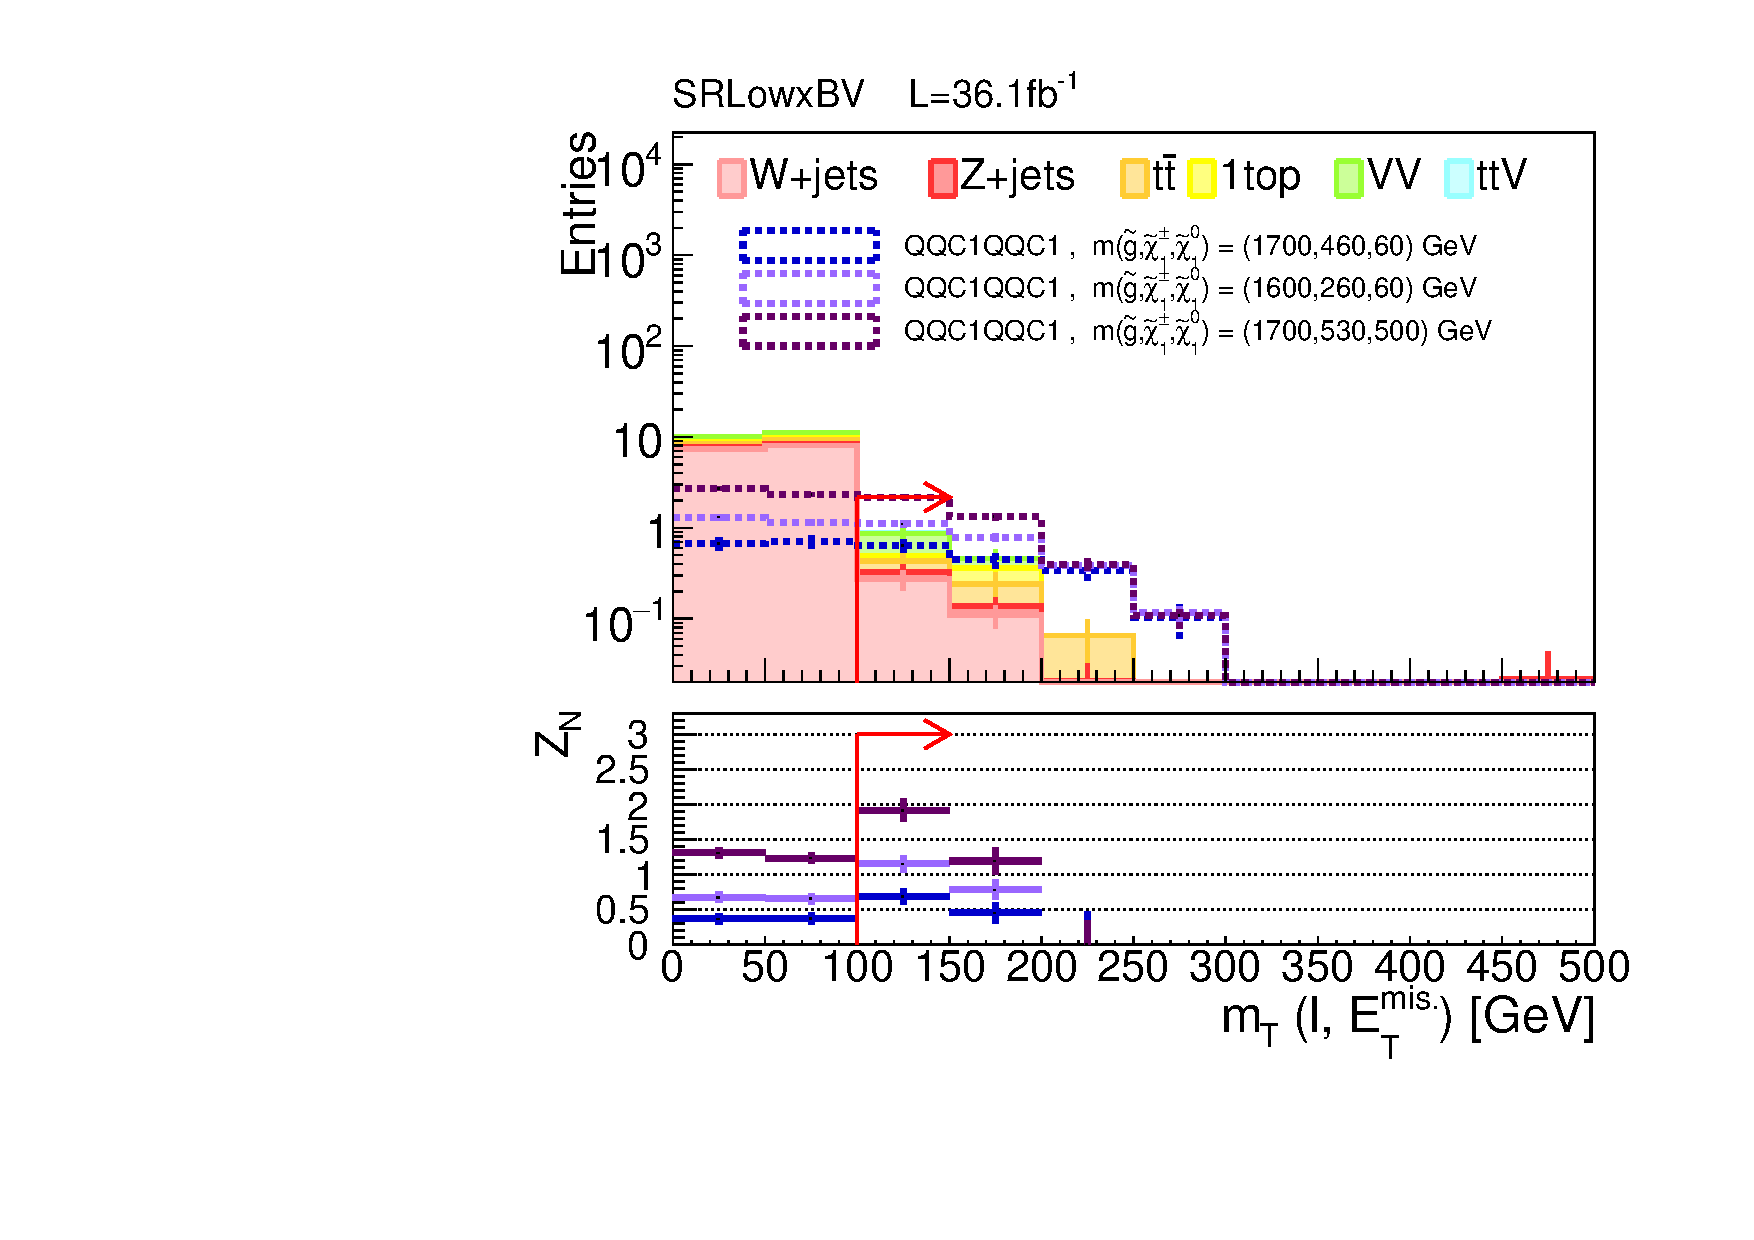
\includegraphics[width=0.45\textwidth]{figures/SRdefinition/N1plot/mt_LowxBV.pdf}}
    \subfigure[]{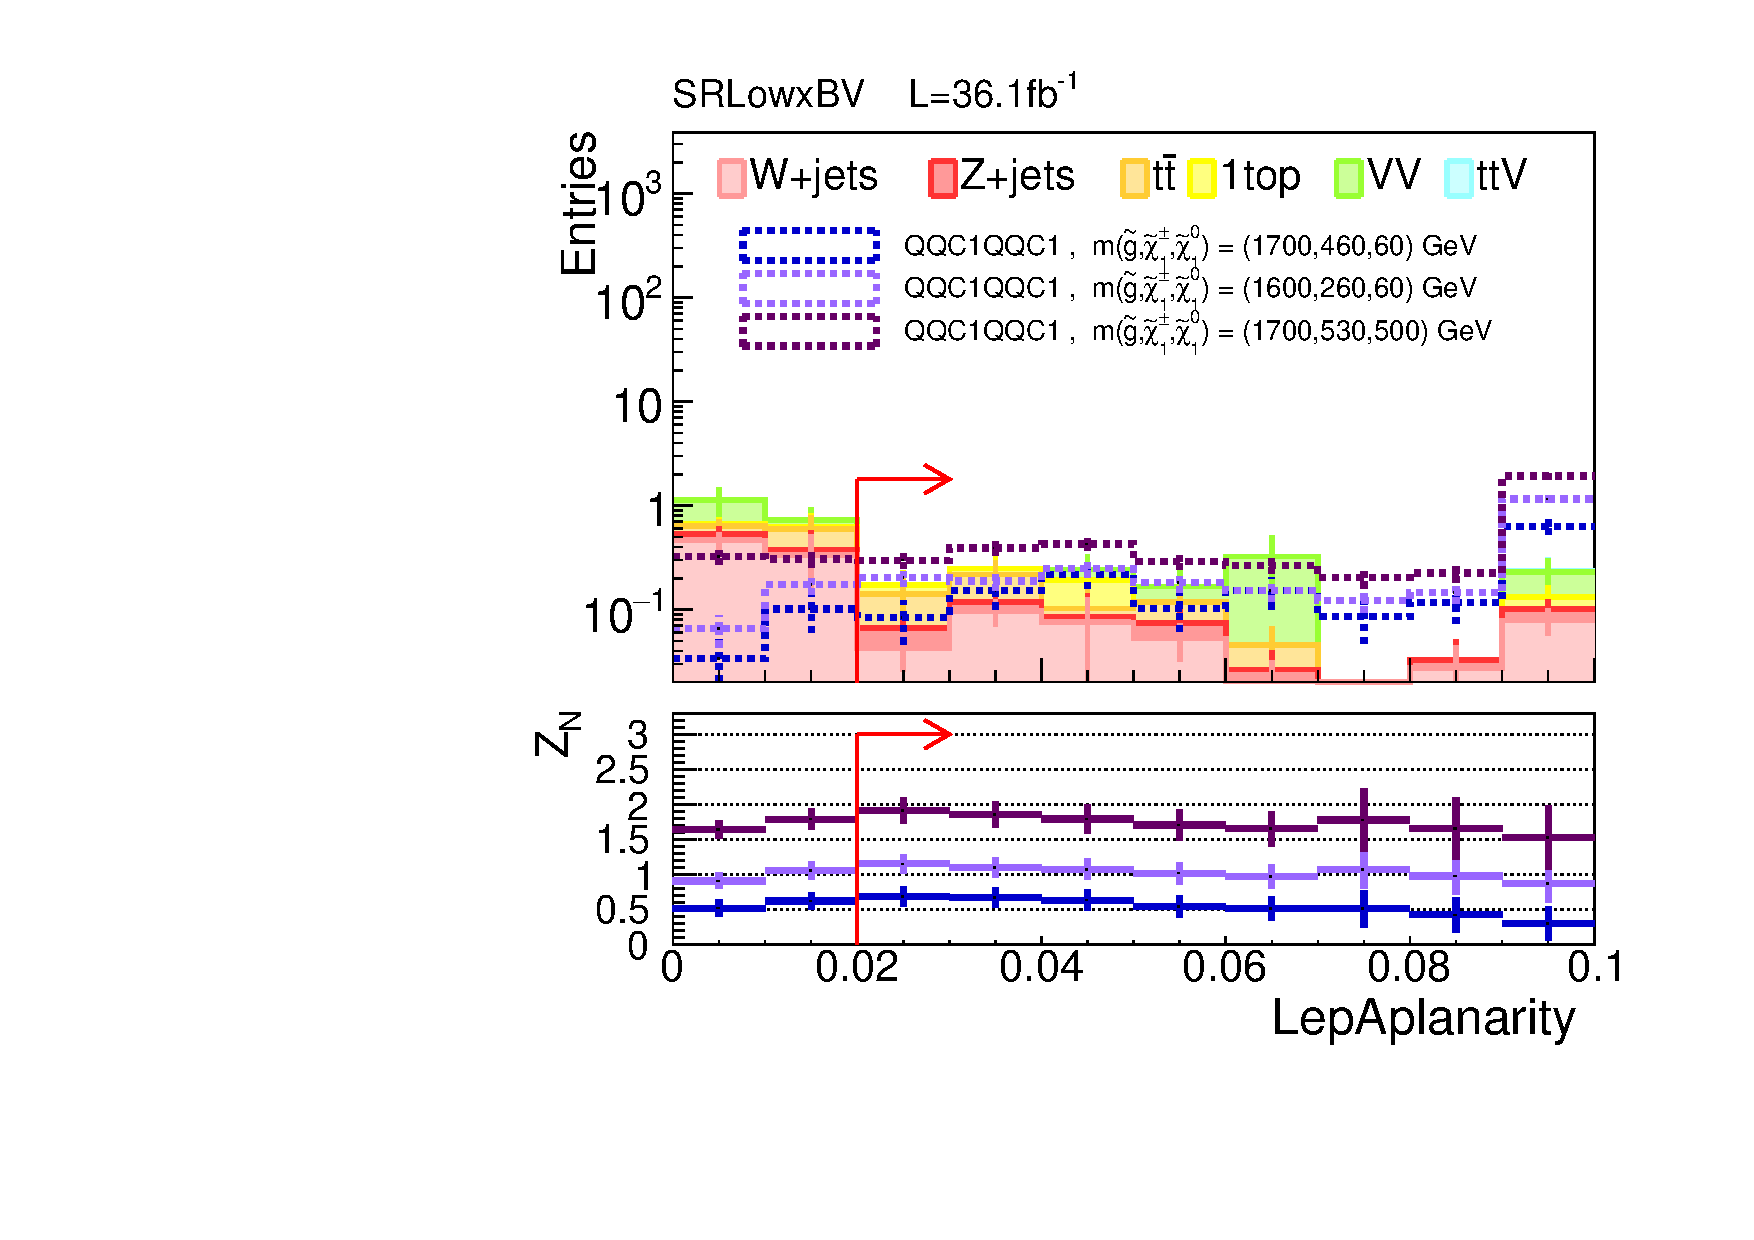
\includegraphics[width=0.45\textwidth]{figures/SRdefinition/N1plot/LepAplanarity_LowxBV.pdf}}
    \subfigure[]{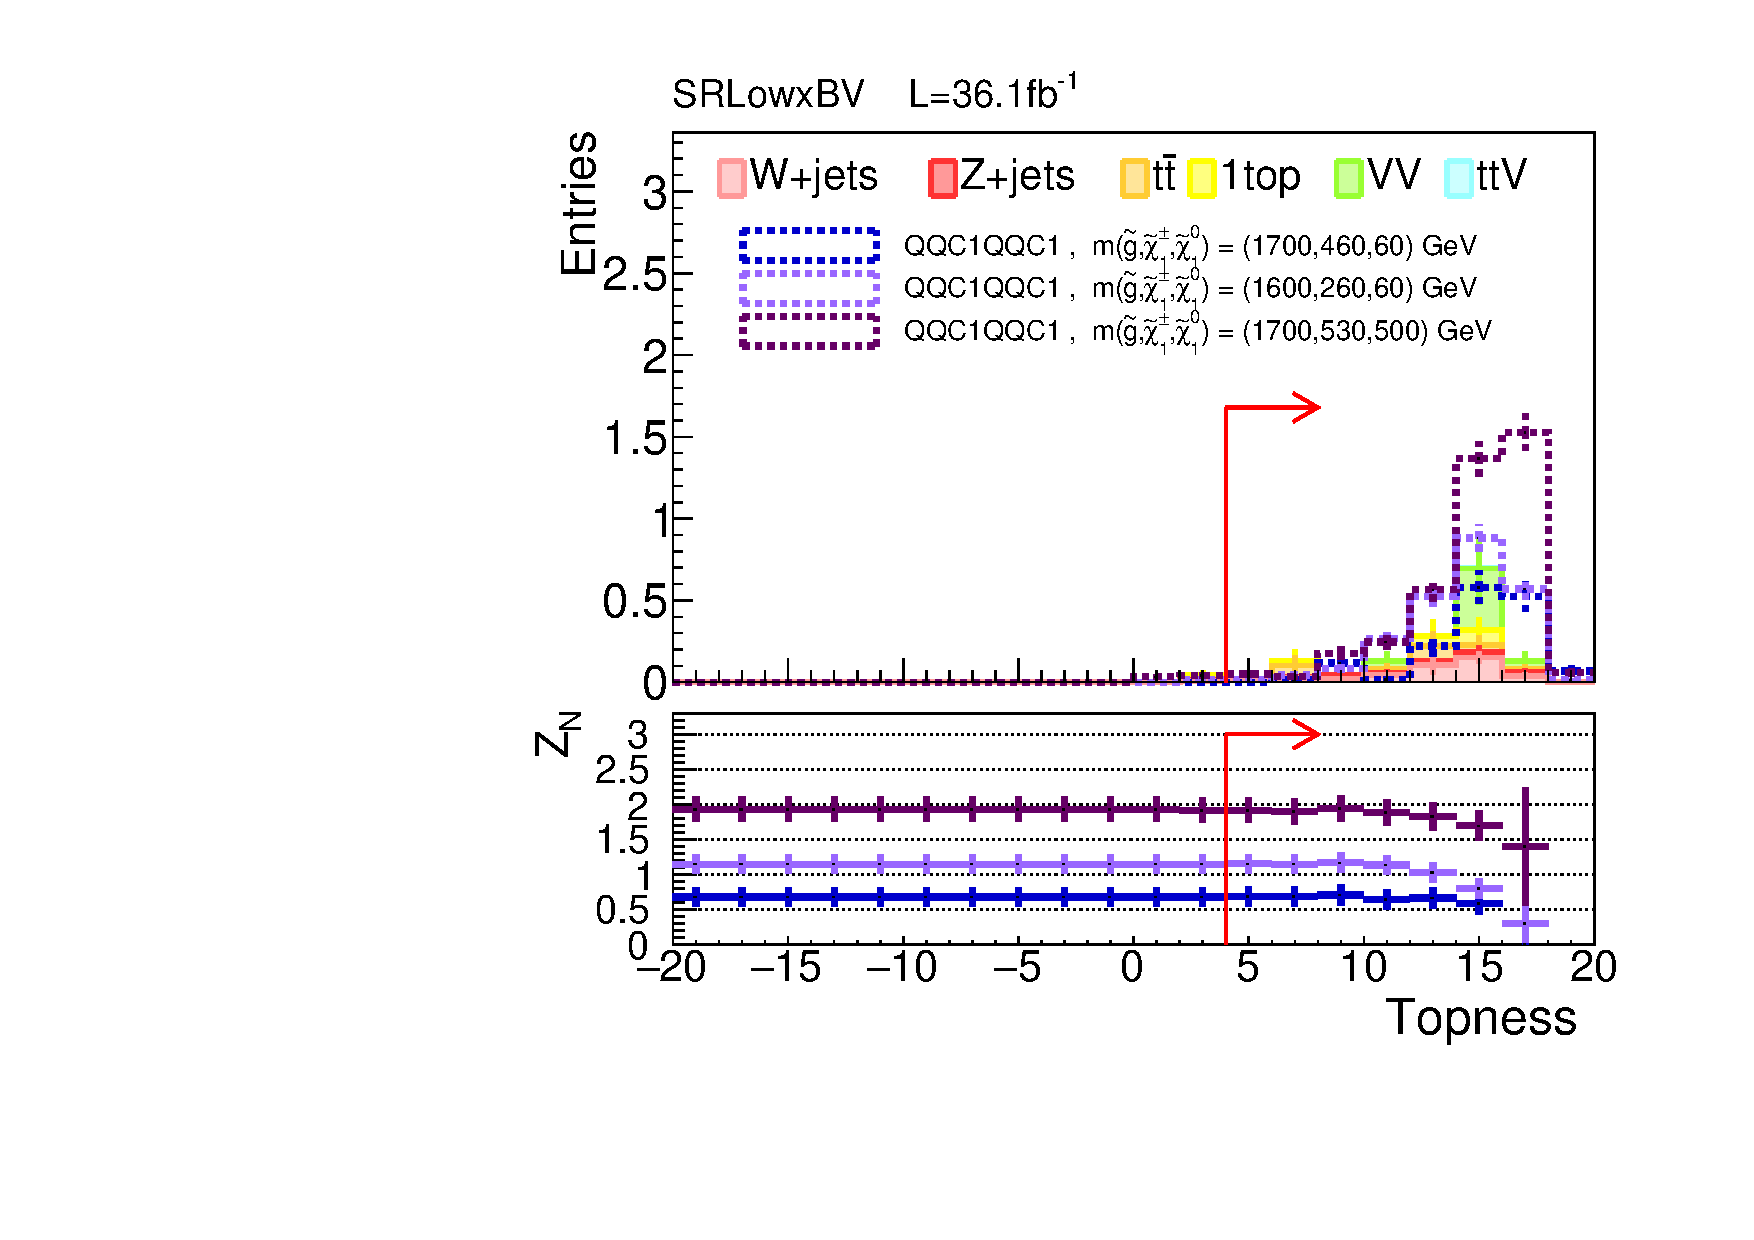
\includegraphics[width=0.45\textwidth]{figures/SRdefinition/N1plot/topNess_LowxBV.pdf}}
    \caption{ 
    N-1 plots for the b-vetoed (BV) slices of the optimized \textbf{Low-x} signal region.
    Bottom row presents the single $\meffInc$ bin significace defined in Eq. \ref{ZNcomb}. 
        \label{fig::SRdefinition::N1plots_LowxBV} 
    }
\end{figure}

\clearpage
\begin{figure}[h]
  \centering
%    \subfigure[]{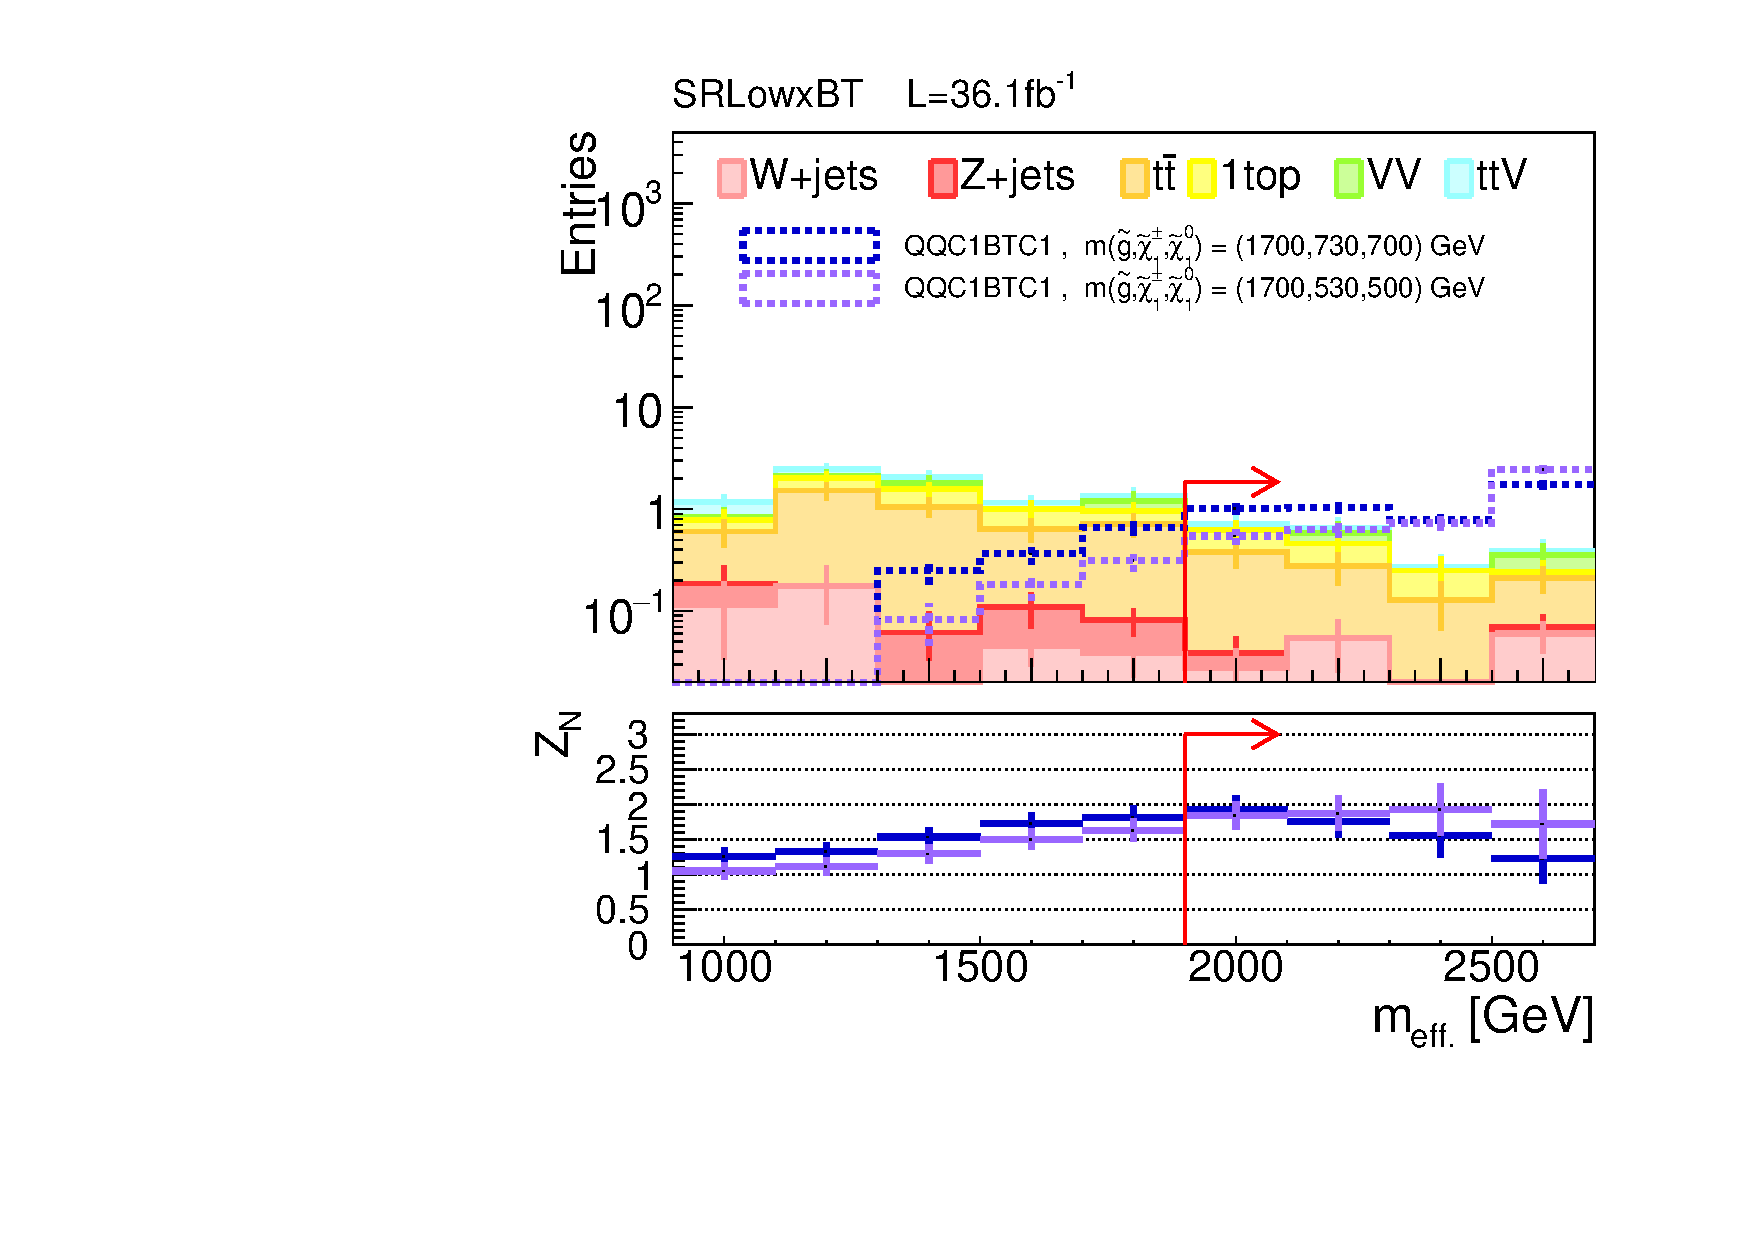
\includegraphics[width=0.45\textwidth]{figures/SRdefinition/N1plot/meffInc30_LowxBT.pdf}}
    \subfigure[]{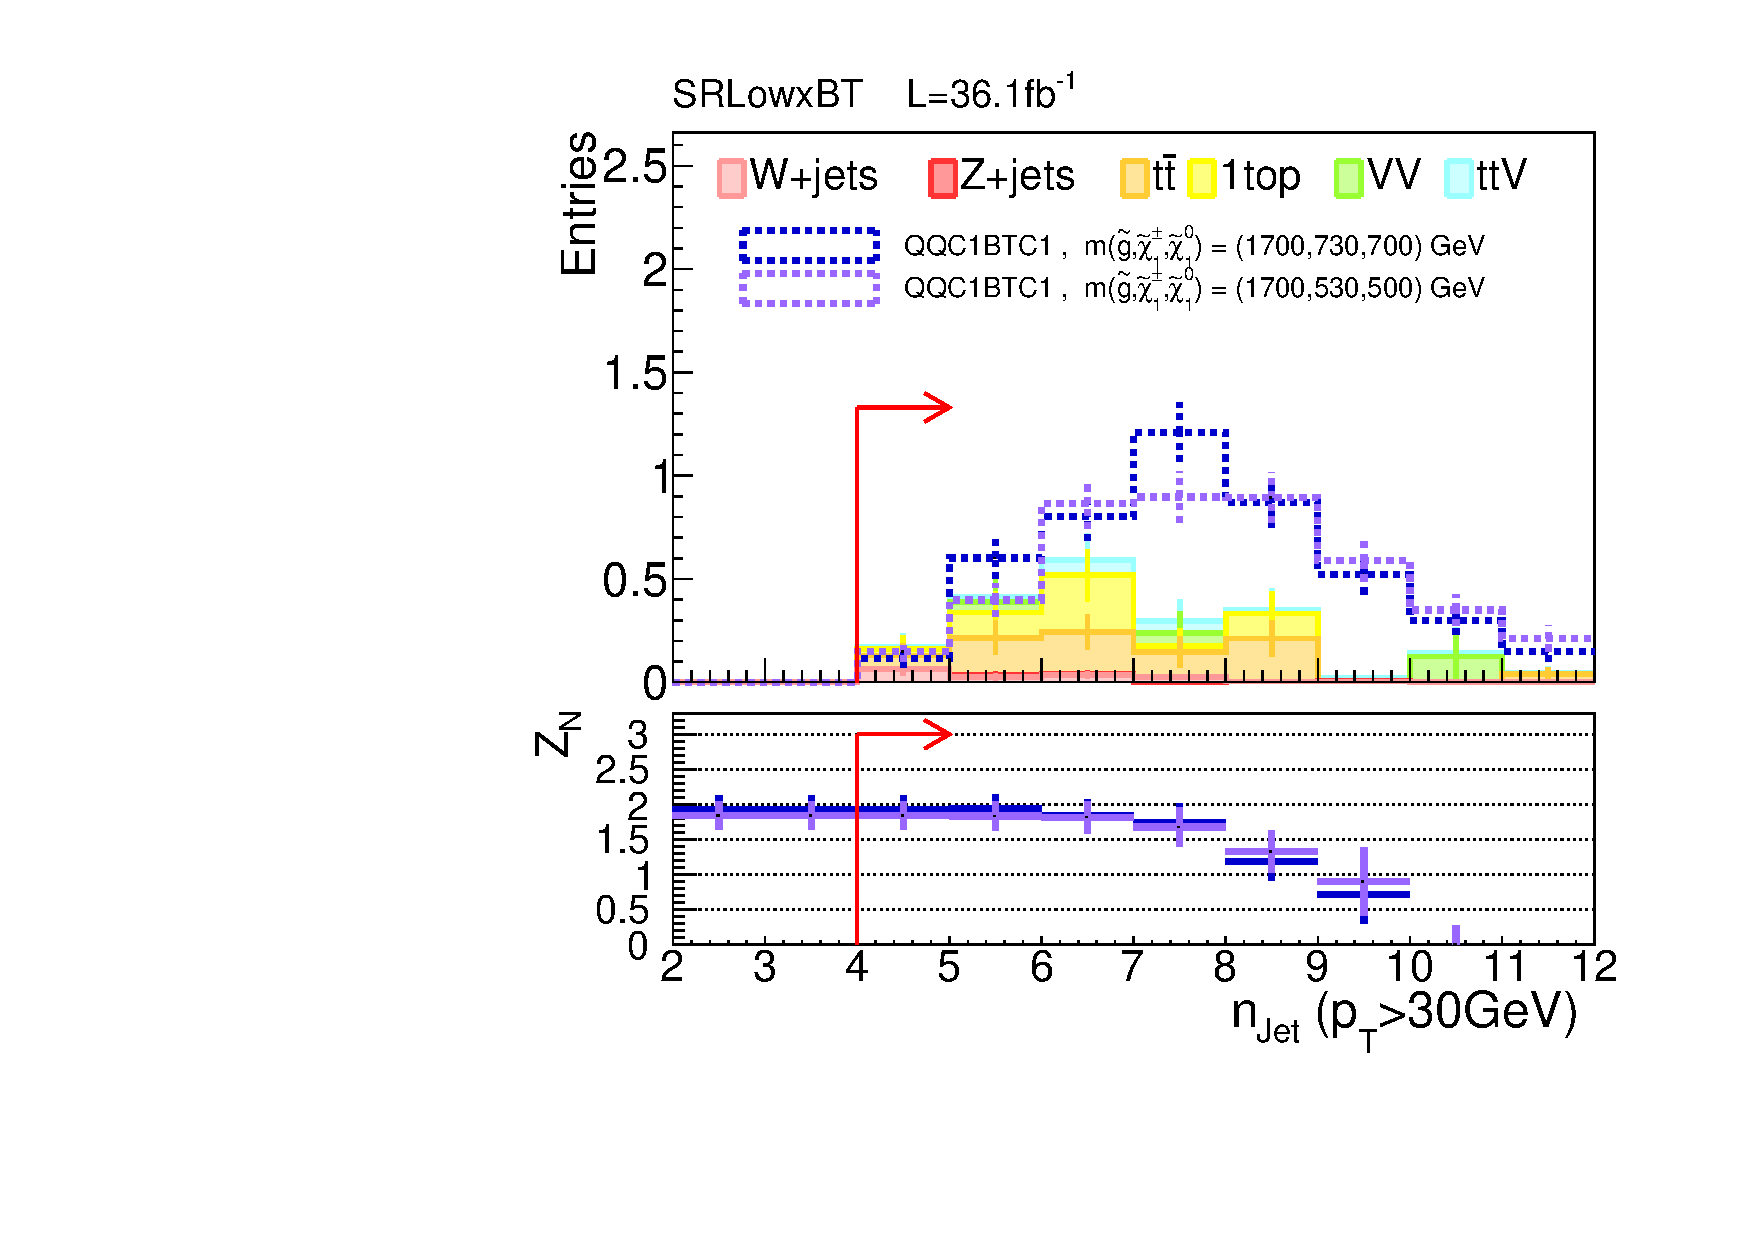
\includegraphics[width=0.45\textwidth]{figures/SRdefinition/N1plot/nJet30_LowxBT.pdf}}
    \subfigure[]{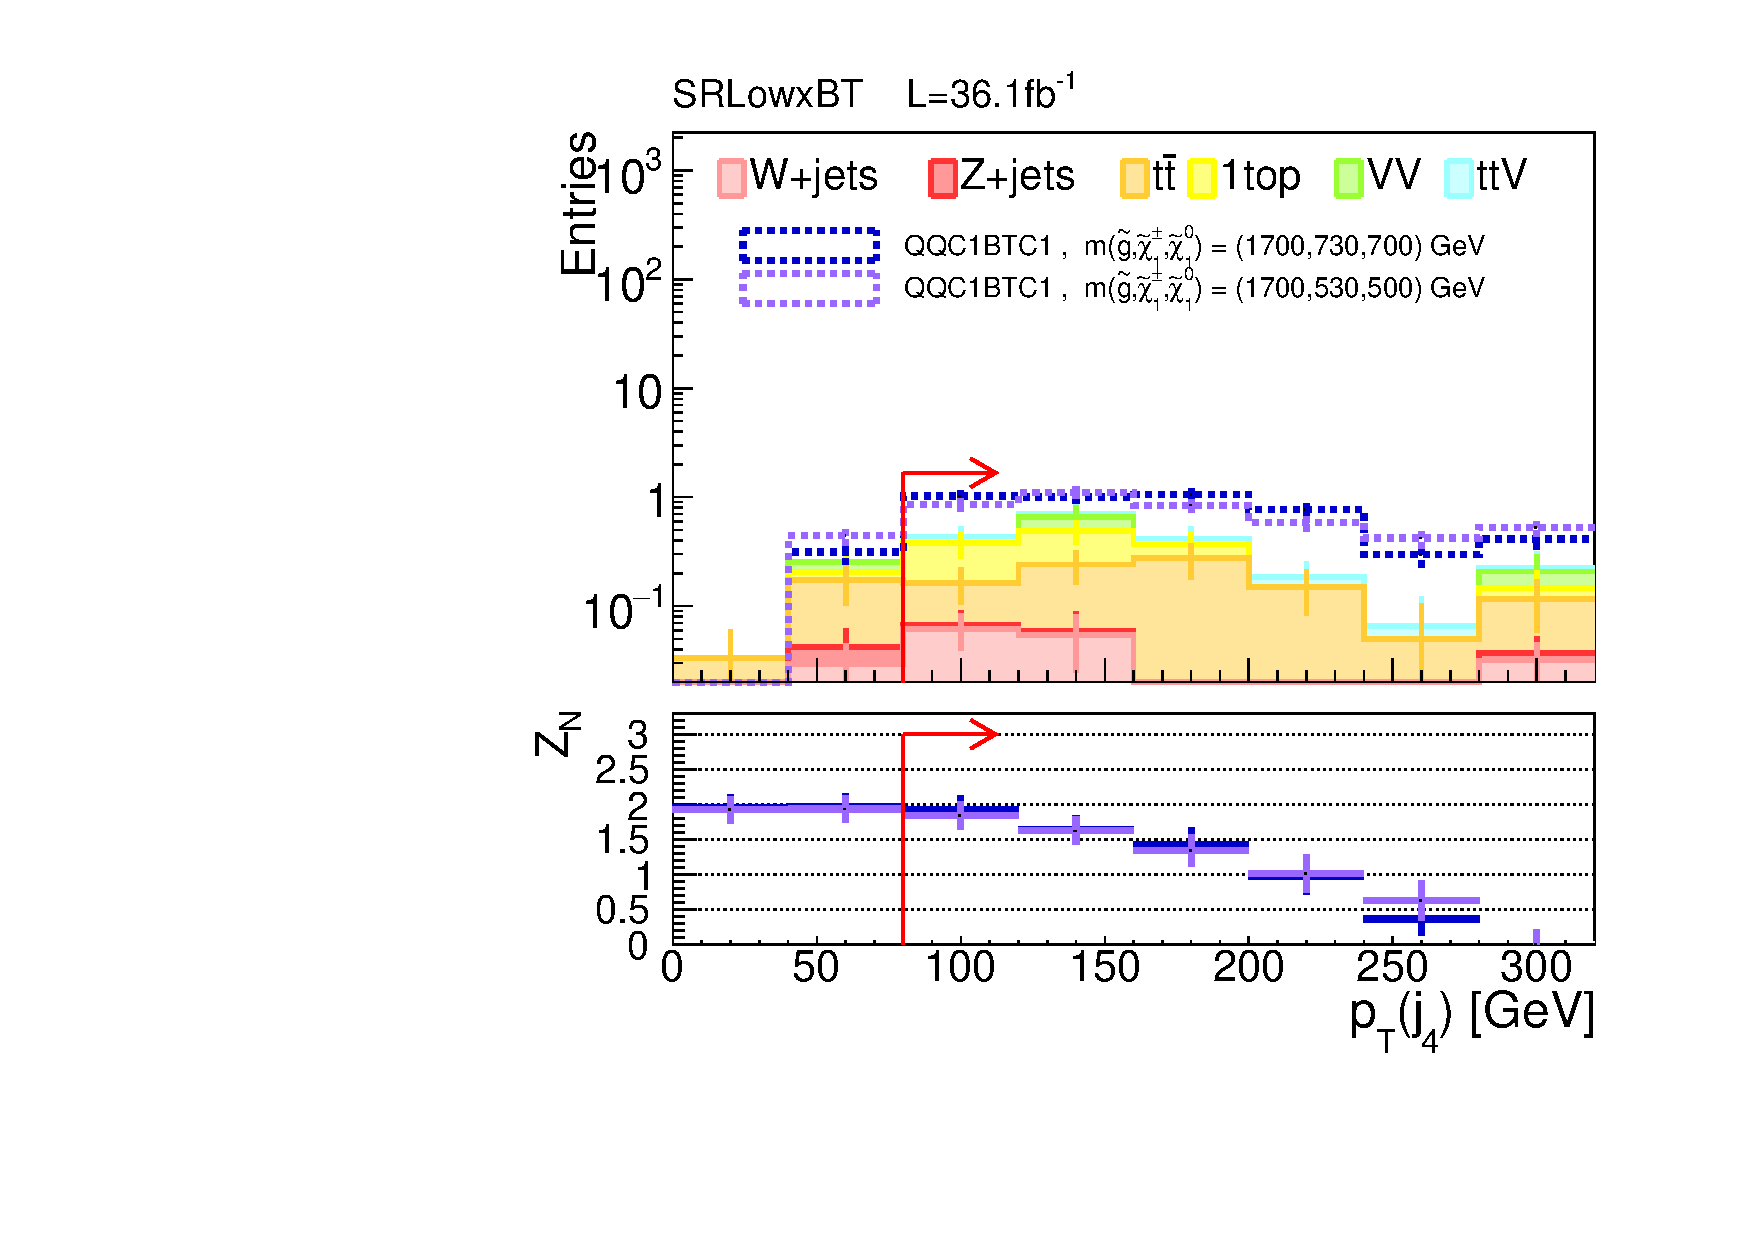
\includegraphics[width=0.45\textwidth]{figures/SRdefinition/N1plot/jet4Pt_LowxBT.pdf}}
%    \subfigure[]{\includegraphics[width=0.45\textwidth]{figures/SRdefinition/N1plot/lep1Pt_LowxBT.pdf}}
    \subfigure[]{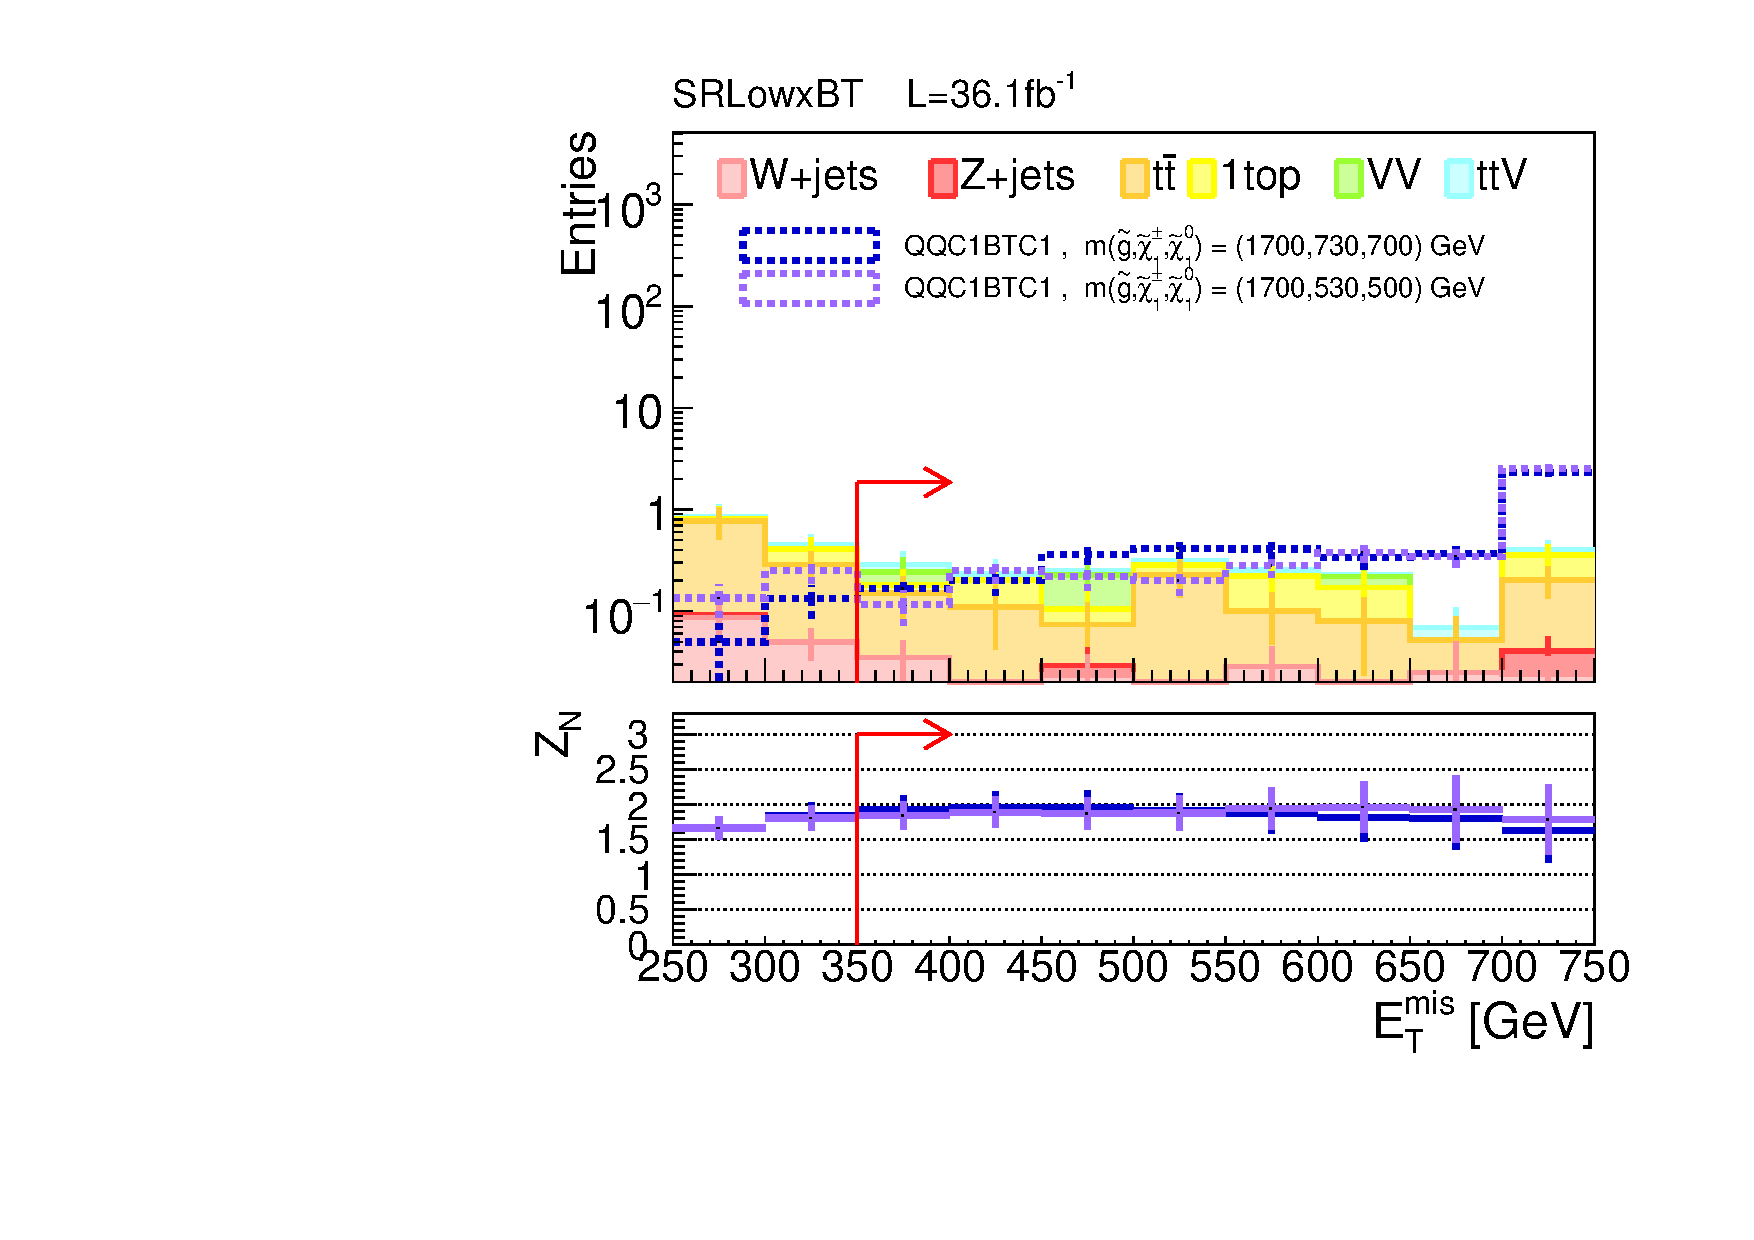
\includegraphics[width=0.45\textwidth]{figures/SRdefinition/N1plot/met_LowxBT.pdf}}
    \subfigure[]{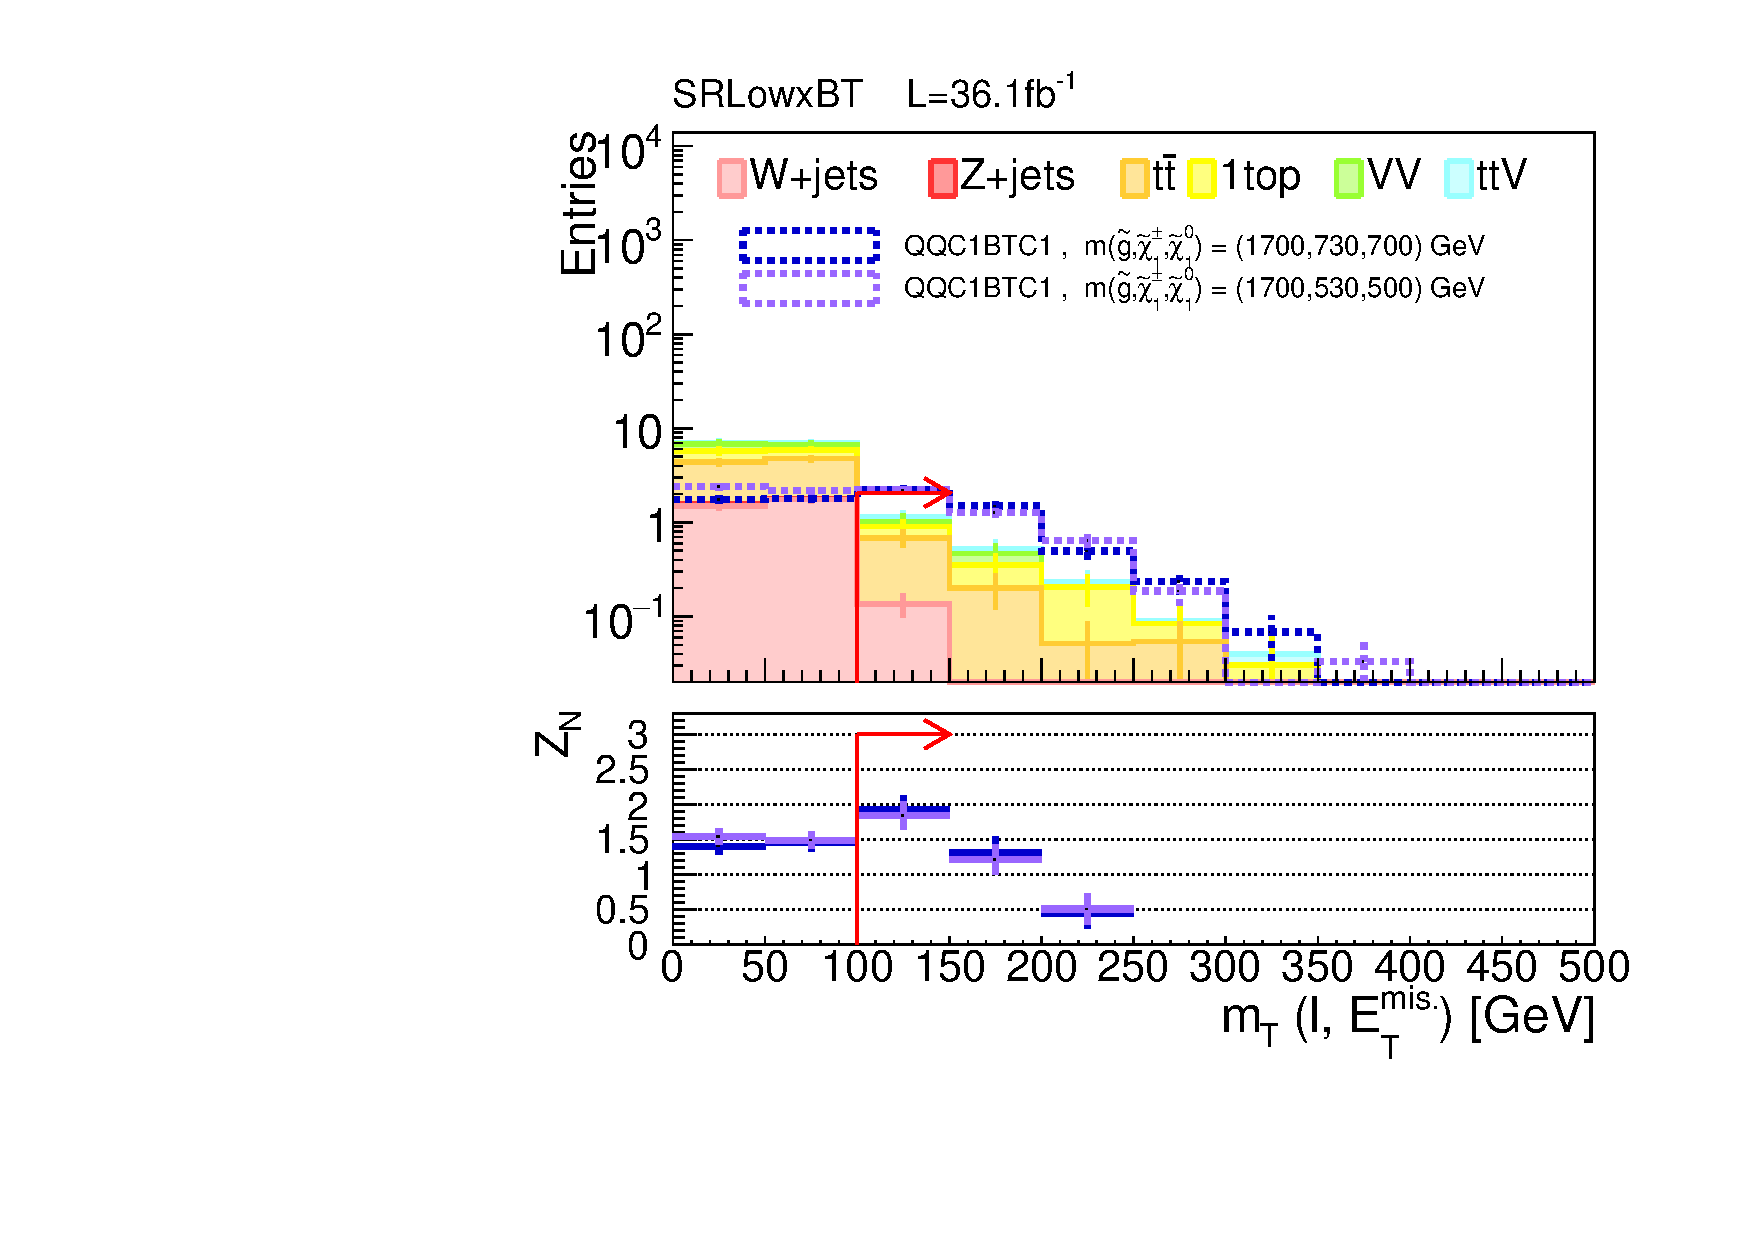
\includegraphics[width=0.45\textwidth]{figures/SRdefinition/N1plot/mt_LowxBT.pdf}}
    \subfigure[]{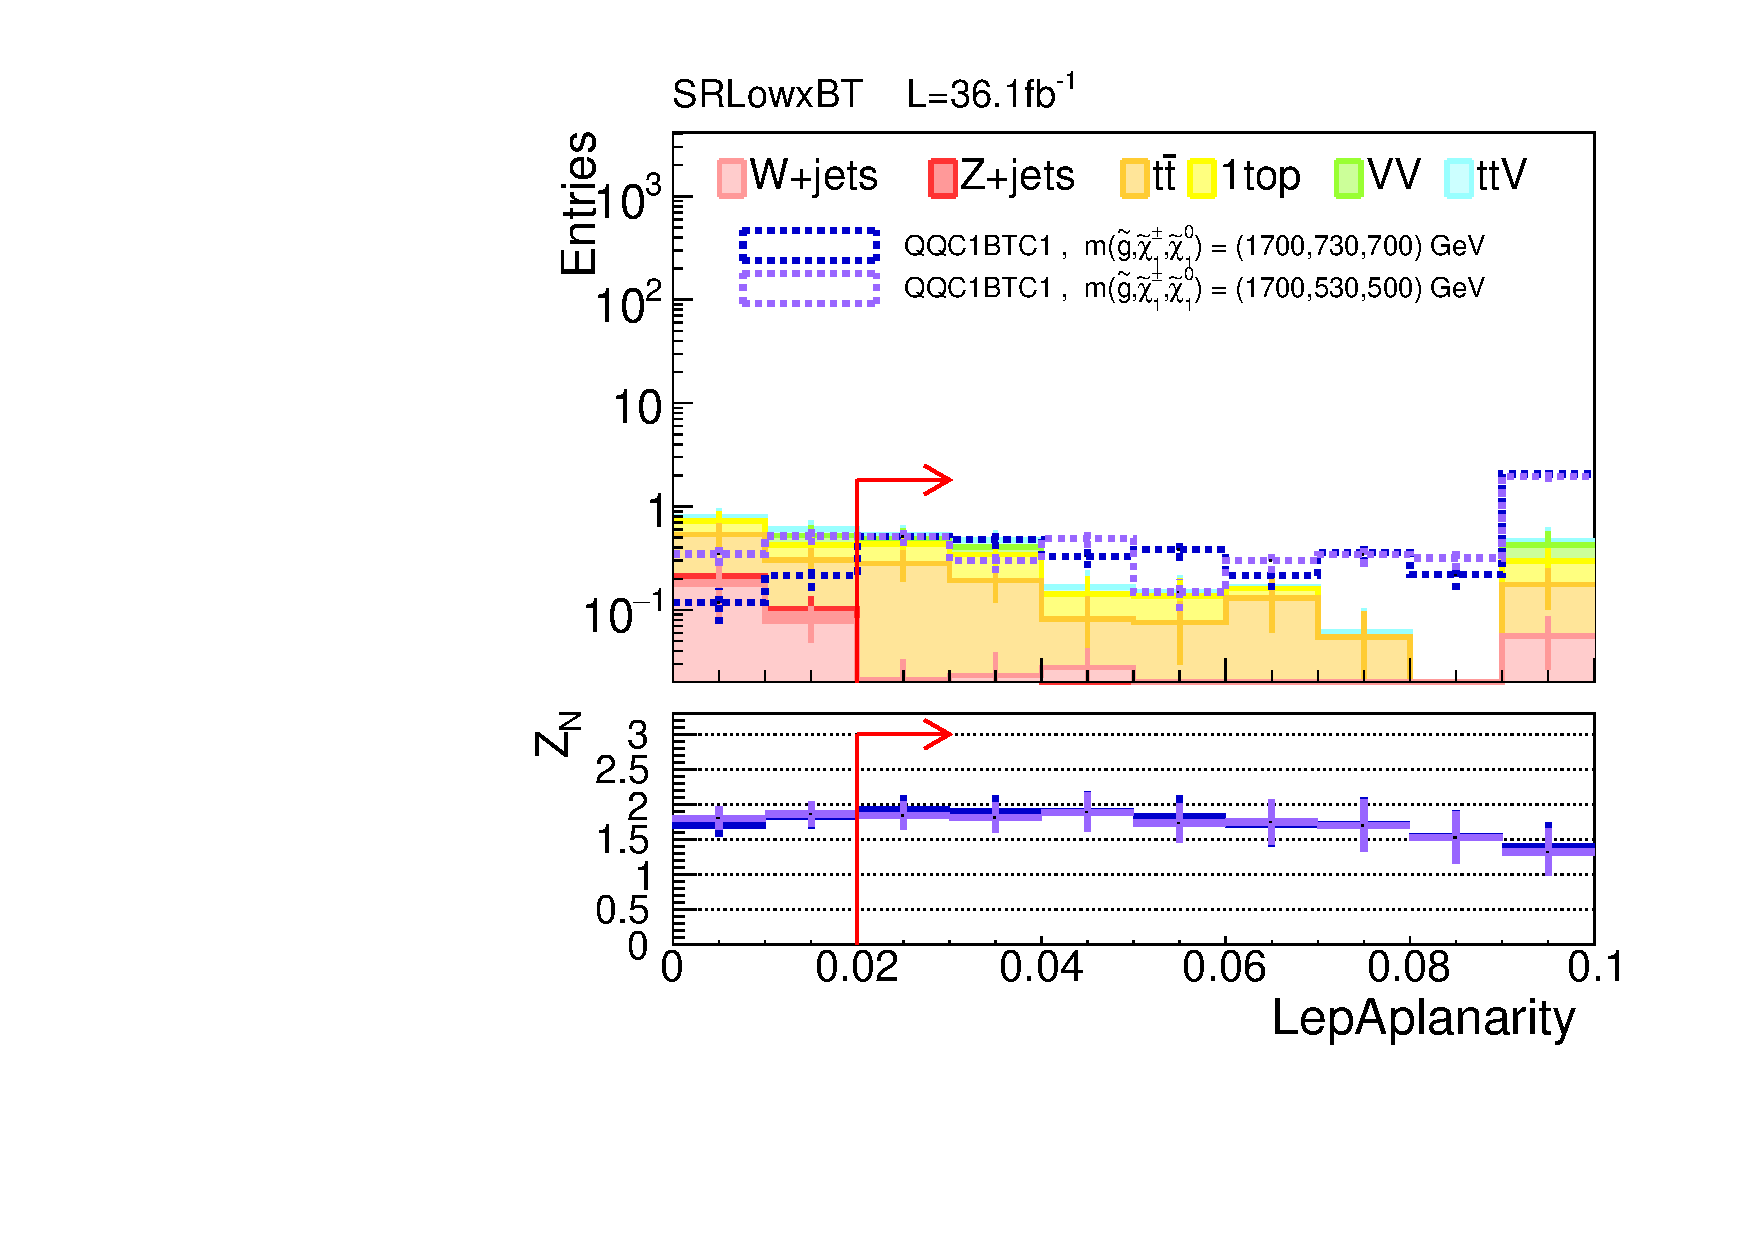
\includegraphics[width=0.45\textwidth]{figures/SRdefinition/N1plot/LepAplanarity_LowxBT.pdf}}
    \subfigure[]{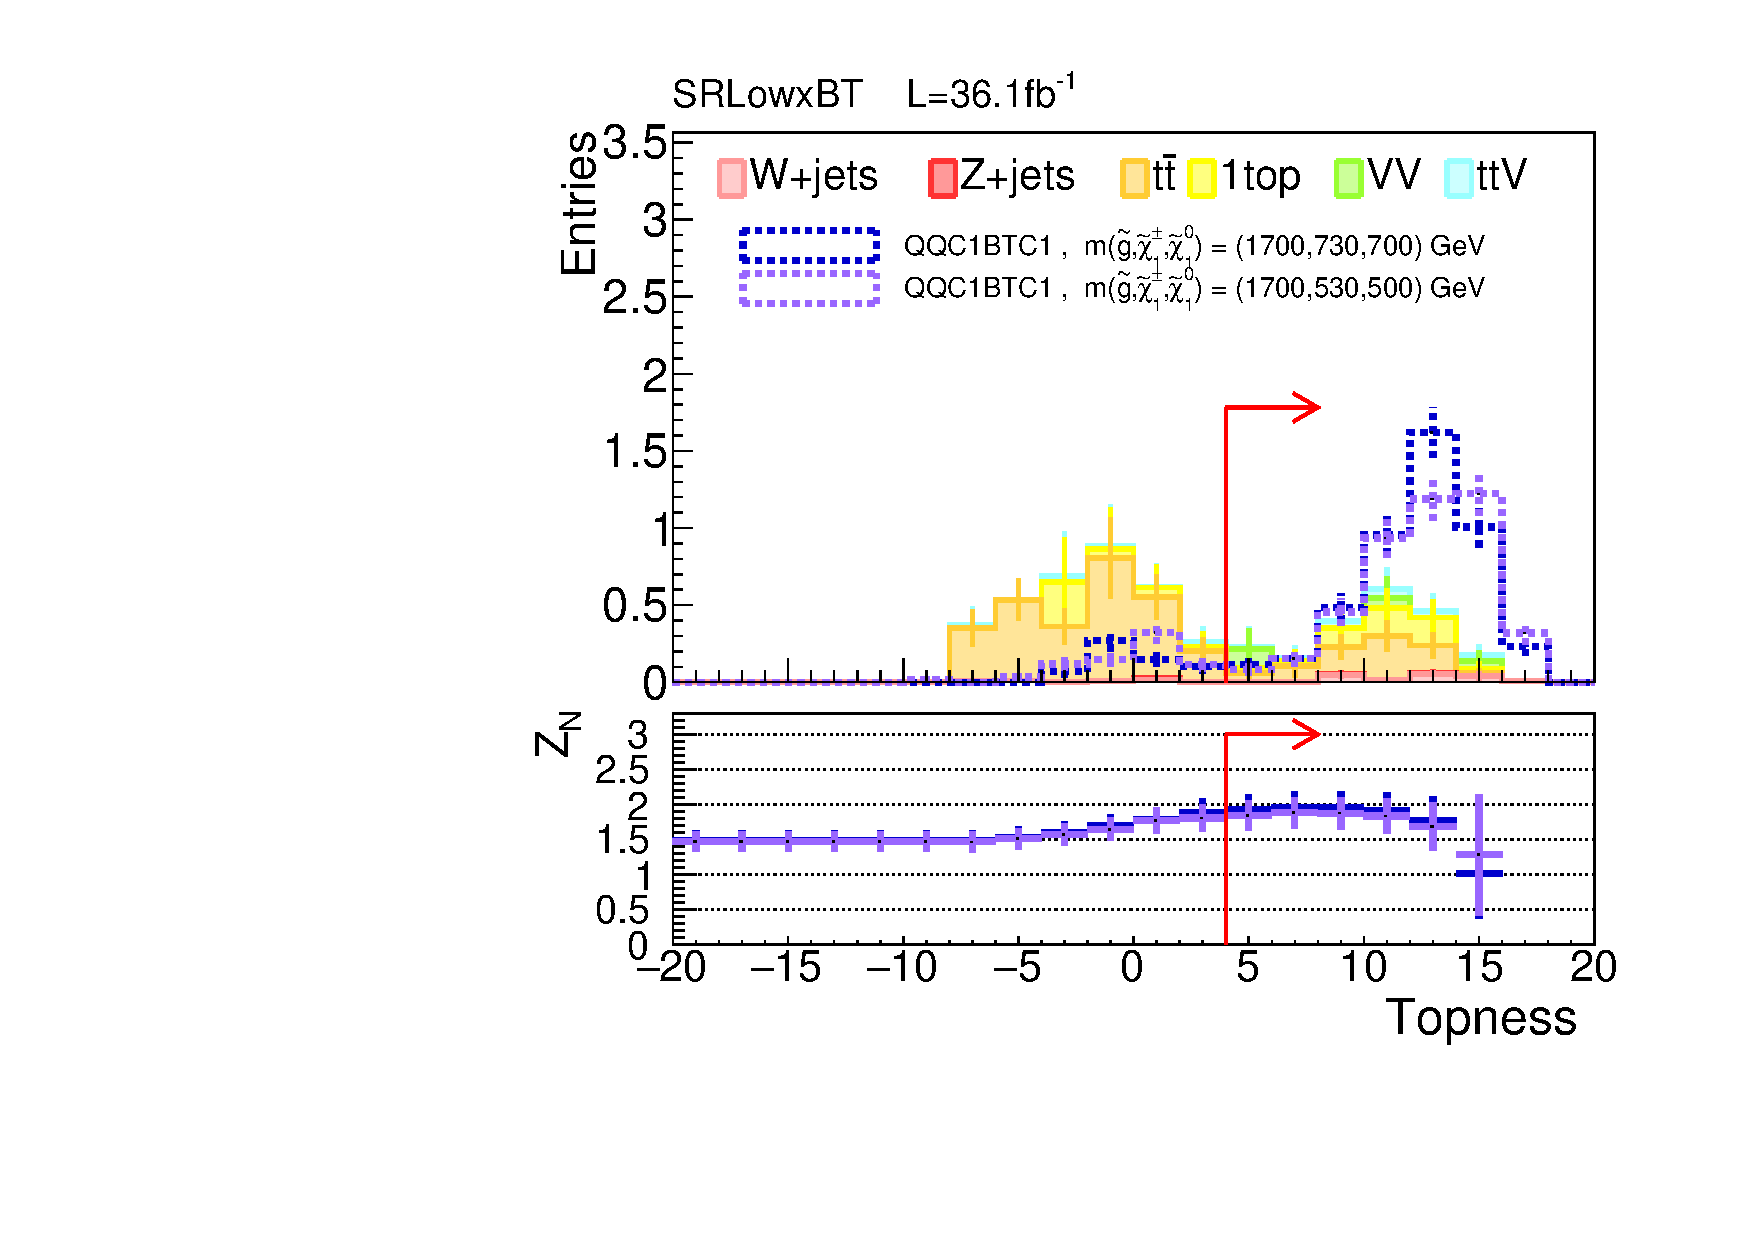
\includegraphics[width=0.45\textwidth]{figures/SRdefinition/N1plot/topNess_LowxBT.pdf}}
    \caption{ 
    N-1 plots for the b-tagged (BT) slices of the optimized \textbf{Low-x} signal region.
    Bottom row presents the single $\meffInc$ bin significace defined in Eq. \ref{ZNcomb}. 
        \label{fig::SRdefinition::N1plots_LowxBT} 
    }
\end{figure}
 

\clearpage
\begin{figure}[h]
  \centering
%    \subfigure[]{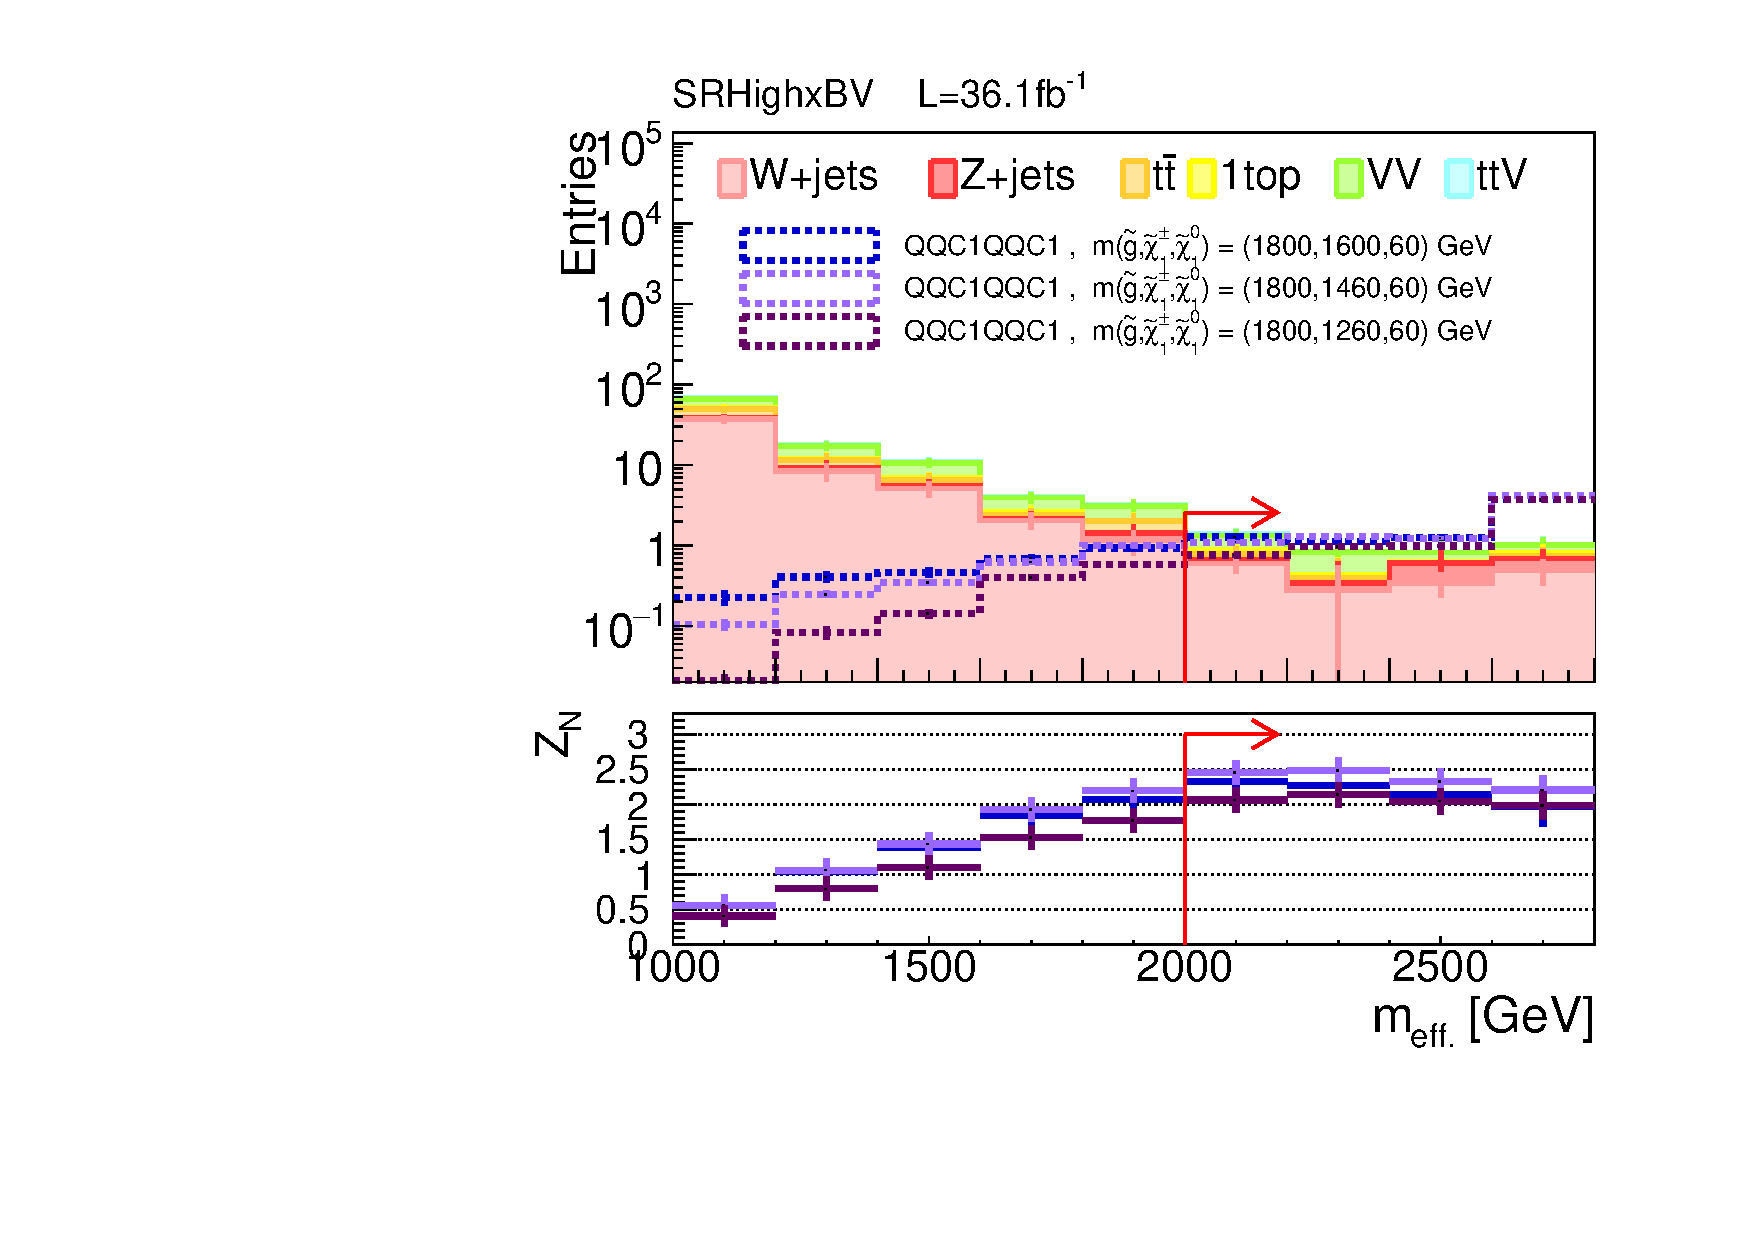
\includegraphics[width=0.45\textwidth]{figures/SRdefinition/N1plot/meffInc30_HighxBV.pdf}}
    \subfigure[]{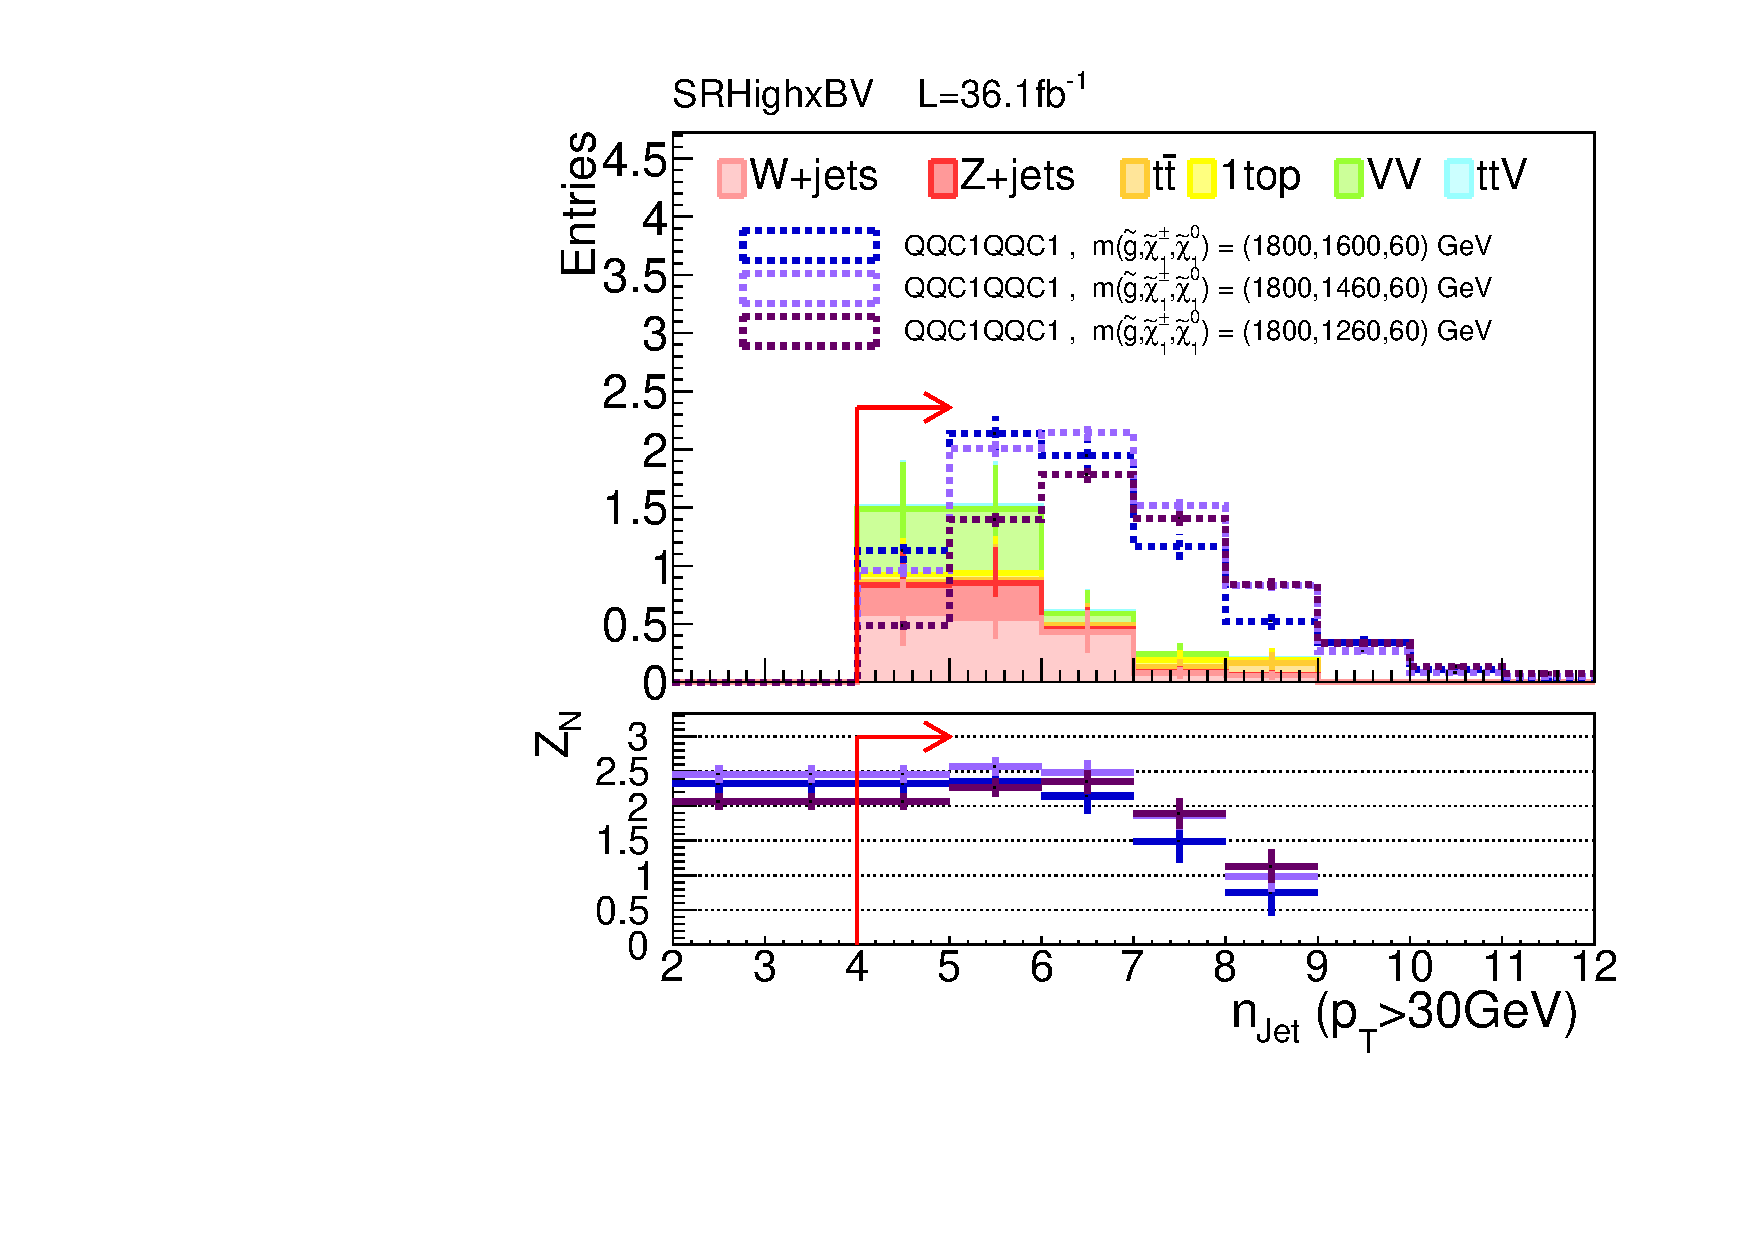
\includegraphics[width=0.45\textwidth]{figures/SRdefinition/N1plot/nJet30_HighxBV.pdf}}
%    \subfigure[]{\includegraphics[width=0.45\textwidth]{figures/SRdefinition/N1plot/lep1Pt_HighxBV.pdf}}
    \subfigure[]{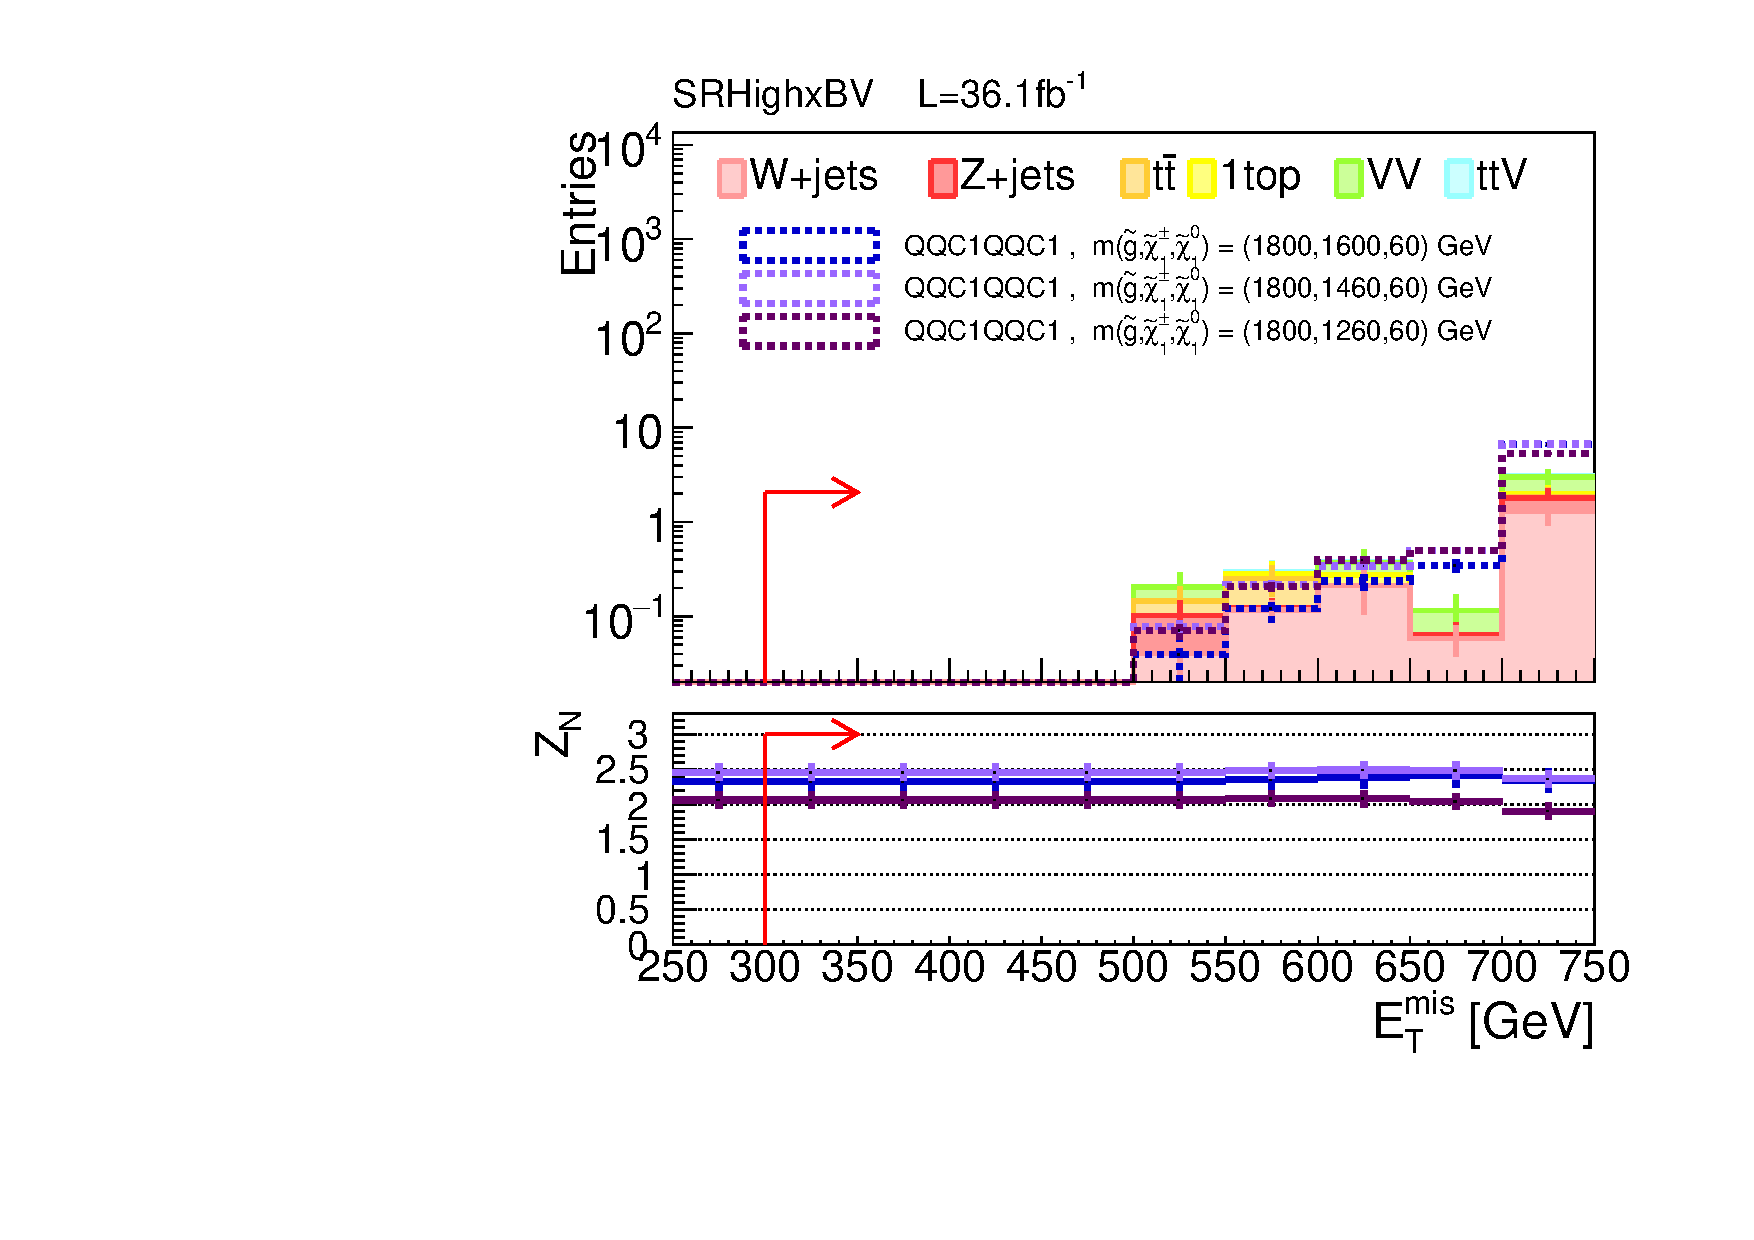
\includegraphics[width=0.45\textwidth]{figures/SRdefinition/N1plot/met_HighxBV.pdf}}
    \subfigure[]{\includegraphics[width=0.45\textwidth]{figures/SRdefinition/N1plot/mt_HighxBV.pdf}}
    \subfigure[]{\includegraphics[width=0.45\textwidth]{figures/SRdefinition/N1plot/LepAplanarity_HighxBV.pdf}}
    \subfigure[]{\includegraphics[width=0.45\textwidth]{figures/SRdefinition/N1plot/metOverMeff_HighxBV.pdf}}
    \subfigure[]{\includegraphics[width=0.45\textwidth]{figures/SRdefinition/N1plot/topNess_HighxBV.pdf}}
    \caption{ 
    N-1 plots for the b-vetoed (BV) slices of the optimized \textbf{High-x} signal region.
    Bottom row presents the single $\meffInc$ bin significace defined in Eq. \ref{ZNcomb}. 
        \label{fig::SRdefinition::N1plots_HighxBV}       
    }
\end{figure}
 

\clearpage
\begin{figure}[h]
  \centering
%    \subfigure[]{\includegraphics[width=0.45\textwidth]{figures/SRdefinition/N1plot/meffInc30_HighxBT.pdf}}
    \subfigure[]{\includegraphics[width=0.45\textwidth]{figures/SRdefinition/N1plot/nJet30_HighxBT.pdf}}
%    \subfigure[]{\includegraphics[width=0.45\textwidth]{figures/SRdefinition/N1plot/lep1Pt_HighxBT.pdf}}
    \subfigure[]{\includegraphics[width=0.45\textwidth]{figures/SRdefinition/N1plot/met_HighxBT.pdf}}
    \subfigure[]{\includegraphics[width=0.45\textwidth]{figures/SRdefinition/N1plot/mt_HighxBT.pdf}}
    \subfigure[]{\includegraphics[width=0.45\textwidth]{figures/SRdefinition/N1plot/LepAplanarity_HighxBT.pdf}}
    \subfigure[]{\includegraphics[width=0.45\textwidth]{figures/SRdefinition/N1plot/metOverMeff_HighxBT.pdf}}
    \subfigure[]{\includegraphics[width=0.45\textwidth]{figures/SRdefinition/N1plot/topNess_HighxBT.pdf}}
    \caption{ 
    N-1 plots for the b-tagged (BT) slices of the optimized \textbf{High-x} signal region.
    Bottom row presents the single $\meffInc$ bin significace defined in Eq. \ref{ZNcomb}. 
        \label{fig::SRdefinition::N1plots_HighxBT}              
    }
\end{figure}
 
\clearpage
\begin{figure}[h]
  \centering
%    \subfigure[]{\includegraphics[width=0.45\textwidth]{figures/SRdefinition/N1plot/meffInc30_3BMEFFIncl.pdf}}
    \subfigure[]{\includegraphics[width=0.45\textwidth]{figures/SRdefinition/N1plot/nJet30_3BMEFFIncl.pdf}}
%    \subfigure[]{\includegraphics[width=0.45\textwidth]{figures/SRdefinition/N1plot/lep1Pt_3BMEFFIncl.pdf}}
    \subfigure[]{\includegraphics[width=0.45\textwidth]{figures/SRdefinition/N1plot/met_3BMEFFIncl.pdf}}
    \subfigure[]{\includegraphics[width=0.45\textwidth]{figures/SRdefinition/N1plot/mt_3BMEFFIncl.pdf}}
    \subfigure[]{\includegraphics[width=0.45\textwidth]{figures/SRdefinition/N1plot/LepAplanarity_3BMEFFIncl.pdf}}
    \subfigure[]{\includegraphics[width=0.45\textwidth]{figures/SRdefinition/N1plot/min_dPhi_4j_3BMEFFIncl.pdf}}
    \subfigure[]{\includegraphics[width=0.45\textwidth]{figures/SRdefinition/N1plot/topNess_3BMEFFIncl.pdf}}
    \caption{ 
    N-1 plots for the optimized \textbf{3B} signal regions.
    Bottom row presents the combined significace over the $\meffInc$ bins defined in Eq. \ref{ZNcomb}.
        \label{fig::SRdefinition::N1plots_3BMEFFIncl}              
    }
\end{figure}
 

 
